\documentclass{book}
\usepackage[a4paper, margin=3cm]{geometry}
% \usepackage{fancyhdr}
% \pagestyle{fancy}
\usepackage[english]{babel}
\usepackage{csquotes,xpatch} % Needs to be loaded after babel
\usepackage[style=authoryear]{biblatex}
\addbibresource{bibliography.bib}

\usepackage{algorithm}
\usepackage{algpseudocode}
\usepackage{amsmath,amssymb,amsbsy,amsthm}
\usepackage{bm}
\usepackage{graphicx}
\usepackage{hyperref}
% \usepackage{mathptmx} %Times new romans text
% \usepackage{My_AMA}
\usepackage{pgfplots}
\pgfplotsset{compat=1.18}

\usepackage{setspace}
\onehalfspacing

\usepackage{subcaption}
\usepackage{tikz}
\usetikzlibrary{arrows.meta,backgrounds}
\graphicspath{ {images} }

\usepackage{todonotes}
\usepackage{xcolor}
\definecolor{ruby}{RGB}{192, 47, 29}

\newtheorem{definition}{Definition}[chapter]
\newtheorem{theorem}[definition]{Theorem}
\newtheorem{example}[definition]{Example}

\newcommand{\A}{\mathcal{A}}
\DeclareMathOperator*{\argmax}{arg\,max}
\DeclareMathOperator*{\argmin}{arg\,min}
\newcommand{\btheta}{\bm{\theta}}
\newcommand{\bx}{\mathbf{x}}
\newcommand{\by}{\mathbf{y}}
\DeclareMathOperator{\corr}{corr}
\DeclareMathOperator{\cov}{cov}
\newcommand{\D}{\mathcal{D}}
\DeclareMathOperator{\E}{\mathbb{E}}
\newcommand{\EI}{\mathrm{EI}}
\DeclareMathOperator{\Exp}{Exp}
\newcommand{\GP}{\mathcal{GP}}
\let\L\relax
\DeclareMathOperator{\L}{\mathcal{L}}
\newcommand{\LABC}{\L_\text{ABC}}
\DeclareMathOperator{\LN}{LN}
\newcommand{\LS}{\mathrm{LSE}}
\newcommand{\MLE}{\mathrm{MLE}}
\DeclareMathOperator{\MVN}{MVN}
\newcommand{\N}{\mathcal{N}}
\newcommand{\obs}{\mathrm{obs}}
% \DeclareMathOperator{\p}{\mathbb{P}}
\DeclareMathOperator{\Pois}{Pois}
\newcommand{\R}{\mathbb{R}}
\newcommand{\smtheta}{\overline{\ln\D(\btheta)}}
\newcommand{\smthetat}{\overline{\ln\D(\btheta^{(t)})}}
\DeclareMathOperator{\var}{var}

\makeatletter
\providecommand*{\diff}%
    {\@ifnextchar^{\DIfF}{\DIfF^{}}}
\def\DIfF^#1{%
    \mathop{\mathrm{\mathstrut d}}%
        \nolimits^{#1}\gobblespace}
\def\gobblespace{%
        \futurelet\diffarg\opspace}
\def\opspace{%
        \let\DiffSpace\!%
        \ifx\diffarg(%
            \let\DiffSpace\relax
        \else
            \ifx\diffarg[%
               \let\DiffSpace\relax
            \else
               \ifx\diffarg\{%
                   \let\DiffSpace\relax
               \fi\fi\fi\DiffSpace}

\begin{document}
%-----------------------front matter

\title{
{Efficient likelihood approximation via Gaussian processes: 
with an application to an existing \emph{Plasmodium vivax} malaria model}\\
{\large The University of Melbourne}
}
\author{Jacob Cumming}


\date{May 2024}

\maketitle
\pagenumbering{roman}
\tableofcontents

\listoftables
\listoffigures

% \begin{abstract}
abstrat
\end{abstract}
% \include{ack}

%\listoftodos

%\newpage
%\addcontentsline{toc}{part}{LIST OF TABLES}
%\listoftables
%\addcontentsline{toc}{part}{LIST OF FIGURES}
%\addtocontents{lot}{Table~\hfill Page \par}
%\addtocontents{toc}{CHAPTER \par}
%\addtocontents{lof}{Figure~\hfill Page \par}
%\listoffigures
\newpage
%-----------------------body
\pagenumbering{arabic}

\chapter{Introduction}

Malaria is an infectious disease that poses a significant global health 
challenge. In 2022, the World Health Organisation estimated that malaria 
caused over 600,000 
deaths, most of which were in children under five 
\parencite{world_health_organization_world_2022}. 
The majority of malaria-related deaths are attributable to the 
\textit{Plasmodium falciparum} species of the parasite. 
However, the literature is increasingly recognising that 
the amount of death and severe disease attributable to the 
\textit{Plasmodium vivax} species is 
likely traditionally underestimated. The malaria lifecycle is complicated, 
needing both a vertebrate and mosquito host. In addition, \textit{P. vivax} has 
a dormant stage that causes relapses. 

Various countries with endemic malaria have undertaken significant efforts to 
reduce the burden of or eradicate malaria. Mathematical disease models are 
increasingly aiding these efforts by helping to understand the spread of the 
disease and estimate the effectiveness of possible interventions. 
Malaria models are complex due to the many staged lifecycle, and in 
particular, \textit{P. vivax} models need to consider relapses, further 
complicating the model.

To simulate different scenarios using models, modellers must first calibrate
the model parameters to approximate observed disease dynamics, measured by
observed data such as case counts or prevalence surveys. Standard techniques
to calibrate parameters include maximum likelihood estimation and sampling
from a posterior distribution, which both require a likelihood function. As
models become increasingly complicated, analytic forms for the likelihood may
not exist, or calculating the likelihood may be very computationally
burdensome. Some researchers calibrate compartmental models by relying on
their deterministic counterparts, which is questionable, as the deterministic
model sometimes behaves differently from the stochastic model.

Modern
likelihood-free techniques, such as approximate Bayesian computation, 
have been designed to
facilitate a principled method of parameter calibration.
Various forms of approximate Bayesian computation have been widely adopted, 
however forms require 
require large numbers of model runs, which may be unfeasible or undesirable.

Drawing on concepts from approximate Bayesian computation, we aimed to improve
parameter calibration in malaria models, addressing a recognised need for
improvement. We do this by training a Gaussian process to predict how close a
model run will be to observed data. The Gaussian process approximation
can then be used to extract a synthetic likelihood which approximates the
true unknown likelihood. This allows for the use of frequentist and Bayesian
parameter inference.

The thesis follows the following outline: The literature review in Part I
discusses fundamental concepts of epidemiological modelling, covering
deterministic ordinary differential equation models, stochastic models, and
their simulation methods. It then examines malaria and reviews various malaria
models. Part I further surveys parameter inference techniques, comparing
frequentist and Bayesian approaches, and ends with discussing likelihood-free
techniques, particularly approximate Bayesian computation.
Approximate Bayesian computation then motivates using Gaussian processes to
develop a synthetic likelihood, which can be used in place of the unknown true
likelihood to use the traditional parameter calibration techniques in complex
models. Finally, Part I discusses using Bayesian acquisition functions to train
the Gaussian process efficiently.

Part II applies and extends this methodology by calibrating parameters specific
to a \textit{P. vivax} model using synthetic observed data. The results and 
discussion
section validates the method and demonstrates that the parameters that produced
the observed data are recoverable. Finally, the thesis concludes with a
discussion of the findings and outlines avenues for future research.
% \part{Literature Review}
% \chapter{Epidemiological Modelling}

In order to study the behaviour and characteristics of disease spread and
eradication, compartmental epidemiological models have been developed. They
seek to simplify the dynamics of a disease down to a mathematically
representable form. Inference on these models allow for an understanding of how
the modelled disease spreads, and allows an assessment of how effective
differing disease interventions (such as treatments or vaccinations) may be
without the need for large long term trials. Models can also simulate various
scenarios such as increases or decreases in viral transmission.

Simple compartmental disease models assume individuals can be only be in one of
a finite number of states (which are called compartments). These compartments
usually correspond to a state of disease. Some simple common compartments
include: \begin{itemize}
    \item $S$ - Susceptable: at risk of contracting the disease
    \item $E$ - Exposed: contracted the disease but not yet transmitting it
    \item $I$ - Infectious (also called Infected): at risk of transmitting the
          disease
    \item $R$ - Recovered: neither at risk of contracting or transmitting the
          disease.
\end{itemize}

\begin{figure}[htbp]
    \centering
    \begin{subfigure}[b]{0.18\textwidth}
        \begin{tikzpicture}[thick]
            \node[draw, minimum size=0.8cm] (S) {$S$};
            \node[draw, right=of S, minimum size=0.8cm] (I) {$I$};
            \draw[->] (S) edge[in = 160, out = 20] node
            [midway, label=above:{$\lambda_t$}] (lambda) {} (I);
            \draw[->] (I) edge[in = 340, out = 200] node
            [midway, label=below:{$\gamma$}] (gamma) {} (S);
            \draw[->, dashed, ruby] (I) edge[in = 45, out = 90] (lambda);
            % \draw (current bounding box.south east) rectangle
            % (current bounding box.north west);
        \end{tikzpicture}
        \caption{$SIS$ model}\label{fig:SIS_model}
    \end{subfigure}%
    \hfill%
    \begin{subfigure}[b]{0.18\textwidth}
        \begin{tikzpicture}[thick]
            \node[draw, minimum size=0.8cm] (S) {$S$};
            \node[draw, right=of S, minimum size=0.8cm] (I) {$I$};
            \draw[->] (S) edge node [midway, label=above:{$\lambda_t$}]
            (lambda) {} (I);
            \draw[->, dashed, ruby] (I) edge[in = 270, out = 225] (lambda);
            \node[above=of S] (mu) {};
            \node[below=of S] (S_nu) {};
            \node[below=of I] (I_nu) {};
            \draw[->] (mu) edge node [midway, label=left:{$\mu$}] () {} (S);
            \draw[->] (S) edge node [midway, label=left:{$\nu$}] () {} (S_nu);
            \draw[->] (I) edge node [midway, label=left:{$\nu + \gamma$}] () {}
            (I_nu);
            % \draw (current bounding box.south east) rectangle
            % (current bounding box.north west);
        \end{tikzpicture}
        \caption{$SI$ with demography model}\label{fig:SI_demog_model}
    \end{subfigure}%
    \hfill%
    \begin{subfigure}[b]{0.45\textwidth}
        \begin{tikzpicture}[thick]
            \node[draw, minimum size=0.8cm] (S) {$S$};
            \node[draw, minimum size=0.8cm, right=of S] (E) {$E$};
            \node[draw, minimum size=0.8cm, right=of E] (I) {$I$};
            \node[draw, minimum size=0.8cm, right=of I] (R) {$R$};
            \draw[->] (S) edge node [midway, label=above:{$\lambda_t$}]
            (lambda) {} (E);
            \draw[->] (E) edge node [midway, label=above:{$\sigma$}]
            (sigma) {} (I);
            \draw[->] (I) edge node [midway, label=above:{$\gamma$}]
            (r) {} (R);
            \draw[->, dashed, ruby] (I) edge[in = 270, out = 270] (lambda);
            % \draw (current bounding box.south east) rectangle
            % (current bounding box.north west);
        \end{tikzpicture}
        \caption{$SEIR$ model}\label{fig:SEIR_model}
    \end{subfigure}%
    \caption{
        Some simple model schematics, with varying numbers of compartments: $S$
        (susceptable), $E$ (exposed), $I$ (infectious) and $R$ (recovered). The
        force of infection $\lambda_t$ is usually a function of $I_t$, depicted
        by the dashed red lines. $\mu$ and $\nu$ are natural birth and death
        rates respectively. $\gamma$ is the rate of progression out of the
        infectious state. In each of these models the physical interpretation
        differs slightly. In the $SIS$ and $SEIR$ models, it is the rate at
        which individuals move from infectious to susceptable again or into
        lifelong immunity, whereas in the $SI$ with demography model, it can be
        interpreted as the increase to the rate of death attributable to
        disease induced mortality. $\sigma$ is the rate of progression from a
        state of latent infection to becoming infectious.
    }\label{fig:simple_models}
\end{figure}

The number of people in each compartment at time $t$ is a (possibly
non-deterministic) function of time $t,$ which we indicate as a subscript $t$
(eg.\ $S_t$ is the number of susceptibles at time $t$). Models are routinely
described by the compartments they contain. For example, an $SIS$ model, is a
model with the susceptable and infectious compartments. Recovering from the
infection leaves you susceptible to reinfection (for example most sexually
transmitted diseases \parencite[56]{keeling_modeling_2008}), and is graphically
depicted in Figure \ref{fig:SIS_model}.

Furthermore we can also include demography into a compartmental model. Diseases
that infect the individual until the time of death such as bovine spongiform
encephalopathy (BSE commonly known as mad cow disease) may be modelled using an
$SI$ model with demography (birth and death rates), as depicted in Figure
\ref{fig:SI_demog_model} \parencite{hagenaars_epidemiological_2006}.

Childhood diseases such as varicella (chickenpox) which give lifetime immunity
after infection can be modelled using an $SEIR$ model (see Figure
\ref{fig:SEIR_model}), particularly when modelling a local outbreak setting
(for example \cite{zha_research_2020} used the $SEIR$ model to model a school
outbreak of varicella). Not including demograpy is usually appropriate when
disease induced mortality is low.

The number (and names) of compartments can be extended and configured as
needed, and compartments could be added for vaccinated individuals, quarantined
individuals and so on. By convention $N_t$ (often simply $N$ in models with a
closed population) is the total number of individuals in the model, the sum of
all compartments.

\section{Deterministic ODE models}

Diseases are often simulated as deterministic ordinary differential equations.
For the examples below we assume that the force of infection $\lambda_t$ is
proportional to the number of people in $I$, such that
$\lambda_t := \beta \frac{I_t}{N_t}.$ $\beta$ can be interpreted as the average
number of people that an individual interacts with per day in a way such that
disease would be spread in that interaction per unit of time $t$. This is
sometimes called the effective contact rate. Therefore since $\frac{I_t}{N_t}$
is the probability that a randomly selected individual is infectious,
$\beta \frac{I_t}{N_t}$ can be interpreted as the average number of people that
a person interacts with each day who are infectious in a way that they would
pass on the infection. In different diseases $\beta$ varies dramatically, as
some diseases need prolonged exposure or sexual contact to transmit, whereas
some are very highly transmittable, and so will have very low $\beta.$
Implicitly there is also a (sometimes poor) assumption of complete uniformly
random mixing of people. Note that for this thesis we assume that $\beta$ is
frequency dependent (people interact with the same number of people regardless
of population size) as opposed to density dependent (people interact with a
number of people proportional to population size, in which case
$\lambda := \beta I_t.$).

The $SIS$ model depicted in Figure \ref{fig:SIS_model}, the ordinary different
equations (ODEs) governing the model could be \begin{align}
    \frac{\diff S_t}{\diff t} = & \, -\lambda S_t + \gamma I_t = -\beta \frac{I_t}{N}S_t + \gamma I\label{eq:SIS_1} \\
    \frac{\diff I_t}{\diff t} = & \, \lambda S_t - \gamma I_t = \beta \frac{I_t}{N}S_t - \gamma I\label{eq:SIS_2}.
\end{align}

With a stated assumption that population size is closed, equation \ref{eq:SIS_1} fully describes the model.

The system of ODEs that describe the $SI$ with demography model is \begin{align}
    \frac{\diff S_t}{\diff t} = & \, \mu N_t - \lambda_t S_t - \nu I_t = \mu N_t -\beta \frac{I_t}{N_t}S_t - \nu I \label{eq:SI_1}   \\
    \frac{\diff I_t}{\diff t} = & \, \lambda_t S_t - (\gamma + \nu)I_t = \beta \frac{I_t}{N_t}S_t - (\gamma + \nu) I\label{eq:SI_2}.
\end{align} Here is it important to note that $N_t$ is not necessarily constant.

Finally, the system of ODEs that describe the $SEIR$ model is \begin{align}
    \frac{\diff S_t}{\diff t} = & \, - \lambda_t S_t - \nu I                   & = -\beta \frac{I_t}{N}S_t + \gamma I_t \label{eq:SEIR_1} \\
    \frac{\diff E_t}{\diff t} = & \, \lambda_t S_t - \omega E_t                & = \beta \frac{I_t}{N}S_t - \omega I_t \label{eq:SEIR_2}  \\
    \frac{\diff I_t}{\diff t} = & \, \omega E_t - \gamma I_t \label{eq:SEIR_3}                                                            \\
    \frac{\diff R_t}{\diff t} = & \, \gamma I_t \label{eq:SEIR_4}
\end{align}

\begin{figure}[htbp]
    \centering
    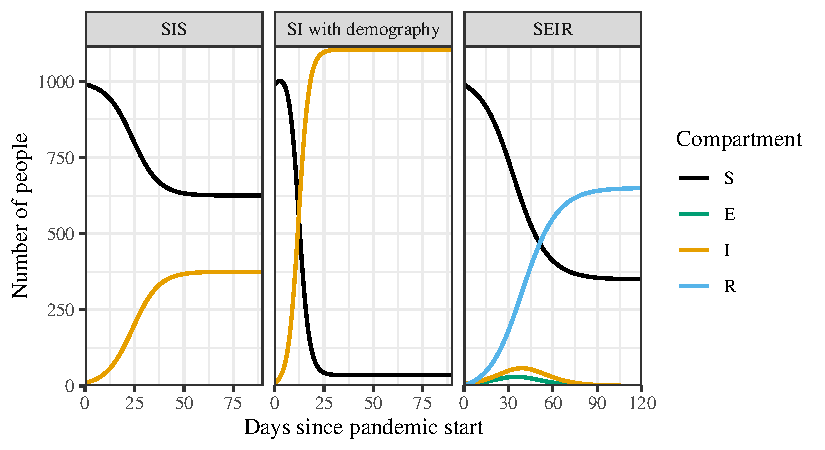
\includegraphics{ODE_plots.pdf}
    \caption{
        Solutions to the ordinary differential equations describing the models 
        depicted in Figure \ref{fig:simple_models}. The initial infectious 
        population was $I_0 = 10,$ with $S_0 = 990.$ In the $SEIR$ model, 
        $E_0 = R_0 = 0.$ For all models $\beta = 0.4.$ For the $SIS$ and $SI$
         model with demography $\gamma = 1/4.$ For the $SI$ model with 
         demography $\mu = 0.012,$ and $\nu = 0.0012.$ For the $SEIR$ model, 
         $\gamma = 1/90,$ and $\sigma = 1/2.$
    }
         \label{fig:ODE_outputs}
\end{figure}

After specifying the initial for each compartment the ordinary differential equations have a deterministic output, such as in \ref{fig:ODE_outputs}.

\section{Stochastic models}

\subsection*{Motivating the form of the stochastic model}

To establish a relationship between the deterministic and stochastic disease models, we first need to establish Poisson point processes and their properties.

\begin{definition}[Poisson Point Process]\label{def:ppp}
    $\{\N(t)\}_{t\geq0}$ is a \emph{(stationary) Poisson point process} with intensity $\lambda$ if \begin{enumerate}
        \item $\N(0) = 0$
        \item $\N(t_1) - \N(t_0), \N(t_2) - \N(t_1), \dots, \N(t_n) - \N(t_{n-1})$ are independent for $0 \leq t_0 < t_1 < \dots < t_{n-1} < t_n $
        \item $\N(t_2) - \N(t_1) \sim \Pois(\lambda(t_2 - t_1)), 0 \leq t_1 < t_2.$
    \end{enumerate}
\end{definition}

Deterministic ODE models are appropriate to study a kind of aggregate disease spread behaviour, and well approximate real world behaviour when the numbers in each compartment are large, however at the start of an epidemic, when the number of infected individuals is small the behaviour of the epidemic may vary significantly. It is possible that if the average number of people that an infectious individual infects near the beginning of the epidemic (formally referred to as $R_0$) is close to 1, then the disease may die out or become stable. Under the deterministic $SIS$ model described by equations \ref{eq:SIS_1} and \ref{eq:SIS_2}, consider the model at time $t^*$ the instantaneous rate at which $S$ is decreasing is $\beta \frac{I_{t^*}}{N} S_{t^*}.$ In other words, one individual leaves the $S$ compartment every $\beta \frac{I_{t^*}}{N} S_{t^*}$ units of time. We can consider a Poisson point process $\{\N_1(t - t^*)\}_{t\geq t^*}$ with intensity $\beta \frac{I_{t^*}}{N} S_{t^*}$ corresponding to the count of the number of individuals who have left $S$ and entered $I$ $t$ units of time since $t^*.$ $$\frac{\diff \E(\N_1(t^*))}{\diff t^*} = \lim_{\delta \to 0}\frac{\E{(\N(t^* + \delta) - \N(t^*))}}{\delta} = \frac{\beta \frac{I_{t^*}}{N} S_{t^*}(t^* + \delta - t^*)\beta \frac{I_{t^*}}{N} S_{t^*}}{\delta} = \beta \frac{I_{t^*}}{N} S_{t^*}.$$

Under the same deterministic formulation of the model, the instantaneous rate into $S$ at $t^*$ is $\gamma I_{t^*}.$ Therefore as above we can construct a Poisson point process $\{\N_2(t - t^*)\}_{t\geq t^*}$ with rate $\gamma I_{t^*}$ describing the number of recoveries from $I$ to $S,$ with $\frac{\diff \E(\N_2(t^*))}{\diff t^*} = \gamma I_{t^*}.$ Combining the two processes, we can see that the rate of change in the average number of people in $S$ is $$\frac{\diff \E(\N_2(t^*) - \N_1(t^*))}{\diff t^*} = \frac{\diff \E(\N_2(t^*)) - \diff \E(\N_1(t^*))}{\diff t^*} = -\beta \frac{I_t}{N}S_t + \gamma I = \frac{\diff S_t}{\diff t}.$$

% \begin{definition}[Markov Chain]
%     A set of random variables $\{X_i\}_{i\in\mathcal{I}}$ is Markov if $\Pr(X_{i})$
% \end{definition}

Therefore we can create a stochastic model where the local average in each compartment matches the behaviour of the ODE model at the same state. We do this first by formulating the model as a random vector $\{\mathbf{C}_t\}_{t\geq 0} = \{C_1(t), C_2(t), \dots, C_n(t)\}_{t\geq 0}$ where $C_i:\mathbb{R} \to \mathbb{N}\cup\{0\},$ is the number of people in compartment $C_i,$ and for any fixed $t$, $\{C_1(t), C_2(t), \dots, C_n(t)\}$ is a random variable describing the state of the model. For example in a model with $S$ and $I$ compartments, $\{\mathbf{C}_t\}_{t\geq 0}:=\{S_t, I_t\}_{t\geq 0}.$ $\{\mathbf{C}_t\}_{t\geq 0}$ is a continuous time Markov chain (see Definition \ref{Markov_chains}) with transition kernel corresponding to the rates of the model. For example, in the $SI$ model with demography in Figure \ref{fig:SI_demog_model} the transition rates are: \begin{itemize}
    \item $\{s, i\}$ to $\{s + 1, i\}$ has rate $\mu (s + i)$
    \item $\{s, i\}$ to $\{s - 1, i\}$ has rate $\nu s$
    \item $\{s, i\}$ to $\{s - 1, i + 1\}$ has rate $\beta \frac{i}{i+s}s$
    \item $\{s, i\}$ to $\{s, i - 1\}$ has rate $(\nu + \gamma) i.$
\end{itemize}

We can interpret each transition as a seperate events, each behaving as independent Poisson point processes until the time of the first transition. Therefore at time $t^*$ we have the Poisson point processes: \begin{itemize}
    \item $\{\mathcal{E}_1(t)\}_{t\geq 0}:$ the number of births into $S$ after time $t^*$ with intensity $\mu N_{t^*}$
    \item $\{\mathcal{E}_2(t)\}_{t\geq 0}:$ the number of deaths in $S$ after time $t^*$ with intensity $\nu S_{t^*}$
    \item $\{\mathcal{E}_3(t)\}_{t\geq 0}:$ the number of infections after time $t^*$ with intensity $\beta \frac{I_{t^*}}{N_{t^*}} S_{t^*}$
    \item $\{\mathcal{E}_4(t)\}_{t\geq 0}:$ the number of deaths from $I$ after time $t^*$ with intensity $(\nu + \gamma) I_{t^*}.$
\end{itemize}

\begin{theorem}[Sums of Independent Poisson Point Processes]\label{thm:sum_ppp}
    Given independent Poisson point processes $\{\N_1(t)\}_{t\geq0},
        \{\N_2(t)\}_{t\geq0}, \dots,  \{\N_n(t)\}_{t\geq0},$ with intensities
    $\lambda_1, \lambda_2, \dots, \lambda_n,$
    $$\{\N(t)\}_{t\geq0} := \{\N_1(t) + \N_2(t) + \dots + \N_n(t)\}_{t\geq0}$$ is a Poisson point process with intensity $\lambda_1 + \lambda_2 + \dots +
        \lambda_n.$
\end{theorem}

\begin{proof}
    We show that
    $\{\N(t) := \{\N_1(t) + \N_2(t) + \dots + \N_n(t)\}_{t\geq0}\}$ meets each
    component of Definition \ref{def:ppp}.
    \begin{enumerate}
        \item $\N(0) := \N_1(0) + \N_2(0) + \dots + \N_n(0) = 0$ since
              $\N_i(0) = 0$ by definition of a Poisson point process.
        \item We show that $\N(t_1) - \N(t_0), \N(t_2) - \N(t_1), \dots,
                  \N(t_n) - \N(t_{n - 1})$
              with $0 \leq t_0 < t_1 < \dots < t_n$ are independent.
              $$\N(t_i) - \N(t_{i - 1})
                  = \underset{X_{i1}}
                  {\underbrace{[\N_1(t_i) - \N_1(t_{i - 1})]}}
                  + \underset{X_{i2}}
                  {\underbrace{[\N_2(t_i) - \N_2(t_{i - 1})]}} + \dots
                  + \underset{X_{in}}
                  {\underbrace{[\N_n(t_i) - \N_n(t_{i - 1})]}}$$
              $X_{ik}$ is independent of $X_{j\ell}$ for $k \neq \ell$ since
              $\N_k$ and $\N_\ell$ are independent processes. $X_{ik}$ is
              independent of $X_{jk}$ for $i\neq j$ by the second property
              of Definition \ref{def:ppp}. Therefore all $X_{ik}$ are
              independent of $X_{j\ell}$ for $i\neq j,$ and all $j, k.$
              Hence
              $\N(t_1) - \N(t_0), \N(t_2) - \N(t_1), \dots,
                  \N(t_n) - \N(t_{n - 1})$
              with $0 \leq t_0 < t_1 < \dots < t_n$ are independent.
        \item For fixed $t_1 < t_2,$ and $i \in \{1, 2, \dots, n\},$
              $$\N_i(t_2) - \N_i(t_1) \sim \Pois((t_2 - t_1)\lambda_i).$$
              Consider the associated moment generating function of
              $\N_i(t_2) - \N_i(t_1),$
              $$M_i(z) := \exp(\lambda_i(t_2 - t_1)(\exp(z) - 1)).$$
              Therefore the moment generating function of
              $$\N(t_2) - \N(t_1) =
                  [\N_1(t_2) - \N_1(t_1)] + [\N_2(t_2) - \N_2(t_1)] + \dots
                  + [\N_n(t_2) - \N_n(t_1)]$$ is
              $$ M(z) := \prod_{i = 1}^n M_i(z) =
                  \exp[
                      (\lambda_1 (t_2 - t_1) + \lambda_2 (t_2 - t_1) + \dots
                      + \lambda_n (t_2 - t_1))
                      (\exp(z) - 1)
                  ].$$
              Therefore
              $\N_1(t) + \N_2(t) + \dots + \N_n(t) \sim
                  \Pois((\lambda_1 + \lambda_2 + \dots + \lambda_n) t)$
              by the uniqueness of the moment generating function.
    \end{enumerate}
\end{proof}

\begin{theorem}[Time to First Event in Poisson Point Process]
    \label{thm:next_pp_event}
    Given a Poisson point process $\{\N(t)\}_{t\geq 0}$ with intensity
    $\lambda,$ let $\tau = \inf\{t | \N(t_0 + t) - \N(t_0) = 1, t > 0\}$.
    $\tau \sim \Exp(\lambda)$ for $t_0 \geq 0$
\end{theorem}

\begin{proof}
    $$\Pr(\tau > x) = \Pr(\N(t_0 + x) - \N(t_0) = 0)
        = \frac{(\lambda x)^0e^{-\lambda x}}{0!} = e^{-\lambda x}$$
\end{proof}

By Theorem \ref{thm:sum_ppp} and Theorem \ref{thm:next_pp_event},
$$\{\mathcal{E}(t)\}_{t\geq 0}:=\{\mathcal{E}_1(t) + \mathcal{E}_2(t)
    + \mathcal{E}_3(t) + \mathcal{E}_4(t)\}_{t\geq 0}$$
is a Poisson point process with intensity
$$\mu N_{t^*} + \nu S_{t^*} + \beta \frac{I_{t^*}}{N_{t^*}} S_{t^*}
    + (\nu + \gamma) I_{t^*},$$
and the time to the next event is random variable distributed
$$\Exp(\mu N_{t^*} + \nu S_{t^*}
    + \beta \frac{I_{t^*}}{N_{t^*}} S_{t^*} + (\nu + \gamma) I_{t^*}).$$

\begin{theorem}[Probability of $i$th Poisson Process Generating the Next Event]\label{thm:which_ppp}
    Consider independent Poisson point processes
    $$\{\N_1(t)\}_{t\geq0},\, \{\N_2(t)\}_{t\geq0},\, \dots,\,
        \{\N_n(t)\}_{t\geq0}$$
    having intensities $\lambda_1, \lambda_2, \dots, \lambda_n.$ For fixed
    $t_0,$ let $\tau_i:=\inf\{t | \N(t_0 + t) - \N(t_0) = 1\}.$
    Then
    $$\Pr(\min_i{\tau_i} = \tau_j)
        = \frac{\lambda_j}{\sum_{i = 1}^n \lambda_i}.$$
\end{theorem}
\begin{proof}
    By Theorem \ref{thm:next_pp_event}, $\tau_i \sim \Exp(\lambda_i).$
    Therefore \begin{align*}
        \Pr(\min_i{\tau_i} = \tau_j) = & \int_0^\infty \Pr(\{\tau_i = x\} \cup \bigcup_{j\neq i}\{\tau_j > x\}) \diff x                    \\
        =                              & \int_0^\infty \Pr(\{\tau_i = x\} \cup \bigcup_{j\neq i}\{\tau_j > x\}) \diff x                    \\
        =                              & \int_0^\infty \Pr(\tau_i = x)\times \prod_{j\neq i}\Pr(\tau_j > x) \diff x\tag{by independence}   \\
        =                              & \int_0^\infty \lambda_i\exp(-\lambda_i x) \times \prod_{j\neq i}\exp(-\lambda_j x) \diff x        \\
        =                              & \lambda_i\int_0^\infty \exp(-(\sum_{i = 1}^n\lambda_j) x) \diff x                                 \\
        =                              & \lambda_i\left[\frac{\exp(-(\sum_{i = 1}^n\lambda_j) x)}{\sum_{i = 1}^n\lambda_j}\right]_0^\infty \\
        =                              & \frac{\lambda_i}{\sum_{i = 1}^n\lambda_j}
    \end{align*}
\end{proof}

\section{Doob-Gillespie Algorithm}

All of this leads naturally to a common method of simulating the stochastic model. The Doob-Gillespie algorithm (often just called the Gillespie algorithm) is an algorithm that simulates a stochastic realisation of a model given a set of starting conditions.

\begin{algorithm}
    \caption{The Doob-Gillespie Algorithm}\label{alg:doob}
    \begin{algorithmic}[1]
        \State Initialise time $t \gets 0$ and initial state of the model $\mathbf{C}(0) := \{C_1(0), C_2(0), \dots, C_n(0)\}$
        \While{termination condition not met}
        \State Calculate intensities $\lambda_i$ for all possible events $\mathcal{E}_i$
        \State Calculate total intensity $\lambda = \sum_i \lambda_i$
        \State Generate $\Delta t \sim \Exp(\lambda)$
        \State Choose event $\mathrm{E}_i$ with probability $\frac{\lambda_i}{\lambda}$
        \State Update time $t \gets t + \Delta t$
        \State Update state of $\mathbf{C}(t + \delta t) \gets \mathbf{C}(t) + \text{ change in state due to event } \mathcal{E}_i$
        \EndWhile
    \end{algorithmic}
\end{algorithm}

\begin{figure}[htbp]
    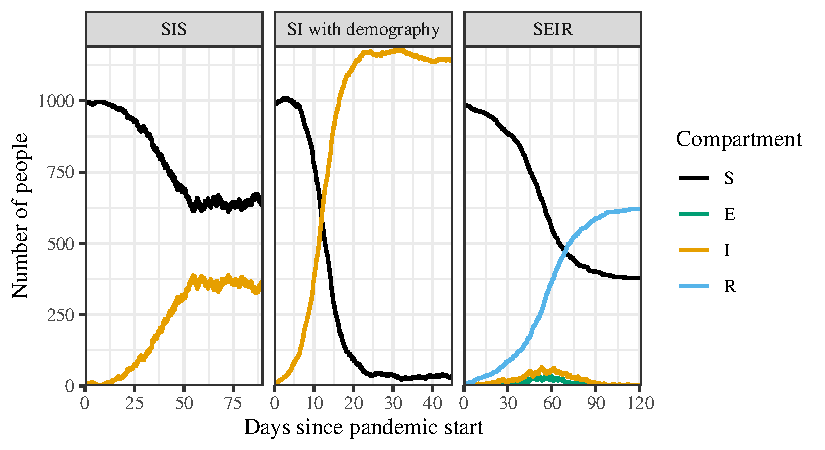
\includegraphics{doob_plots.pdf}
    \caption{Exact stochastic simulations of the 3 different models using Algorithm \ref{alg:doob}. The parameters used were identical to those in Figure \ref{fig:ODE_outputs}}\label{fig:doob_outputs}
\end{figure}

\section{\texorpdfstring{$\tau$}{Lg}-leaping}

$\tau$-leaping exploits the local Poisson point process like behaviour of epidemiological models. Consider the SIS model, when $S_t = I_t = 10000.$ Events happen at a very high rate, meaning the $\Delta t$ found in each step of the Doob-Gillespie algorithm will be very small, but the rates also change a negligible amount after each event (compare $\gamma\times 10000$ to $\gamma\times 10001$ or $\gamma\times 9999$). Therefore we can approximate the number of events in a short time period $\tau$ as a Poisson point process with the total intensity $\lambda = \sum_i \lambda_i$ at time $t,$ with the probability of any one event having the same probability as above of $\frac{\lambda_i}{\lambda}.$ Therefore we have the following algorithm.

\begin{algorithm}
    \caption{$\tau$-Leaping Algorithm}
    \label{alg:tau_leaping}
    \begin{algorithmic}[1]
        \State Initialise time $t \gets 0$ and initial state of the model $\mathbf{C}(0) := \{C_1(0), C_2(0), \dots, C_n(0)\}$
        \While{termination condition not met}
        \State Calculate intensities $\lambda_i$ for all possible events $\mathcal{E}_i$
        \State Calculate total intensity $\lambda = \sum_i \lambda_i$
        \State Choose a suitable time step $\tau$ (this can be deterministic or adaptive)
        \State Calculate Poisson random variable $X \sim \text{Poisson}(\lambda)$
        \For{$i$ in 1 to $X$}
        \State Choose event $\mathrm{E}_i$ with probability $\frac{\lambda_i}{\lambda}$
        \State Update state of $\mathbf{C}(t + \tau) \gets \mathbf{C}(t) + \text{ change in state due to event } \mathcal{E}_i$
        \EndFor
        \State Update time $t \gets t + \tau$
        \EndWhile
    \end{algorithmic}
\end{algorithm}

% \section{Individual based models}
% \chapter{Malaria and Malaria Models}

\section{Malaria}

Malaria kills around 600,000 people each year, with over 75\% of deaths
occuring in children under 5 years old
\parencite{world_health_organization_world_2022}.

\subsection*{Plasmodium Life Cycle}

\begin{figure}[htbp]
    \missingfigure{Eamon how do I use the biorender thing?}
    \caption{The malaria lifecycle.}\label{fig:mal_lc}
\end{figure}

Malaria is a vector borne disease, needing both human (or other vertebrate) and
mosquito hosts to complete it's lifecycle (Figure \ref{fig:mal_lc}). Six
species of the unicellular parasite able to infect humans
\parencite{milner_malaria_2018}. Although \textit{Plasmodium falciparum} is
responsible for around 90\% of total human malaria deaths, outside of Africa
\textit{Plasmodium vivax} is the leading cause of malaria infection
\parencite{zekar_plasmodium_2023, adams_biology_2017}. Sporozoites (a stage of
the malaria parasite) enter the human blood stream via the skin after the
female mosquito has a blood meal. From the blood stream they proceed to enter
into the liver. Once a hepatocyte (liver cell) is invaded, the parasite will
undergo asexual reproduction into up to 40,000 merozoites per hepatocyte, which
are released into the blood stream . These merozoites then bind to, and invade
erythrocytes (red blood cells), once again reproducing 16-32 fold in a process
called schizogony. At this point, the erythrocyte membrane is ruptured,
allowing for \textit{Plasmodium} to invade new erythrocytes. Eventually, the
merozoites undergo sexual differentiation, resulting in the sequestration and
maturation of male and female gametocytes in the bone marrow, until they are
released into the blood stream to be consumed by a mosquito during a blood feed
where it matures into sporozoites ready to reinfect a new vertebrate host when
the mosquito next takes a blood feed \parencite{cowman_malaria_2016}.

\subsection*{Illness, Treatment, and Immunity}

The most common symptom of malaria infection in persons without natural or
acquired immunity is fever. After treatment, fever will usually subside over a
few days. In severe cases, malaria can lead to anemia, cerebral malaria (coma),
and respiratory distress \parencite{cowman_malaria_2016}.

In a population with stable malarial infection, immunity increases with age,
with the proportion of severe cases negligible after age 10, and asymptomatic
infection being the dominant infection type beyond age 15
\parencite{cowman_malaria_2016}.

\subsection*{Control and Eradication}

Widespread use of DDTs in the mid 20th century led to significant successes in
some countries towards the control and eradication of malaria. In the 1980s and
1990s, drug resistant malaria led to a doubling of malaria-attributable death.
Currently, the control techniques include insecticide treated bed nets, and a
mixture of antimalarial drugs \parencite{cowman_malaria_2016}.

\subsection*{\textit{Plasmodium vivax}}

Unlike \textit{P.\ falciparum}, \textit{P.\ vivax} has hypnozoites, which are a
dormant liver stage of the parasite. These can remain dormant for weeks and
even months, leading to recurrent infections and illness, possibily until the
conditions for transmission are more favourable. In subtropical/temperate
areas, the incubation periods can be between 8-12 months, compared to 3-4 weeks
in tropical regions. \cite{price_plasmodium_2020}. \textit{P.\ vivax} also has
lower levels of the blood stage parasite during infection, which means
diagnosis is more difficult, and it has an increased proportion of asymptomatic
cases \parencite{adams_biology_2017}.

It is likely that death and severe disease attributable to \textit{P.\ vivax}
has been traditionally underestimated. In view of recent evidence, the old
notion that \textit{P.\ vivax} is benign has become untenable
\parencite{cowman_malaria_2016}.

\subsection*{Motivating Malaria Models}

Levels of asymptomatic cases and latent parasite (in the case of
\textit{P.\ vivax}) are impossible or difficult to experimentally determine
without mass testing. By creating a model of the disease, and calibrating the
model so that it simulates symptomatic case levels reported by health
authorities, it is possible to estimate these previously `hidden' levels.
Furthermore, modelling malaria allows for modelling the effect of public health
interventions such as mass treatment or testing, in order to determine an
estimate of how effective the intervention may be, before large amounts of
money are spent on trials.

\section{Malaria Models}

\subsection*{Ross-Macdonald}

\begin{figure}[htbp]
    \centering
    \begin{tikzpicture}[thick]
        \node[draw, minimum size=1.5cm] (SH) {$S_\mathrm{H}$};
        \node[draw, right=of SH, minimum size=1.5cm] (IH) {$I_\mathrm{H}$};
        \node[draw, below=of SH, minimum size=1.5cm] (SM) {$S_\mathrm{M}$};
        \node[draw, below=of IH, minimum size=1.5cm] (IM) {$I_\mathrm{M}$};
        \draw[->] (SH) edge node [midway, label=above:{$\lambda_\mathrm{H}$}] (lambdaH) {} (IH);
        \draw[->] (SM) edge node [midway, label=below:{$\lambda_\mathrm{M}$}] (lambdaM) {} (IM);
        \draw[->, dashed, ruby] (IH) to (lambdaM);
        \draw[->, dashed, ruby] (IM) to (lambdaH);
        \draw[->] (IH) edge[in = 90, out = 90] node [midway, label=above:{$\gamma_\mathrm{H}$}] (omegaH) {} (SH);
        \node[below=of SM] (b_SM) {};
        \node[left=of SM] (l_SM) {};
        \node[below=of IM] (b_IM) {};
        \draw[->] (SM) edge node [midway, label=right:{$\mu_M$}] (SmuM) {} (b_SM);
        \draw[->] (l_SM) edge node [pos = 0.1, label=above:{$N_M\mu_M$}] (NmuM) {} (SM);
        \draw[->] (IM) edge node [midway, label=right:{$\mu_M$}] (ImuM) {} (b_IM);
    \end{tikzpicture}
    \caption{A simple Ross-Macdonald malaria model schematic, as described by \cite{aron_population_1982}. $S_\mathrm{H}$ and $I_\mathrm{H}$ are the number of susceptable and infected humans respectively, and $S_\mathrm{M}$ and $I_\mathrm{M}$ are the number of susceptable and infected mosquitos. The rate of human infection ($\lambda_\mathrm{H}$) is dependant on $I_\mathrm{M}$, and the rate of human infection ($\lambda_\mathrm{M}$) is dependant on $I_\mathrm{H}$.}\label{fig:ross_mac}
\end{figure}

Modelling malaria presents an additional challenge, as the disease is transmitted from mosquito to human and human to mosquito, rather than having direct human to human transmission. The most simple Ross-Macdonald model is depicted in figure \ref{fig:ross_mac}. The ODEs for this model are \begin{align*}
    \frac{\diff S_\mathrm{H}}{\diff t} = & \, \gamma_\mathrm{H}I_\mathrm{H} - bT_{\mathrm{HM}}I_\mathrm{M}\frac{S_\mathrm{H}}{N_\mathrm{H}}                                         \\
    \frac{\diff I_\mathrm{H}}{\diff t} = & \, bT_{\mathrm{HM}}I_\mathrm{M}\frac{S_\mathrm{H}}{N_\mathrm{H}} - \gamma I_\mathrm{H}                                                   \\
    \frac{\diff S_\mathrm{M}}{\diff t} = & \, N_\mathrm{M}\mu_M + \gamma_\mathrm{M}I_\mathrm{M} - bT_{\mathrm{MH}}S_\mathrm{M}\frac{I_\mathrm{H}}{N_\mathrm{H}} - S_\mathrm{M}\mu_M \\
    \frac{\diff I_\mathrm{M}}{\diff t} = & \, bT_{\mathrm{MH}}S_\mathrm{M}\frac{I_\mathrm{H}}{N_\mathrm{H}} - \gamma_\mathrm{M}I_\mathrm{M}
\end{align*} where $b$ is the biting rate per mosquito, and $T_{\mathrm{HM}}$ is the probability of tranmission to a human given a bite by an infectious mosquito, with $T_{\mathrm{MH}}$ being vice-versa. Note that it is $\frac{I_\mathrm{H}}{N_\mathrm{H}}$ in the mosquito dynamics. Biologically this is assuming the number of blood meals a mosquito takes per day is invariant to the size of the human population. Mosquitos don't `recover' from malaria due to their short lifespans, but the births and deaths are mathematically equivalent to assuming that the rate of `recovery' amongst mosquitos is $\mu_\mathrm{M}I_\mathrm{M}$ per unit time, with no population dynamics.

A Ross-Macdonald style model simplifies the lifecycle of malaria to the following four steps \parencite{smith_ross_2012}: \begin{enumerate}
    \item Malaria is transmitted to human (or vertebrate) via a blood feed.
    \item Malaria proliferates in the human host until it circulates in the peripheral blood
    \item A mosquito then takes a blood feed, ingesting the pathogen
    \item Malaria develops within the mosquito host, progressing to its salivary glands, able to infect a human.
\end{enumerate}

\subsection*{Models of \textit{P.\ Vivax} Malaria}

\subsubsection*{White Model}

\begin{figure}[htbp]
    \centering
    \begin{tikzpicture}[thick]
        \node[draw, minimum size=1cm] (S0) {$S_0$};
        \node[draw, right of=S0, minimum size=1cm, node distance=3.5cm] (I0) {$I_0$};
        \node[draw, below of=S0, minimum size=1cm, node distance=3.5cm] (SL) {$S_\mathrm{L}$};
        \node[draw, below of=I0, minimum size=1cm, node distance=3.5cm] (IL) {$I_\mathrm{L}$};
        \node[draw, right of=I0, minimum size=1cm, node distance=3.5cm] (SM) {$S_\mathrm{M}$};
        \node[draw, right of=IL, minimum size=1cm, node distance=3.5cm] (IM) {$I_\mathrm{M}$};
        \draw[->] (S0) edge node [midway, label=above:{$\lambda_\mathrm{H}$}] (lambdaH1) {} (IL);
        \draw[->] (SL) edge node [midway, label=left:{$\gamma_\mathrm{L}$}] (gammaL1) {} (S0);
        \draw[->] (SL) edge[in = 170, out = 10] node [midway, label=above:{$\lambda_\mathrm{H} + f$}] (lambdaf) {} (IL);
        \draw[->] (IL) edge[in = -10, out = 190] node [midway, label=below:{$r$}] (r) {} (SL);
        \draw[->] (IL) edge[in = 260, out = 100] node [midway, label=left:{$\gamma_\mathrm{L}$}] (gammaL2) {} (I0);
        \draw[->] (I0) edge[in = 80, out = 280] node [midway, label=right:{$\lambda_\mathrm{H}$}] (lambdaH2) {} (IL);
        \draw[->] (I0) edge node [midway, label=above:{$r$}] (r2) {} (S0);
        \draw[->] (SM) edge node [midway, label=left:{$\lambda_\mathrm{M}$}] (lambdaM) {} (IM);
    \end{tikzpicture}
    \caption{Diagram for \textit{P.\ vivax} model in a tropical setting described by \cite{white_variation_2016}. $S$ and $I$ are the number of susceptable and infected humans and mosquitos (denoted by subscript M). $\lambda_\mathrm{H} = mabI_\mathrm{M}$ and $\lambda_\mathrm{M} = ac(I_0 + I_\mathrm{L})$}\label{fig:white_2}
\end{figure}

The White model - described in \cite{white_variation_2016} (tropical model) and depicted in Figure \ref{fig:white_2} - is characterised by the following ordinary differential equations:

\begin{align*}
    \frac{\diff S_0}{\diff t} =          & -\lambda_\mathrm{H} S_0 + rI_0 + \gamma_\mathrm{L}S_\mathrm{L}                                                                            \\
    \frac{\diff I_0}{\diff t} =          & -\lambda_\mathrm{H} I_0 - rI_0 + \gamma_\mathrm{L}I_\mathrm{L}                                                                            \\
    \frac{\diff S_\mathrm{L}}{\diff t} = & -\lambda_\mathrm{H} S_\mathrm{L} + rI_\mathrm{L} - fS_\mathrm{L} -\gamma_\mathrm{L}S_\mathrm{L}                                           \\
    \frac{\diff I_\mathrm{L}}{\diff t} = & \lambda_\mathrm{H} (S_0 + I_0 + S_\mathrm{L}) - rI_\mathrm{L} + fS_\mathrm{L} -\gamma_\mathrm{L}I_\mathrm{L}                              \\
    \frac{\diff S_\mathrm{M}}{\diff t} = & g - \lambda_\mathrm{M}(pS_\mathrm{M} - (1 - p)I_\mathrm{M}) - gS_\mathrm{M}                                                               \\
    \frac{\diff I_\mathrm{M}}{\diff t} = & \lambda_\mathrm{M}(pS_\mathrm{M} - (1 - p)I_\mathrm{M}) - gI_\mathrm{M}\tag{$I_0 + I_\mathrm{L}=$ total number of bloodstage infections}.
\end{align*}

It modifies the Ross-Macdonald models, to capture the differences in disease progression between \textit{P.\ vivax} and \textit{P.\ falciparum}. In particular, the White model includes the dormant liver stage that is unique to \textit{P.\ vivax}.

The model is comprised of six compartments: \begin{enumerate}
    \item \textbf{$S_0$ (Susceptible Individuals - No Latent Hypnozoite Liver Stage Infection)}: People in this compartment have no form of malarial infection. These people are susceptible to new malarial infections, and are infected into compartment $I_\mathrm{L}$ (with both blood and liver stage parasites) with rate $\lambda_\mathrm{H}$.
    \item \textbf{$I_\mathrm{L}$ (Infected Individuals - Both Blood Stage and Latent Hypnozoite Liver Stage Infection)}:  Individuals in this compartment have both an active blood-stage infection, and latent hypnozoite infection in the liver. They can progress to either $I_0$ through the clearance of liver stage infection with rate $\gamma_\mathrm{L},$ or to $S_\mathrm{L}$ through clearance of blood stage infection with rate $r$.
    \item \textbf{$I_0$ (Infected Individuals - Blood-Stage Infection Only)}: Those in this compartment have a blood-stage infection with no latent hypnozoite infection in the liver. They are be reinfected into $I_\mathrm{L}$ with rate $\lambda_\mathrm{H}$, relapse with rate $f$. Blood-stage infection is cleared (moving into compartment $S_0$) with rate $r$.
    \item \textbf{$S_\mathrm{L}$ (Susceptable Individuals - Blood-Stage Infection Only)}: Those in this compartment have latent hypnozoite infection in the liver without blood-stage infection. They get novel infection through a mosquito bite into $I_\mathrm{L}$ with rate $\lambda_\mathrm{H}$, or hypnozoite activation with rate $f$. This means that those in $S_\mathrm{L}$ move to compartment $I_\mathrm{L}$ with total rate $\lambda_\mathrm{H} + f.$ Alternatively the hypnozoites are cleared from the liver (moving to compartment $S_0$) with rate $\gamma_\mathrm{L}.$
    \item \textbf{$S_\mathrm{M}$ (Susceptable Mosquitoes)}: Suspectable mosquitoes become infectious at rate $\lambda_\mathrm{M}p.$ They die at rate $g + \lambda_\mathrm{M}(1 - p).$ Since there is a constant mosquito population assumption, mosquitoes are born into this state at rate $g + \lambda_\mathrm{M}.$
    \item \textbf{$I_\mathrm{M}$ (Infectious Mosquitoes)}: Infectious mosquitos die at rate $g + \lambda_\mathrm{M}(1 - p).$
\end{enumerate}

$\lambda_\mathrm{H} := mabI_\mathrm{M}$ where $m$ is the number of mosquitos per human (held constant since there is no birth or death in the human dynamics), $a$ is the mosquito biting rate, and $b$ is the probability that a human bitten by an infectious mosquito develops an infection.

$\lambda_\mathrm{M} := ac(I_0 + I_\mathrm{L})$ where $a$ is defined above, and $c$ is the probability that a mosquito bite on an infectious mosquito causes the mosquito to become infectious. $g$ can be interpreted as the natural birth/death rate for mosquitos. $p$ is then the proportion of mosquitos that survive long enough after the initial infection that the parasite matures enough in the mosquito before becoming infectious to new susceptible humans. Under the assumption that time until parasite transmissability after infection in a mosquito is a constant $n$ days, and that mosquitoes naturally die at rate $g$, $p=e^{-gn}.$ To see this let $V\sim\mathrm{Exp}(g),$ represent the lifespan of the mosquito. $\Pr(V > n)= 1 - F_V(n) = 1 - (1 - e^{-gn}) = e^{-gn}.$

$\lambda_\mathrm{M}(1 - p)$ can be interpreted as an additional rate of death, where of the mosquitos that would develop malaria after a bite, a proportion $1 - p$ die instantly. This applies to both the susceptible and infectious mosquitoes. Presumably this approximates a model where mosquitoes are moved to an `exposed' compartment for $n$ time, after initial infection, however no justification is given in \parencite{white_variation_2016} for this additional parameter $n$. A more straightforward $SI$ model could be constructed that absorbs $c$ and $n$ into the single parameter $c^*$, such that it becomes the proportion of mosquito bites on blood stage infectious humans that result in mosquito infection where the mosquito does not die before becoming infectious. With steady mosquito population, the mosquito dynamics would now be characterised by
$$\frac{\diff I_\mathrm{M}}{\diff t} = \lambda_\mathrm{M}^*S_\mathrm{M}- gI_\mathrm{M}\quad\text{where } \lambda_\mathrm{M}^*:= ac^*(I_0 + I_\mathrm{L}).$$

By modelling both liver and bloodstage infection, blood stage infections from relapses can be captured in the dynamics, meaning it is possible to analyse case number data that may be confounded by relapses as well as novel infections.

% Combining this model with pre-established within host dynamics, the model allows for analysis of how the hypnozoite activation rate (closely related to relapse frequency) can effect the total number of relapsing hypnozoites, the time with liver stage infection, and the basic reproduction number $R_0$ (important particularly in considering interventions and potential evolutionary strain selection).

This model does not account for continual depletion of liver stage parasites which would vary the rate of relapse over time (through clearance or relapse). It also does not directly model any interventions or case importations. The lack of population dynamics means the model may only be useful on a small time scale. Finally, it doesn't account for any importation of disease from an outside area, so if $S_0 = 1,$ \textit{P.\ vivax} is presumed permanently eradicated.

\subsubsection*{Champagne Model}

\begin{figure}[htbp]
    \centering
    \begin{tikzpicture}[thick]
        \node[draw, minimum size=1cm] (S0) {$S_0$};
        \node[draw, right of=S0, minimum size=1cm, node distance=7cm] (I0) {$I_0$};
        \node[draw, below of=S0, minimum size=1cm, node distance=7cm] (SL) {$S_\mathrm{L}$};
        \node[draw, below of=I0, minimum size=1cm, node distance=7cm] (IL) {$I_\mathrm{L}$};
        \draw[->] (S0) edge[sloped] node[above] {$(1 - \alpha)(\lambda I_\mathrm{total} + \delta)$} (IL);
        \draw[->] (S0) edge[in = 80, out = 280, sloped] node[above] {$\alpha( 1 -\beta)(\lambda I_\mathrm{total} + \delta)$} (SL);
        \draw[->] (SL) edge[in = 260, out = 100, sloped] node [above] {$\gamma_\mathrm{L} + \alpha\beta(\lambda I_\mathrm{total} + \delta + f)$} (S0);
        \draw[->] (SL) edge[in = 170, out = 10, sloped] node [above] {$(1 -\alpha)(\lambda I_\mathrm{total} + \delta + f)$} (IL);
        \draw[->] (IL) edge[in = -10, out = 190] node [midway, label=below:{$r$}] (r) {} (SL);
        \draw[->] (IL) edge[in = 260, out = 100, sloped] node [above] {$\gamma_\mathrm{L}$} (I0);
        \draw[->] (I0) edge[in = 80, out = 280, sloped] node [above] {$\lambda I_\mathrm{total} + \delta$} (IL);
        \draw[->] (I0) edge node [midway, label=above:{$r$}] (r2) {} (S0);
    \end{tikzpicture}
    \caption{Diagram for \textit{P.\ vivax} model described by \cite{champagne_using_2022}. $I_\mathrm{total} = I_0 + I _\mathrm{L}.$ Since the mosquito dynamics have been removed, $\lambda$ now not has no dependencies on the number of infectious mosquitos.}\label{fig:champ_diag}
\end{figure}

The Champagne model - described in \parencite{champagne_using_2022} and diagrammatically depicted in figure \ref{fig:champ_diag} - both simplifies and extends the White model. The model assumes human to human transmission, removing mosquito dynamics, and extends it by adding in a rate of imported cases and treatment of malarial infection. It is characterised by the system of ordinary differential equations
\begin{align*}
    \frac{\diff I_\mathrm{L}}{\diff t} = & (1 - \alpha)(\lambda I_\mathrm{total} + \delta)(S_0 + S_\mathrm{L}) + (\lambda I_\mathrm{total} + \delta)I_0 + (1 - \alpha)fS_\mathrm{L} - \gamma_\mathrm{L}I_\mathrm{L} - rI_\mathrm{L}  \\
    \frac{\diff I_0}{\diff t} =          & -(\lambda I_\mathrm{total} + \delta)I_0 + \gamma_\mathrm{L}I_\mathrm{L} - rI_0                                                                                                            \\
    \frac{\diff S_\mathrm{L}}{\diff t} = & -(1 - \alpha(1 - \beta))(\lambda I_\mathrm{total} + \delta + f)S_\mathrm{L} + \alpha(1-\beta)(\lambda I_\mathrm{total} + \delta)S_0 - \gamma_\mathrm{L}S_\mathrm{L} + rI_\mathrm{L}       \\
    \frac{\diff S_0}{\diff t} =          & -(1 - \alpha\beta)(\lambda I_\mathrm{total} + \delta)S_0 + (\lambda I_\mathrm{total} + \delta)\alpha\beta S_\mathrm{L} + \alpha\beta fS_\mathrm{L} + \gamma_\mathrm{L}S_\mathrm{L} + rI_0
\end{align*} where $I_\mathrm{total} := I_0 + I_\mathrm{L}.$

The compartments have the same interpretation as in the White model, however the rates between compartments are significantly modified.

The new parameters are $\lambda:$ the rate of infection, 
$\delta:$ importation rate, 
$\alpha:$ proportion of those infected who clear blood stage
infections through immediate treatment, and 
$\beta:$ proportion of those cleared of blood stage infection who
are also cleared of liver stage parasites (radical cure)
In other words, the proportion of infected individuals $\alpha\beta$ are 
completely cured from liver and blood stage parasites. The model assumes 
treatment clears infection instantaneously. Individuals in $S_\mathrm{L}$ who 
relapse or get a new infection are assumed to be cured with the same 
proportions as new infections from $S_0,$ but individuals in $I_0$ who are 
superinfected are assumed not to seek treatment.

In contrast to the White model, the Champagne model allows analysis of potential treatment interventions, or how much of an impact limiting the importation rate might have on case numbers (through border control/testing). Although the lack of mosquito dynamics simplifies the model and it's running, it is unrealistic. The model still has some of the same problems as the White model, such as not incorporating hypnozoite depletion rates and a lack of population dynamics, meaning all analytic results are done assuming the system is at equilibrium.
% \chapter{Parameter Inference}

\section{Motivation}

Building mathematical models of real world phenomenon allows for us to
simulate changes in the world without having to undertake large scale
experiments. However, once we have a model that sufficiently approximates
\emph{P. vivax} transmission
or anything else we are trying to model,
we then need to estimate what the `true' underlying parameters are.
To do this we calibrate the model against real world data such as case counts,
and prevalence surveys. Under frequentist assumptions, there is a `true' set of
parameters that if used in our model, simulated the observed data. Under a Bayesian
assumption, the parameters are considered to be random, and
This chapter explores statistical inference techniques to recover the
parameters, under both the frequentist and Bayesian frameworks.

\section{Frequentist Parameter Estimation}

Assume the model is parametrised by a set of parameters
$\btheta \in \mathbf{\Theta}$ which
we are trying to estimate by considering some observed data
$\by^\obs = (y_1^\obs, \dots, y_n^\obs).$
Consider $\by(\btheta) = (y_1(\btheta), \dots, y_n(\btheta))$
some model simulation of
$\by^\obs.$ Often the observed data has some underlying index set
$x_1, \dots, x_n,$ where $x_i$ might be something like time. In this case
we can also consider the observed data to be
$\{(x_1, y_1^\obs), \dots, (x_n, y_n^\obs)\},$ and the
model simulated data to be
$\{(x_1, y_1(\btheta)), \dots, (x_n, y_n(\btheta))\}.$

\subsection*{Least Squares Estimator}

It is common that models are not random, but instead model the mean behaviour
of a system. In this case, $\by(\btheta)$ is not random. Therefore
we can assume that $y^\obs_i = y_i(\btheta) + \varepsilon_i,$
where $\varepsilon_i$ is a random variable with some (possibly unknown)
distribution, and zero mean.

When the distribution of $\varepsilon_i$ is unknown, a common approach for
estimating $\btheta^{\LS}$ is to take the least squares estimate.

\begin{definition}[Least Squares Estimate]
    The \emph{least squares estimate} $\btheta^{\LS}$ for
    $\btheta$ is
    $$
        \btheta^{\LS}
        := \argmin_{\btheta\in\mathbf{\Theta}}
        \sum_{i = 1}^n (y_i(\btheta)- y_i^\obs)^2.
    $$
\end{definition}

\begin{example}\label{ex:LSE}
    Consider the observed data
    $\{(x_1, y_1^\obs), (x_2, y_2^\obs), (x_3, y_3^\obs)\}
        = \{(1, 2), (2, 4), (3, 4)\},$
    which we assume were generated from the model
    $y_i(\btheta) + \varepsilon_i,$ where
    $y_i(\btheta) = \theta_0 + \theta_1x_i,$ and
    $\E(\varepsilon_i) = 0.$ We derive the least squares estimate of our
    parameters $\btheta = (\theta_0, \theta_1)$ by

    \begin{align*}
        \btheta^{\LS}
        = & \, \argmin_{\btheta}
        [\sum_{i = 1}^3 (y_i(\btheta) - y_i^\obs)^2]           \\
        = & \, \argmin_{\btheta}
        [\sum_{i = 1}^3 (\theta_0 + \theta_1x_i - y_i^\obs)^2] \\
        = & \, \argmin_{\btheta}
        [(\theta_0 + \theta_1 - 2)^2 + (\theta_0 + 2\theta_1 - 4)^2
            + (\theta_0 + 3\theta_1 - 4)^2]
    \end{align*}

    Since the expanded quadratic will have positive coefficients out the front
    of $\theta_0$ and $\theta_1,$ we can solve for $\btheta^{\LS}$
    by

    \begin{align*}
        \mathbf{0}
        = & \, \frac{\partial}{\partial \btheta}
        [
            (\theta^\LS_0 + \theta^\LS_1 - 2)^2
            + (\theta^\LS_0 + 2\theta^\LS_1 - 4)^2
            + (\theta^\LS_0 + 3\theta^\LS_1 - 4)^2
        ]                                        \\
        = & \begin{bmatrix}
                6\theta^\LS_0 + 12\theta^\LS_1 - 20 \\
                12\theta^\LS_0 + 28\theta^\LS_1 - 44
            \end{bmatrix}
    \end{align*}
    And solving these two equations results in $\theta^\LS_0 = 4/3$ and
    $\theta^\LS_1 = 1.$ This can be visually seen in Figure \ref{fig:LSE}
\end{example}


\begin{figure}[htbp]
    \centering
    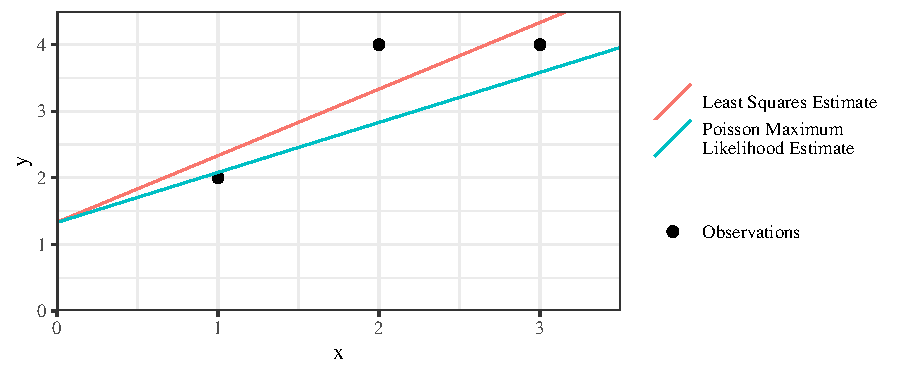
\includegraphics[width=\textwidth]{LS_example.pdf}
    \caption{
        Two linear models of the form
        $y_i(\btheta) = \theta_0 + \theta_1x_i$ fit given the set
        of observations $\{(1, 2), (2, 4), (3, 4)\}$ using the method of
        least squares and maximum likelihood under
        the assumption that the data are independent realisations by a Poisson
        distribution with $\Pois(y_i(\btheta)).$ The least squares estimates
        were $\theta^\LS_0 = 4/3$ and $\theta^\LS_1 = 1.$ The maximum likelihood
        estimates were $\hat{\theta}_0 \approx 1.329$ and
        $\hat{\theta}_1 \approx 0.751.$
    }
    \label{fig:LSE}
\end{figure}

\subsection*{Maximum Likelihood Estimator}

The least square method makes no explicit assumptions about the distribution
of the noise $\varepsilon.$ However if the distribution of $\varepsilon$ is
known (or can be reasonably assumed), we can
explicitly calculate the probability of the data given the parameters.

\begin{definition}[Likelihood function]
    With $\by^\obs$ fixed, the \emph{likelihood function} is
    $$
        \mathcal{L}(\btheta)
        := \Pr(
        \by(\btheta) + \bm{\varepsilon} = \by^\obs
        | \btheta
        ).
    $$
    Particularly, if $y_i(\btheta) + \varepsilon_i$ are independent
    $$
        \mathcal{L}(\btheta)
        = \prod_{i = 1}^n
        \Pr(
        y_i(\btheta) + \varepsilon_i = y_i^\obs
        | \btheta
        ).
    $$
\end{definition}

The dependence on $\by^\obs$ is suppressed, but can be
explicitly written as $\mathcal{L}(\btheta|\by^\obs).$ In the continuous
(and mixture of discrete and continuous) case,
we interpret
$
    \Pr(
    \by(\btheta) + \bm{\varepsilon} = \by^\obs
    | \btheta
    )
$
as the density
$
    \Pr(
    \by(\btheta) + \bm{\varepsilon} \in \diff\by^\obs
    | \btheta
    )
$ with respect to an underlying probability measure.

A natural estimate for $\btheta$ is the one that maximises the likelihood
function $\mathcal{L}$, as it coincides with the value of $\btheta$ maximises the
probability of the data. Such an estimate is called the maximum likelihood
estimate.

\begin{definition}[Maximum Likelihood Estimate]
    The \emph{maximum likelihood estimate} of $\btheta$ is
    $$
        \hat{\btheta}
        := \argmax_{\btheta\in\mathbf{\Theta}} \mathcal{L}(\btheta)
    $$
\end{definition}

It is often computationally easier to deal with the log-likelihood
$\ell(\btheta) := \ln\mathcal{L}(\btheta).$ Since $\ln$ is a monotonic function,
$\argmax_{\btheta\in\mathbf{\Theta}} \mathcal{L}(\btheta)
    = \argmax_{\btheta\in\mathbf{\Theta}} \ell(\btheta)$

\begin{example}
    Using the same observed data set as Example \ref{ex:LSE}, we assume that
    $y_i^\obs$ were generated independently from
    $y_i(\btheta) + \varepsilon_i \sim \Pois(y_i(\btheta)),$ where
    $y_i(\btheta) = \theta_0 + \theta_1x_i$ as previously defined. Therefore
    the maximimum likelihood estimate of $\btheta$ is
    \begin{align*}
        \hat{\btheta}
        = & \, \argmax \ell(\btheta)                                  \\
        = & \, \argmax_{\btheta\in\mathbf{\Theta}}\sum_{i = 1}^{3}
        y_i^\obs\ln(y_i(\btheta)) -y_i^\obs(\btheta) - \ln(y_i^\obs!) \\
        = & \, \argmax_{\btheta\in\mathbf{\Theta}}\sum_{i = 1}^{3}
        y_i^\obs\ln(\theta_0 + \theta_1x_i)
        - \theta_0 - \theta_1x_i
        - \ln(y_i^\obs!)                                              \\
        = & \, \argmax_{\btheta\in\mathbf{\Theta}}
        2\ln(\theta_0 + \theta_1) - \theta_0 - \theta_1
        + 4\ln(\theta_0 + 2\theta_1) - \theta_0 - 2\theta_1
        + 4\ln(\theta_0 + 3\theta_1) - \theta_0 - 3\theta_1
    \end{align*}
    which we numerically solve to get $\hat{\theta}_0 \approx 1.329$
    and $\hat{\theta_1} \approx 0.751,$ as seen in Figure \ref{fig:LSE}.
\end{example}

\subsection*{Relationship of Least Squares and Maximum Likelihood Estimates}

Although the least squares estimate does not explicitly assume a distribution,
it coincides with the maximum likelihood estimate under the assumption that
the $y_i^\obs$s were has been generated with normal error.

\begin{theorem}
    If $y_i(\btheta) + \epsilon_i \sim N(y_i(\btheta), \sigma^2),$ then
    $$
        \hat{\btheta} = \btheta^\LS
    $$
\end{theorem}

\begin{proof}
    \begin{align*}
        \hat{\btheta}
        = & \, \argmax_{\btheta\in\mathbf{\Theta}}\ell(\btheta) \\
        = & \, \argmax_{\btheta\in\mathbf{\Theta}}
        \sum_{i = 1}^n
        \ln(\frac{1}{\sqrt{2\pi}\sigma})
        -\frac{(y_i(\btheta)- y_i^\obs)^2}{\sigma^2}            \\
        = & \argmax_{\btheta\in\mathbf{\Theta}} \sum_{i = 1}^n
        - \frac{(y_i(\btheta)- y_i^\obs)^2 }{\sigma^2}          \\
        = & \argmax_{\btheta\in\mathbf{\Theta}} \sum_{i = 1}^n
        - (y_i(\btheta)- y_i^\obs)^2                            \\
        = & \argmin_{\btheta\in\mathbf{\Theta}} \sum_{i = 1}^n
        (y_i(\btheta)- y_i^\obs)^2                              \\
        = & \btheta^\LS.
    \end{align*}
\end{proof}

\subsection*{Frequentist Parameter Estimates in Compartmental Models}

Various approaches are possible to parameterise compartmental models.
If the stochastic compartmental model is simple enough, and the number of
people in the model is small enough, then the likelihood
for the stochastic model could be calculated directly. However this is hardly
ever the case, and approximations are usually made.
For a model with a single parameter to fit, the ODE model is
fit to that data point. For example \cite{champagne_using_2022} fit one
unknown model parameter to incidence data.
Alternatively, if there are multiple observations to fit the model to
parameters can be estimated by finding the least squares estimates fit to
the ODE model.
\cite{gani_transmission_2001} fit part of their modified $SEIR$ smallpox model
for using least square estimates.
Another alternative approach
is to assume that the observed data follow a particular distribution
determined by the ODE solution. For example, it is plausible to assume that
daily incidence (case counts) could be distributed according to a Poisson
distribution, with a mean number of cases $\beta \frac{I_t}{N}S_t,$ where $I_t$
and $S_t$ are solutions of the ODEs at time $t$.
Other data such as samples from the population to estimate
prevalence (proportion of those infectious) could be
distributed $\mathrm{Binom}(n, \frac{I_t}{N}).$

\begin{figure}[htbp]
    \centering
    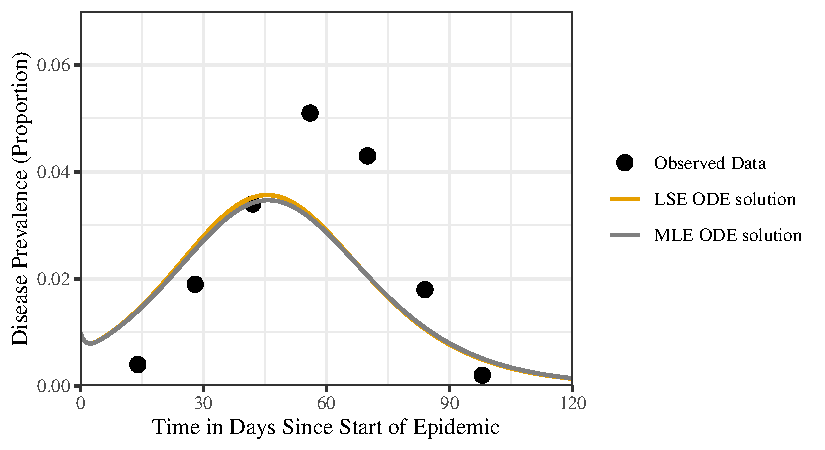
\includegraphics{MLE_SSE_SEIR.pdf}
    \caption{
        An $SEIR$ model fit to some observed prevalence data taken every two
        weeks over a 14 week period, genetated as $I_t/N$ from the $SEIR$
        simulation in Figure \ref{fig:doob_outputs}.
        All parameters were considered known except for $\beta$.
        The least squares estimate (LSE) $\beta^\LS = 0.3516$
        for $\beta$
        was found by solving the model ODEs and numerically minimising the
        square differences between observed prevalences and the ODE prevalences
        (as proportions). Similarly the maximum likelihood estimate
        $\hat{\beta} = 0.3493$ for $\beta$
        was found by assuming the prevalence (times 1000) was binomially
        distributed from 1000 samples with the probability of success being
        equal to $\frac{I_t}{N}.$
    }
    \label{fig:MLE_SSE}
\end{figure}

We demonstrate estimation of one unknown parameter $\beta$ from an $SEIR$ model,
using prevalence data in Figure
\ref{fig:MLE_SSE}. Both $\beta^\LS$ and $\hat{\beta}$ are very close, but do
not fit the data well suggesting fitting the ODEs to a stochastic model
simulation may be a poor choice. This is because at the beginning of an
epidemic the behaviour is very stochastic. Therefore trying to fit an ODE model
to it's stochastic analogue is not necessarily a good idea. The ODEs are more
likely to well approximate the stochastic model when the number of people in
each compartment is high.

\section{Bayesian Parameter Estimation}

In frequentist statistical inference, $\btheta$ is considered to be
fixed, with the observed data $\by^\obs$ assumed to be
generated from a distribution depending on $\btheta.$ Although it is possible
to quantify the uncertainty in parameter estimates through confidence intervals,
frequentist estimates naturally lend themselves to point estimates.
In contrast, inference under a Bayesian
framework assumes that $\btheta$ is also a random variable according to some
pre-known prior distribution. `Evidence' from the observed data then updates
belief about
$\btheta,$ resulting in a posterior distribution of $\btheta,$ described by
Bayes' theorem, namely
$$
    \Pr(\btheta|\by^\obs) \propto \Pr(\by^\obs|\btheta)\Pr(\btheta).
$$

Bayesian parameter estimation is still dependent on the likelihood function
$\mathcal{L}(\btheta) := \Pr(\by^\obs|\btheta).$
With samples from the posterior distribution, we are
able to run our models to capture uncertainty in predicting future scenarios.
For instance, a government may be interested in the number of additional
hospital beds that need to be available to cope with an outbreak of a disease.
If a disease model can be used to approximate outbreaks of the disease,
we can use previous instances of the disease to calibrate our model parameters.
Samples from the posterior parameter distribution, allow
the model to be run multiple times with the varying sets of parameters,
and provide a range of predicted outcomes for the disease. This allows for
confidence in how much investment may be required in the health system.
Similarly, samples from the posterior parameter distribution allow for scenario
modelling such as introducing a new vaccine.

\subsection*{Rejection Sampling}

If we have known ways to sample from the posterior parameter distribution,
then we can use these. However if we have an equation for the probability
distribution, but no way of sampling directly we can sample using rejection
sampling. To sample $X$ through rejection sampling,
we need an explicit way of calculating
$g(x)$ (where $g$ is proportional to the density of $X$), a constant $M$ and
a distribution $p$ such that $Mp(x) \geq g(x)$ with a sampling method
available.

\begin{algorithm}[htbp]
    \caption{Rejection Sampler}
    \label{alg:rej_samp}
    \begin{algorithmic}
        \State Sample $X^\ast \sim p$
        \State Sample $U \sim \mathrm{Unif}(0, 1)$
        \If{$U \leq \frac{g(X^\ast)}{M p(X^\ast)}$}
        \State \Return $X^\ast$ as a sample from the distribution of $X$
        \Else
        \State Repeat
        \EndIf
    \end{algorithmic}
\end{algorithm}

Under this methodology, the distribution function of $X$ is

\begin{align*}
    \Pr(X = x)
    \propto & \Pr(X^\ast = x , U \leq \frac{g(X^\ast)}{M p(X^\ast)})
    \tag*{where the probabilities may be interpreted as densities}                   \\
    =       & \Pr(U \leq \frac{g(X^\ast)}{M p(X^\ast)} | X^\ast = x) \Pr(X^\ast = x) \\
    =       & \frac{g(x)}{M p(x)} p(x)
    =       & \frac{g(x)}{M}
\end{align*}

as required.

\begin{figure}
    \centering
    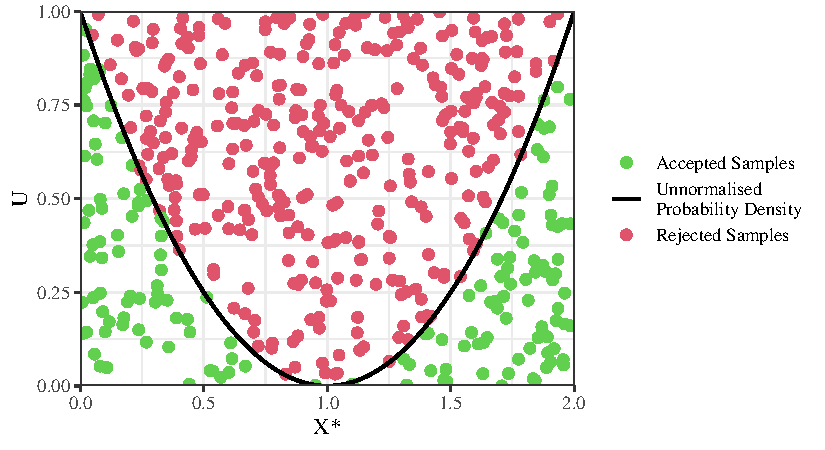
\includegraphics{accept_reject.pdf}
    \caption{
        Samples of $X$ from the unnormalised density $g(x) = (x - 1)^2$ with
        $x\in(0,2)$ using the rejection sampler. $X^\ast\sim\mathrm{Unif}(0,2)$
        and $M = 1.$
        Green dots are samples from
        from $X.$
        Of 500 samples of $X^\ast$, 157 were accepted as samples of $X$.
    }
    \label{fig:accept_reject}
\end{figure}

\begin{example}
    Let $g(x) = (x - 1)^2$ be an unnormalised density function for
    $x \in (0,2).$ $g(x) \leq 1,$ the density of a $\mathrm{Unif}(0,2)$ random
    variable. Therefore to generate samples from $g$ we sample uniformly from
    $X^\ast \sim \mathrm{Unif}(0, 2),$ and then accept the sample if a new
    $U \sim \mathrm{Unif}(0, 1)$ is less than $(X^\ast - 2)^2.$ This is
    demonstrated in \ref{fig:accept_reject}
\end{example}

\subsection*{Markov Chain Monte Carlo Methods}

Often it is not possible to sample directly from the posterior distribution
$\Pr(\btheta|\by^\obs)$ using a rejection sampler, as there is no
explicit form proportional to the true density.
Therefore a common way of sampling from a distribution $p(x)$ is
to construct a Markov chain with stationary distribution $p(x).$
Hence, eventually each new state the
chain moves to will be a be a (not necessarily independent) sample from $p(x),$
or in our case $\Pr(\btheta|\by^\obs).$

\begin{definition}[(Discrete-Time) Markov Chain]
    A sequence of random variables
    $X_0, X_1, \dots$
    is a (discrete-time) \emph{Markov chain} $\{X_i\}_{i\in\mathbb{N}}$ if for
    all
    $k\in\mathbb{N}$,
    $$
        \Pr(X_{i+1}\in A|X_0, X_1, \dots, X_i)
        = \Pr(X_{i+1}\in A|X_i)
    $$
\end{definition}

If $X_i\in\mathcal{X},$ then $\mathcal{X}$ is the state space of the Markov
chain. For example the Markov chain constructed in Figure \ref{fig:MC}, has
discrete state space $\mathcal{X} = \{1, 2\}.$

\begin{figure}[htbp]
    \centering
    \begin{tikzpicture}[>=stealth, auto, semithick]

        % States
        \node[draw, circle] (A) at (0,0) {1};
        \node[draw, circle] (B) at (3,0) {2};

        % Transitions
        \draw[->] (A) to[bend left] node[above] {0.3} (B);
        \draw[->] (B) to[bend left] node[below] {0.4} (A);
        \draw[->] (A) edge[loop above] node {0.7} (A);
        \draw[->] (B) edge[loop above] node {0.6} (B);

    \end{tikzpicture}
    \caption{
        A simple time homogeneous Markov chain, with two states.
        It is characterised by the transition kernel
        $K(1, 1) = \Pr(X_{i + 1} = 1 | X_i = 1) = 0.7,$
        $K(1, 2) = \Pr(X_{i + 1} = 2 | X_i = 1) = 0.3,$
        $K(2, 1) = \Pr(X_{i + 1} = 1 | X_i = 2) = 0.4,$ and
        $K(2, 2) = \Pr(X_{i + 1} = 2 | X_i = 2) = 0.6.$ The stationary
        distribution is $\pi(1) = 4/7$ and $\pi(2) = 3/7.$
    }
    \label{fig:MC}
\end{figure}

Markov chains are characterised by a transition kernel $K$ with
$$K(x_i, x_{i + 1}) := \Pr(X_{i + 1} = x_{i + 1} | X_i = x_{i + 1}),$$
where this probability is interpreted as a density for continuous random
variables. $K(1, 1)$ would therefore be the probability of going from state 1
to state 2.

We will restrict our focus to Markov chains where
if the value of $X_i$ is known to be $x$, behaviour of chain from this point on
will be identical to the behaviour of the chain from $X_j,$ if this is also
observed to be $x$.

\begin{definition}[Time Homogeneous]
    A Markov chain is \emph{time homogeneous} if
    $$
        \{X_i, X_{i+1}, \dots, X_{i + n}\}
        \overset{d}{=} \{X_{i^\prime}, X_{i^\prime+1}, \dots, X_{i^\prime + n}\}
    $$
    for all $i, i^\prime, n \in \mathbb{N},$ given $X_i = x = X_{i^\prime}.$
\end{definition}

The Markov chain in Figure \ref{fig:MC} is time homogeneous. It doesn't
matter how long it took to get into a state, the Markov chain will behave the
same from that point forward.

\begin{definition}[Stationary Distribution]
    A Markov chain has \emph{stationary distribution} $\pi$ if for $X_i \sim \pi,$
    then $X_{i + 1} | X_i \sim \pi.$
\end{definition}

\begin{example}
    Given the Markov chain in Figure \ref{fig:MC}, the stationary distribution
    can be calculated by solving the simultaneous equations
    \begin{align*}
        K(1, 1) \times \pi(1)
        + K(2, 1) \times \pi(2) = 0.7 \times \pi(1)
        + 0.4 \times \pi(2) = & \, \pi(1) \\
        \pi(1) + \pi(2) =     & \, 1.
    \end{align*}
    Therefore $\pi(1) = 4/7$ and $\pi(2) = 3/7.$
\end{example}

As stated earlier, to sample from a distribution $p(x),$ we construct a Markov
chain with this stationary distribution. A sufficient condition to know that
we have achieved this is if our chain satisfies the the detailed balance
condition.

\begin{theorem}[Detailed balance condition]
    A Markov chain has stationary distribution $p(x),$ which it converges to
    independent of initialisation, if for all $x, x^\prime,$
    $$p(x)K(x, x^\prime) = p(x^\prime)K(x^\prime, x).$$
\end{theorem}

\begin{proof}
    More formally this requires the notions of recurrent, nonnull,
    irreducible and aperiodic which we do not discuss here. For a full
    discussion and proof
    see \cite[chapter 6]{robert_monte_2010}.
\end{proof}

\subsubsection*{Metropolis-Hastings}

The Metropolis-Hastings algorithm is one way of constructing a Markov
chain with stationary distribution equal to the target distribution $g.$
We choose a proposal distribution $q(x^\prime| x)$ which given our last sample
$x,$ generates a new random
variable $X^\prime.$ For example $q$ might be the density of
$X^\prime \sim N(x, 1),$ a normal random variable with mean
around the previous sample. Then similar to rejection sampling, then $X^\prime$
is accepted as the next state in the distribution with some probability
$\alpha$, chosen in such a way that if
$X_i \sim g,$ then $X_{i + 1}\sim g.$ Formally this is set out in
Algorithm \ref{alg:MH}.

\begin{algorithm}[htbp]
    \caption{Metropolis-Hastings Sampler}
    \label{alg:MH}
    \begin{algorithmic}
        \State Initialise $x_0$
        \For{$i = 1$ to $N$}
        \State Sample $X^\prime \sim q(x^\prime|x_{i - 1})$
        \State Compute acceptance ratio
        $\alpha
            = \min\left(
            \frac{
            g(x^\prime) q(x_{i - 1}|x^\prime)
            }{
            g(x_{i - 1}) q(x^\prime|x_{i - 1})
            },
            1
            \right)$
        \State Sample $U \sim \text{Uniform}(0, 1)$
        \If{$U \leq \alpha$}
        \State $x_i \gets X^\prime$
        \Else
        \State $x_i \gets x_{i-1}$
        \EndIf
        \EndFor
        \State \Return $\{x_0, x_1, \dots, x_N\}$
    \end{algorithmic}
\end{algorithm}

Note that for symmetric proposal distributions $q(x^\prime|x) = q(x|x^\prime),$
$\alpha$ simplifies to $\min\left(\frac{g(x^\prime)}{g(x)}, 1\right),$ in
which case the algorithm is simply called a Metropolis sampler.

\begin{theorem}
    The chain produced by Algorithm \ref{alg:MH} $\{X_k\}_{k\in \mathbb{N}}$
    has stationary distribution $g$ for proposal distributions that cover the
    support of $g.$
\end{theorem}

\begin{proof}
    We show that the detailed balance condition
    $$
        g(x)q(x^\prime | x)\alpha(x, x^\prime)
        =g(x^\prime)q(x | x^\prime)\alpha(x^\prime, x)
    $$
    where $\alpha(x, x^\prime) = \min\left(
        \frac{
                g(x^\prime) q(x|x^\prime)
            }{
                g(x) q(x^\prime|x)
            },
        1
        \right)$
    is satisfied. Without loss of generality let
    $g(x^\prime) q(x|x^\prime) < g(x) q(x^\prime|x),$ so
    $\alpha(x, x^\prime) = \frac{
            g(x^\prime) q(x|x^\prime)
        }{
            g(x) q(x^\prime|x)
        },$ and $\alpha(x^\prime, x) = 1.$
    \begin{align*}
        g(x)q(x^\prime | x)\alpha(x, x^\prime)
        = & g(x)q(x^\prime | x) \times \frac{
            g(x^\prime) q(x|x^\prime)
        }{
            g(x) q(x^\prime|x)
        }                                                \\
        = & g(x^\prime) q(x|x^\prime)                    \\
        = & g(x^\prime) q(x|x^\prime)\alpha(x^\prime, x)
    \end{align*}
\end{proof}

\begin{figure}[htbp]
    \centering
    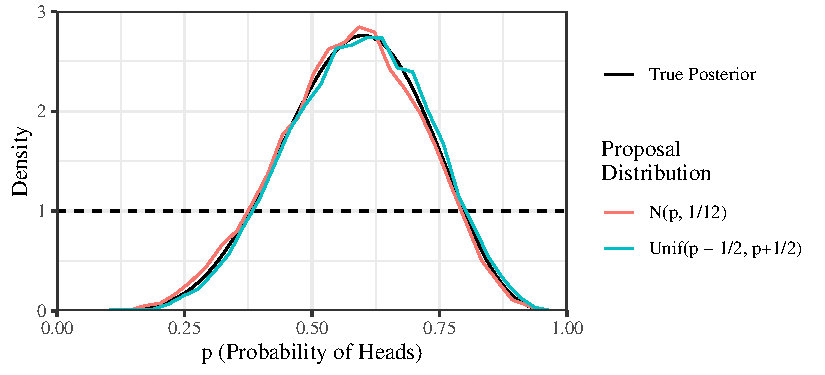
\includegraphics{coin_MH_R.pdf}
    \caption{
        Samples from the posterior distribution of $p$ using the
        Metropolis-Hastings algorithm. $p$ was assumed to
        have a uniform prior between 0 and 1, with $y^\obs = 6,$ generated
        from $\mathrm{Binom}(10, p),$
        The choice of proposal distribution did not impact the final estimate
        of $\Pr(p | y^\obs).$
    }
    \label{fig:coin_R}
\end{figure}

Interestingly, the proof does not depend choice of proposal distribution,
This can be seen in Example \ref{ex:coin_toss} and Figure \ref{fig:coin_R}.

\begin{example}[Coin toss]\label{ex:coin_toss}
    Let the probability of tossing a heads on a weighted coin be
    $\Pr(X = 1) = p.$ Assume that $p\sim \mathrm{Unif}(0,1).$
    We observe $y^\obs = 6$ heads from 10 tosses of the coin.
    Therefore
    $$
        \Pr(p | y^\obs) \propto \Pr(y^\obs| p)\Pr(p)
        = \binom{n}{y^\obs}p^{y^\obs}(1 - p)^{n - y^\obs}\times 1
        = 210p^6(1-p)^4.
    $$
    We sample from this distribution using the Metropolis algorithm which
    becomes
    \begin{algorithmic}
        \State Initialise $p_0$
        \For{$i = 1$ to $N$}
        \State Sample $P^\prime \sim q(p^\prime|p_{i - 1})$
        \State Compute acceptance ratio
        $\alpha
            = \min\left(
            \frac{(P^\prime)^6(1-P^\prime)^4}{p_{i - 1}^6(1-p_{i - 1})^4}, 1
            \right)$ \Comment{Assuming $q$ symmetric}
        \State Sample $U \sim \text{Uniform}(0, 1)$
        \If{$U \leq \alpha$}
        \State $p_i \gets X^\prime$
        \Else
        \State $p_i \gets x_{i - 1}$
        \EndIf
        \EndFor
        \State \Return $\{p_0, p_1, \dots, p_N\}$
    \end{algorithmic}

    We can compare two
    different proposal distributions for $q(p^\prime | p)$,
    $P^\prime \sim N(p, 1/12),$ and
    the second being $P^\prime \sim \mathrm{Unif}(p - 1/2, p + 1/2).$ The first
    1000 samples were discarded as burn in, and it was thinned to every 5
    samples.
    The resulting distribution of the samples can be seen in Figure
    \ref{fig:coin_R}, with both proposal distributions resulting in samples
    that are good at estimating the true distribution.
\end{example}

Since the chain converges to the stationary distribution over time, and is
highly correlated,
a derived chain $\{x_{B + iT}\}_{i \in \mathbb{N}}$ is constructed
from the output. The
first $B$ samples are discarded as `burn in' samples to reduce the impact
of the initialisation point. The chain is `thinned' by taking every $T$th sample,
Since $X_i$ and $X_{i + 1}$ may also be highly correlated (in samples where
the proposed $X^\prime$ is rejected, $X_i = X_{i + 1}$).
This derived chain is considered a
random sample from the target distribution $g.$
In practice, diagnostics such as trace plots and autocorrelation plots are used
to determine $B$ and $T$ are used (see
\cite[chapter 11]{gelman_bayesian_2014}).

\begin{figure}[htbp]
    \centering
    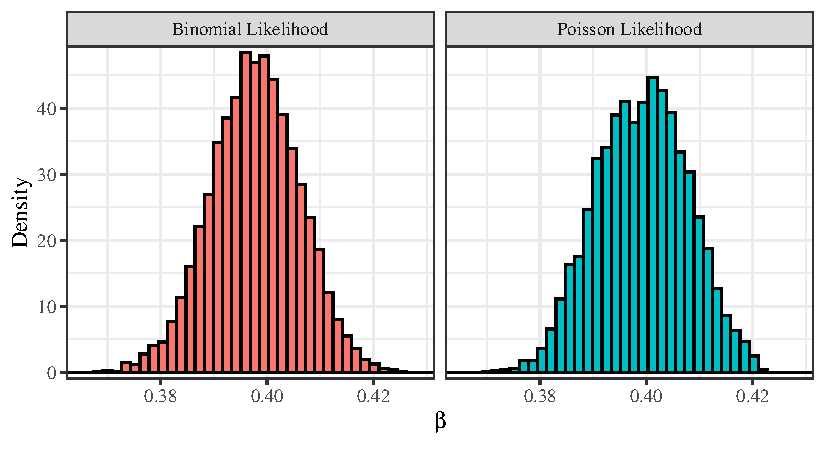
\includegraphics[width=\textwidth]{SIS_beta_pred.pdf}
    \caption{
        Given a daily incidence of $y^\obs = 26$ at day 30 of an $SIS$ epidemic,
        with unknown $\beta,$ we use Metropolis-Hasting to
        sample from $\Pr(\beta | y^\obs).$
        $\gamma = 1/4$ was assumed to be correct, and we compared the assumption
        $y^\obs
            \sim \mathrm{Binom}(\lfloor S_{30} \rfloor,\, \beta I_{30}/N),$
        to the assumption $y^\obs \sim \Pois(\frac{\beta I_{30} S_{30}}{N})$
        where $I_{30}, S_{30}$ are the ODE solutions to Equations
        \ref{eq:SIS_1} and \ref{eq:SIS_2}. We assumed the prior distibution
        $\beta\sim \mathrm{Gamma}(2, 6),$ where $\E(\beta) = 1/3.$ Our proposal
        density was $N(\beta^\ast, 1/10),$ where $\beta^\ast$ was the previous
        sample.
    }
    \label{fig:SIS_MH_R}
\end{figure}

For disease models, given a prior distribution for the parameter(s) $\btheta,$
Metropolis-Hastings can be used to produce samples from
$\Pr(\btheta | y^\obs) \propto \mathcal{L}(\btheta)\Pr(\btheta),$ where
$\mathcal{L}(\btheta)\Pr(\btheta)$ can be calculated to a proportionality
constant but not directly
sampled from. For example given an $SIS$ model with unknown
$\beta \sim \mathrm{Gamma}(2, 6)$ and daily case counts $y^\obs,$ we can
estimate sample from $\btheta | y^\obs$ as in Figure \ref{fig:SIS_MH_R}.

\subsubsection*{Gibbs Sampling}

\begin{algorithm}[htbp]
    \caption{Gibbs Sampler}
    \label{alg:gibbs}
    \begin{algorithmic}
        \State Initialise
        $\btheta^{(0)} = (\theta_1^{(0)}, \theta_2^{(0)}, \dots, \theta_d^{(0)})$
        \For{$i = 1$ to $N$}
        \State Sample
        $\theta_1^{(i)}
            \sim \Pr(
            \theta_1
            | \theta_2^{(i-1)}, \theta_3^{(i-1)}, \dots, \theta_d^{(i-1)}
            )$
        \State Sample
        $\theta_2^{(i)}
            \sim \Pr(
            \theta_2
            | \theta_1^{(i)}, \theta_3^{(i-1)}, \dots, \theta_d^{(i-1)})$
        \State $\vdots$
        \State Sample
        $\theta_d^{(i)}
            \sim \Pr(
            \theta_d
            | \theta_1^{(i)}, \theta_2^{(i)}, \dots, \theta_{d-1}^{(i)})$
        \State Save $(\theta_1^{(i)}, \theta_2^{(i)}, \dots, \theta_d^{(i)})$
        as $\btheta^{(i)}$
        \EndFor
        \State \Return $\{\btheta^{(0)}, \btheta^{(1)}, \dots, \btheta^{(N)}\}$
    \end{algorithmic}
\end{algorithm}

Some models, may have a parameters such that it is possible
to sample from $\theta_1 | \theta_2, \by^\obs$, and
$\theta_2 | \theta_1, \by^\obs$ but not the joint distribution of
$(\theta_1, \theta_2)| \by^\obs.$ A (multidimensional) Markov chain can be
constructed by iteratively updating the parameters. Such a method is called
a Gibbs sampler, described in
Algorithm \ref{alg:gibbs}. The distribution of the Markov chain
sampler will eventually converge to the
$\Pr(\theta_1, \theta_2 | \by^\obs),$ and for the same reasons as for
the Metropolis-Hastings
sampler, after thinning and discarding burn in, we consider the resulting
chain a sequence of independent samples from our target distribution.

\begin{theorem}[Gibbs Sampler]
    The Markov chain generated by Algorithm \ref{alg:gibbs}
    converges to the distribution of $\Pr(\btheta|\by^\obs).$
\end{theorem}

\begin{proof}
    We prove that the Gibbs Sampler satifies the detail balance
    equation for two unknown parameters.
    The transition kernel of the Markov chain is
    $$
        q(\btheta^{(i)}|\btheta^{(i-1)})
        := \Pr(\theta^{(i)}_1 | \theta^{(i-1)}_2, \by)
        \Pr(\theta^{(i)}_2 | \theta^{(i)}_1, \by).
    $$

    To prove the detailed balance condition is satisfied, we need to show that
    $$
        \Pr(\btheta^{(i-1)}| \by)q(\btheta^{(i)}|\btheta^{(i-1)})
        = \Pr(\btheta^{(i)}| \by)q(\btheta^{(i - 1)}|\btheta^{(i)}).
    $$

    \begin{align*}
        \Pr(\btheta^{(t-1)}| \by)q(\btheta^{(i)}|\btheta^{(i-1)})
        = & \, \Pr(\theta_1^{(i-1)}, \theta_2^{(i-1)}| \by) \times
        \Pr(\theta^{(i)}_1 | \theta^{(i-1)}_2, \by) \times
        \Pr(\theta^{(i)}_2 | \theta^{(i)}_1, \by)                        \\
        = & \, \Pr(\theta_1^{(i-1)}| \theta_2^{(i-1)}, \by) \times
        \Pr(\theta_2^{(i-1)}| \by) \times
        \Pr(\theta^{(i)}_1 | \theta^{(i-1)}_2, \by) \times
        \Pr(\theta^{(i)}_2 | \theta^{(i)}_1, \by)                        \\
        = & \, \Pr(\theta_1^{(i-1)}| \theta_2^{(i-1)}, \by) \times
        \Pr(\theta^{(i)}_1, \theta^{(i-1)}_2 | \by) \times
        \Pr(\theta^{(i)}_2 | \theta^{(i)}_1, \by)                        \\
        = & \, \Pr(\theta^{(i)}_2 | \theta^{(i)}_1, \by) \times
        \Pr(\theta^{(i)}_1, \theta^{(i-1)}_2 | \by) \times
        \Pr(\theta_1^{(i-1)}| \theta_2^{(i-1)}, \by)                     \\
        = & \, \Pr(\theta^{(i)}_2 | \theta^{(i)}_1, \by) \times
        \Pr(\theta^{(i)}_1 | \by)  \times
        \Pr(\theta^{(i-1)}_2 | \theta^{(i)}_1, \by) \times
        \Pr(\theta_1^{(i-1)}| \theta_2^{(i-1)}, \by)                     \\
        = & \, \Pr(\theta^{(i)}_1, \theta^{(i)}_2| \by) \times
        \Pr(\theta^{(i-1)}_2 | \theta^{(i)}_1, \by) \times
        \Pr(\theta_1^{(i-1)}| \theta_2^{(i-1)}, \by)                     \\
        = & \, \Pr(\btheta^{(t)}| \by) q(\btheta^{(i -1)}|\btheta^{(i)})
    \end{align*}
    as required, so the posterior pdf $\Pr(\btheta|\by)$ is the unique
    stationary pdf associated with the generated Markov chain.
\end{proof}

\begin{figure}[htbp]
    \centering
    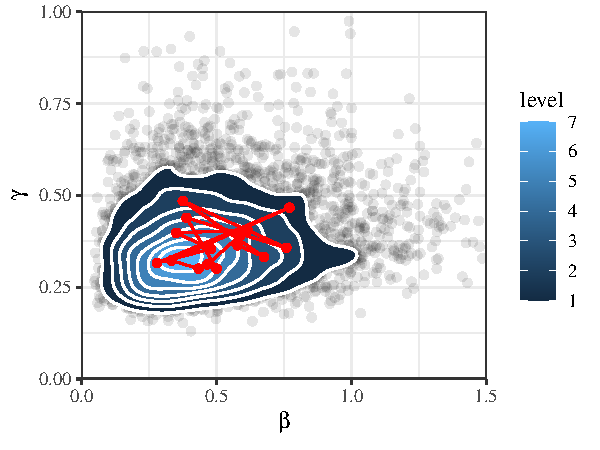
\includegraphics{SIS_gibbs.pdf}
    \caption{
        2000 posterior samples from $\Pr(\beta, \gamma | \by^\obs),$ where
        $\beta|\gamma, \by^\obs
            \sim \mathrm{Gamma}(9, 4/\gamma + 4 + 8\gamma)$ and
        $\gamma|\beta, \by^\obs
            \sim \mathrm{InvGamma}(12, 12\beta).$ The samples were
        obtained using a Gibbs sampler.
        The red points are the first 15 samples using the Gibbs sampler.
    }
    \label{fig:gibbs_R}
\end{figure}

\begin{example}
    Consider the $SIS$ model described by equations \ref{eq:SIS_1}
    and \ref{eq:SIS_2}. Early in an epidemic, the average number of new
    cases generated from a single infectious individual is known as $R_0.$
    This can be shown to be $\frac{\beta}{\gamma}$ for the $SIS$ model.
    Let $\by^\obs = \{1, 1, 3, 1\}$ be the number of people infected by four
    different individuals at the start of the epidemic. We assume that the
    number of infections are generated from a Poisson distribution with mean
    $\frac{\beta}{\gamma}.$ Therefore the likelihood
    $$
        \mathcal{L}(\beta, \gamma):= \Pr(\by^\obs | \beta, \gamma)
        = \frac{
            \left(\frac{\beta}{\gamma}\right)^{1 + 1 + 3 + 1}
            \exp( -\frac{4\beta}{\gamma})
        }{
            1!\times 1! \times 3! \times 1!
        }
        \propto\left(\frac{\beta}{\gamma}\right)^{6}\exp( -\frac{4\beta}{\gamma})
    $$
    Let us assume that from similar previous epidemics we assume that
    $\beta | \gamma \sim \mathrm{Gamma}(3, 4 + 8\gamma),$ and
    $\gamma | \beta \sim \mathrm{InvGamma}(6, 8\beta).$ Therefore
    \begin{align*}
        \Pr(\beta|\gamma, \by^\obs)
        \propto & \Pr(\by^\obs|\gamma, \beta)\Pr(\beta|\gamma)      \\
        \propto &
        \left(\frac{\beta}{\gamma}\right)^{6}
        \exp( -\frac{4\beta}{\gamma})
        \times \beta^{3 - 1}\exp(-(4 + 8\gamma)\beta)               \\
        \propto & \beta^{9 - 1}\exp(-(4/\gamma + 4 + 8\gamma)\beta)
    \end{align*}
    and so
    $\beta|\gamma, \by^\obs
        \sim \mathrm{Gamma}(9, 4/\gamma + 4 + 8\gamma).$
    Similarly
    \begin{align*}
        \Pr(\gamma|\beta, \by^\obs)
        \propto & \Pr(\by^\obs|\gamma, \beta)\Pr(\gamma|\beta)         \\
        \propto &
        \left(\frac{\beta}{\gamma}\right)^{6}
        \exp( -\frac{4\beta}{\gamma})
        \times \gamma^{- 6 - 1}\exp\left(-\frac{8\beta}{\gamma}\right) \\
        \propto & \gamma^{- 12 - 1}
        \exp\left(-\frac{12\beta}{\gamma}\right)
    \end{align*}
    and so
    $\gamma|\beta, \by^\obs
        \sim \mathrm{InvGamma}(12, 12\beta).$
    Now we have explicit forms for the conditional probabilities,
    we generate samples using the Gibbs sampler in Algorithm \ref{alg:gibbs}.
    Samples from the distribution can be seen in Figure \ref{fig:gibbs_R}
\end{example}

The Gibbs sampler and Metropolis-Hastings sampler are often combined, by
using a Metropolis-Hastings sampler for each step of the conditional sampling.
This is useful when the conditional distributions
$\Pr(\theta_1 | \theta_2, \by^\obs)$ can be calculated up to a proportionality
constant, but not directly sampled from.

\subsection*{Approximate Bayesian Computation}

So far, under a Bayesian framework, parameter estimation has still been
dependent on the likelihood function
$\mathcal{L}(\btheta) := \Pr(\by^\obs|\btheta)$ through Bayes' theorem.
In many cases, such as stochastic disease models and agent based models, the
likelihood has no explicit form, or is intractable to calculate.
The only option here is to run the model given $\btheta,$
and sample $\by(\btheta)$ directly.

\begin{algorithm}[htbp]
    \caption{Naive Bayesian Sampler}
    \label{alg:naive_samp}
    \begin{algorithmic}
        \State Sample $\btheta^\ast \sim \Pr(\btheta)$
        \State Run model and compute $\by(\btheta^\ast)$
        \If{$\by(\btheta^\ast) = \by^\obs$}
        \State \Return $\btheta^\ast$ as a sample from $\Pr(\btheta|\by^\obs.)$
        \EndIf
    \end{algorithmic}
\end{algorithm}

A naive method of using such model runs to sample from
$\Pr(\btheta|\by^\obs)$ is to sample
$\btheta^\ast$ from $\Pr(\btheta),$ and run the model to obtain
$\by(\btheta^\ast).$ For each iteration,
$\by(\btheta^\ast)$ will exactly equal $\by^\obs$
with probability $\Pr(\by^\obs|\btheta^\ast)\Pr(\btheta^\ast)
    \propto \Pr(\btheta^\ast|\by^\obs),$
and hence if $\by(\btheta) = \by^\obs$ we can accept $\btheta$ as a sample
from our posterior parameter distribution. This is outlined in
Algorithm \ref{alg:naive_samp}. When
$\by^\obs|\btheta^\ast$ does not have a countable number of non-zero
probability outputs,
$\btheta^\ast = \by^\obs$ can be exactly zero, and even in the
countable case, for
higher dimensional $\by(\btheta),$ the probability of returning exactly
$\by^\obs$ vanishes. Therefore we draw inspiration from the continuous
interpretation of the likelihood
$\mathcal{L}(\btheta) := \Pr(\by(\btheta) \in \diff \by^\obs|\btheta).$
Since

\begin{equation}\label{eq:dens_ball}
    \Pr(\by(\btheta) \in \diff \by^\obs|\btheta)
    := \lim_{\epsilon \to 0}
    \frac{\Pr(\by(\btheta) \in B^D_\epsilon(\by^\obs))}{\varepsilon},
\end{equation}

where $B^D_\epsilon(\by^\obs)$ is a ball of size $\epsilon$ around $\by^\obs,$
with respect to some (unknown) metric $D$ induced by the (unknown)
probability distribution of $\by(\btheta).$ Therefore $\mathcal{L}(\btheta)$ is
approximately proportional
to $\Pr(\by(\btheta) \in B^D_\epsilon(\by^\obs) | \btheta),$
(as a function of $\btheta$).

Hence we construct a new approximate sampling algorithm where rather than
rejecting the sample for $\by(\btheta) \neq \by^\obs,$ we accept
$\by(\btheta)$ if it falls within a ball of size $\epsilon$ around $\by^\obs.$
Equivalently we accept samples if $D(\by(\btheta), \by^\obs) < \epsilon.$

Since the distribution of $\by(\btheta)$ is unknown, and since the metric
required for equation \ref{eq:dens_ball} to hold depends on $\btheta,$ we do
not explicitly derive $D(\by(\btheta), \by^\obs),$ are are forced to
approximate it with $\tilde{D}(\by(\btheta), \by^\obs)$. The most common choice
of $\tilde{D}$ is the $L^p$ norm of $\by(\btheta) - \by^\obs$
$$
    \tilde{D}(\by(\btheta), \by^\obs)
    =||\by(\btheta) - \by^\obs||_p
    = \left(\sum_{i = 1}^d
    \left|y_i(\btheta)
    - y_i^\obs\right|^p\right)^{1/p},
$$
for $p\geq 1.$ For $p=1$ or $2$ this is the Manhattan or Euclidean distance 
between the two vectors. When the observations in $\by^\obs$ are on different
scales, or $\by^\obs$ are highly correlated between model runs, care needs to 
be taken to rescale $\by^\obs$ and $\by(\btheta)$ by a covariance matrix to 
remove correlation, or by rescaling using the relative differences instead of
$||\by(\btheta) - \by^\obs||_p.$

\begin{algorithm}[htbp]
    \caption{Approximate Bayesian Compuation Sampler}
    \label{alg:abc}
    \begin{algorithmic}
        \State Sample $\btheta^\ast \sim \Pr(\btheta)$
        \State Run model and compute $\mathcal{D}(\btheta^\ast)$
        \If{$\mathcal{D}(\btheta^\ast) < \epsilon$}
        \State \Return $\btheta^\ast$ as a sample from $\Pr(\btheta|\by^\obs.)$
        \EndIf
    \end{algorithmic}
\end{algorithm}

Since $\by^\obs$ is fixed, we consider $\tilde{D}(\by(\btheta), \by^\obs)$ as a
function of $\btheta,$ and
we can equivalently write $\mathcal{D}(\btheta) := \tilde{D}(\by(\btheta), \by^\obs).$
We call $\mathcal{D}(\btheta)$ the discrepancy function where in a
non-deterministic model, $\mathcal{D}(\btheta)$ is be random.
. The full procedure is outlined in Algorithm \ref{alg:abc}.
% % \chapter{Bayesian Parameter Estimation}

TODO: \begin{enumerate}
    \item make all single digit numbers words
\end{enumerate}

In classical statistics, $\mathbf\Theta$ is fixed, and the data $Y$ is generated from a distribution depending on $\mathbf\Theta$. Frequentist estimators such as the maximum likelihood estimator, or least squares estimator as previously seen are point estimates. In contrast, inference under a Bayesian framework assumes that $\mathbf\Theta$ is also a random variable. This means although inference may be done on the same model, the Bayesian statistician will more often than not end up with a probability distribution describing $\mathbf\Theta$ given $Y$.

\color{red}
\section{Monte Carlo Integration}

Let us assume we have a random variable $X\sim p,$ and we want to integrate $I = \int_{\mathcal{X}} f(x)p(x)\diff x$ with relation to some known density $p$ and function $f$. We can numerically approximate $I$ by taking $n$ i.i.d. samples $\{x_1, x_2, \dots, x_n\}$ from the distribution specified by $p$, and approximating $I$ by $I_n:=\frac{1}{N}\sum_{i = 1}^nf(x_i).$ By the strong law of large numbers, under specific conditions (for example $\sigma_f := \mathrm{Var}(f(X))<\infty$ is sufficient) we have that $I_n \to I$ almost surely as $n\to\infty$. Furthermore by the central limit theorem we know that $\sqrt{n}(I_n - I) \sim N(0, \sigma_f)$ as $n\to\infty.$ Intuitively, Monte Carlo integration works efficiently because the support set we numerically integrate over are likely to be points of higher probability density that integrating numerically over a set of uniformly distributed points.

\color{black}
\section{Accept-Reject sampling methods}

Accept-Reject methodology fundamentally relies on the theorem that $X\sim f $ is equivalent to simulating $(X,U) \sim \mathrm{Unif}\{(x, u)|0<u<f(x)\}.$ (Theorem 2.15 pg 47 Casella Roberts). In the case where a direct sampling method doesn't exist, we can use this theorem to our advantage. For example, if $a \leq X \leq b$ almost surely, then we can sample the pairs $X^*\sim \mathrm{Unif}(a, b),$ and then $U^*\sim\mathrm{Unif}(0, M),$ where $M\geq \sup_{a<x<b} f(x).$ To then get out samples to follow the distribution of $(X, U)$ we then reject all samples $(x_i, u_i)$ where $u_i>f(x_i).$ The distribution of $X$ can then be described as follows

\begin{align*}
    \Pr(X \leq x) =\, & \Pr(X^* \leq x|U^*\leq f(X^*))                              \\
    =\,               & \frac{\Pr(X^* \leq x, U^*\leq f(X^*))}{\Pr(U^*\leq f(X^*))} \\
    =\,               & \frac{\int_a^xf(y)\diff y/((b - a)*M)}{1/((b - a)*M)}       \\
    =\,               & \int_a^xf(y)\diff y                                         \\
    =\,               & F(x)
\end{align*}

For example in finding samples from the distribution below, we generate 100 random pairs $(X^*, U^*)$

%\begin{tikzpicture}
%\begin{axis}[axis lines = left]
%\addplot[color=red, domain = 0:1]{5*x*(x - 1)^2*(x + 2)};
%% \addplot[blue] coordinates{(\pgfmathparse{rnd}\pgfmathresult, \pgfmathparse{rnd}\pgfmathresult)};
%\end{axis}
%\end{tikzpicture}

%$\foreach \x in {1,...,10}{\pgfmathparse{rnd}\pgfmathresult, }$

There is no need for the distribution to be uniform over the rectangle, and to decrease the number of rejections we can generate points uniformly under a function $h(x)$ that more closely resembles our target distribution as long as $f(x)\leq h(x)$ for all $x$. If $h(x) = Mg(x)$ where $g(x)$ is a probability distribution function with known method of sampling, we can use this to generate via $Y\sim g$ and $U|Y\sim \mathrm{Unif}(0, Mg(x))$ then we reject all pairs where $U|Y>f(Y).$

So in the end we do\texttt{\\
    1. Generate $X\sim g$\\
    2. Accept if $U\leq f(X)/Mg(X)$, otherwise repeat 1.}

If $f$ is computationally expensive, but bounded below by $g_l$, we can \texttt{\\
    1. Generate $X\sim g$\\
    2. Accept if $U\leq g_l(X)/Mg(X)$\\
    3. Accept if $U\leq f(X)/Mg(X)$, otherwise repeat 1.}

\section{Essentials for MCMC}\label{Markov_chains}

\begin{definition}[Random Walk]
    \emph{Random walk} (MCSM 6.1) is a sequence $\{X_n\}$ such that
    $$X_{n+1} = X_n + \varepsilon_n,$$ and $\varepsilon_n$ is independent from $X_1, \dots, X_n$.
\end{definition}

\begin{definition}[Transition Kernel]
    A \emph{transition kernel} is a function $K$ defined on $\mathcal{X}\times\mathcal{B}(\mathcal{X})$ such that\begin{enumerate}
        \item $\forall x\in\mathcal{X},\,\,K(x,\cdot)$ is a probability measure;
        \item $\forall A\in\mathcal{B}(\mathcal{X}),\,\, K(\cdot, A)$ is measureable.
    \end{enumerate} (MCSM 6.2)
\end{definition}

\begin{definition}[Markov Chain]
    Given a transition kernel $K$, a sequence of $X_0, X_1, \dots, X_n, \dots$ of random variables is a \emph{Markov chain} denoted by $(X_n)$ if for any $t$, $$P(X_{k+1}\in A|X_0, X_1, \dots, X_k) = P(X_{k+1}\in A|X_0, \dots, X_k)$$ (MCMS 6.4)
\end{definition}

\begin{definition}[$\varphi$-irreducible]
    Given a measure $\varphi$, the Markov chain $(X_n)$ with transition kernel $K$ is \emph{$\varphi$-irreducible} if, for every $B\in\mathcal{B}(\mathcal{X})$ with $\varphi(A)>0,$ there exists $n$ s.t. $K^n(x, A)>0$ for all $x\in\mathcal{X}$. (MCSM 6.13)
\end{definition}

\begin{definition}[Atom]
    The Markov chain $(X_n)$ has an \emph{atom} ${\alpha\in\mathcal{B}(\mathcal{X})}$ if there exists an associated nonzero measure $\nu$ such that $$K(x, A) = \nu(A)$$ (MCSM 6.18)
\end{definition}

\begin{definition}[Harris Recurrent]
    A set $A$ is \emph{Harris recurrent} if $P_x(\eta_A = \infty) = 1$ for all $x\in A.$ The chain $(X_n)$ is Harris recurrent if there exists a measure $\psi$ such that $(X_n)$ is $\psi$-irreducible and for every set $A$ with $\psi(A) > 0,$ $A$ is Harris recurrent. (MCSM 6.32)
\end{definition}

\begin{definition}[Invariant (Measure)]
    A $\sigma$-finite measure $\pi$ is \emph{invariant} for the transition kernel $K(\cdot,\cdot)$ if $$\pi(B) = \int_\mathcal{X} K(x, B)\pi(\diff x), \forall B\in\mathcal{B}(\mathcal{X})$$ (MCSM 6.35) and $\pi$ is a \emph{stationary distribution} when $\pi$ is a probability measure. If such a $\pi$ exists for a $\psi$-reducible chain, the chain is \emph{positive}.
\end{definition}

\begin{definition}[Ergodic]
    For a positive Harris recurrent chain $(X_n)$, with invariant distribution $\pi$, an atom $\alpha$ is \emph{ergodic} if
    $$\lim_{n\to\infty}|K^n(\alpha, \alpha) - \pi(\alpha)| = 0$$ (MCSM 6.47)
\end{definition}

\color{black}

\section{Motivating the MH/Gibbs Algorithm}
\textcolor{red}{use some of the MC theory to arrive at the acceptance probability in MH}

\section{Metropolis Hastings}

\begin{definition}[Markov Chain Monte Carlo Method]
    A \emph{Markov chain Monte Carlo method} for simulating a distribution $f$ is any method producing an ergodic Markov chain whose stationary distribution is $f$. (MCSM 7.1)
\end{definition}

Given a proposal distribution $q$, and a function $f$ proportional to the posterior distribution, the Metropolis Hastings algorithm is as follows: \texttt{\\
    1. Initialise $X_0$\\
    2. Generate $Y \sim q(y|x)$\\
    3. Calculate $\alpha =
        min\left(\frac{f(y)q(x|y)}{f(x)q(y|x)}, 1\right)$
    4. $X_{t+1} = \begin{cases} Y, & \text{with probability } \alpha\\ X_{t},& \text{else}\end{cases}$
}

If $q$ is symmetric (that is $q(y|x) = q(x|y)$ for all $x, y$), then $\alpha$ simplifies down to $\frac{f(y)}{f(x)},$ and the algorithm is simply called the Metropolis algorithm.

As an example we can consider a series of coin tosses from a weighted coin. Let $p$ be the probability of a head. We assume that $p\sim\mathrm{Unif}(0,1).$ After 10 tosses six heads could be observed. Let $H\sim\mathrm{Binom}(10, p)$ be the number of heads that are tossed.

\begin{align*}
    \Pr(p\in\mathrm{d}p| H= 6)\propto & \, \Pr(H= 6|p\in\mathrm{d}p)\Pr(p\in\mathrm{d}p) \\
    =                                 & \, \binom{10}{6} p^H(1 - p)^{10 - H}             \\
    \propto                           & \, p^6(1 - p)^{4}
\end{align*}

Consider two different (symmetric) proposal distributions $q(p_i|p_{i - 1})$: \begin{itemize}
    \item $p_i^* \sim N(p_{i - 1}, 1/12)$
    \item $p_i^* \sim \mathrm{Unif}(p_{i - 1} - 1/2, p_{i - 1} + 1/2)$.
\end{itemize} Both are symmetric, and so \begin{align*}
    \alpha = & \, \min\left(\frac{f(p_i)q(p_{i - 1}|p_{i})}{f(p_{i - 1})q(p_i|p_{i - 1})}, 1\right)                                         \\
    =        & \, \min\left(\frac{{p_i}^{6}(1 - p_i)^4}{p_{i - 1}^6(1 - p_{i - 1})^4}\mathbb{I}(p_i > 0), 1\right)                          \\
    =        & \, \min\left(\left(\frac{p_i}{p_{i - 1}}\right)^{6}\left(\frac{1 - p_i}{1 - p_{i - 1}}\right)^4\mathbb{I}(p_i > 0), 1\right)
\end{align*} The effect of the choice of proposal distribution is shown in figure \ref{fig:coin_R}.

\begin{figure}[htbp]
    \centering
    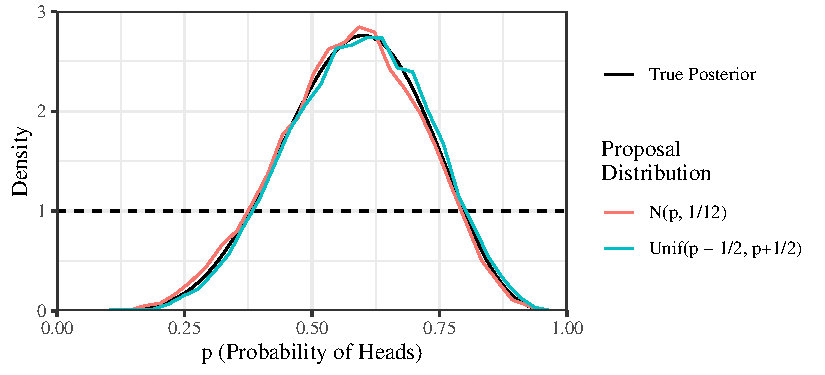
\includegraphics{coin_MH_R.pdf}
    \caption{30,000 samples from the posterior distribution of $p$ using the Metropolis Hastings algorithm. It was assumed that $p\sim \mathrm{U}(0,1)$ and $H \sim \mathrm{Binom}(10, p),$ given $H = 6.$ A uniform and normal proposal distributions were compared.}
    \label{fig:coin_R}
\end{figure}

For another example we can consider a simple SIS epidemiological model, with $$\frac{\diff S}{\diff t} = \gamma I - \beta SI \quad \frac{\diff I}{\diff t} = \beta SI -  \gamma I,$$ and a population of 25,000. Previous pandemics can be used to fix $\beta = 0.5.$ At day 0, it is assumed that there is 1 infected person. Given 1184 new cases on day 30, and $\gamma\sim \mathrm{Gamma}(2, 6)$ we can use the Metropolis Hastings algorithm to sample from the posterior distribution of $\gamma.$  This will depend on the choice of likelihood.\textcolor{red}{Expand this explanation} See figure \ref{fig:SIS_MH_R}

\begin{figure}[htbp]
    \centering
    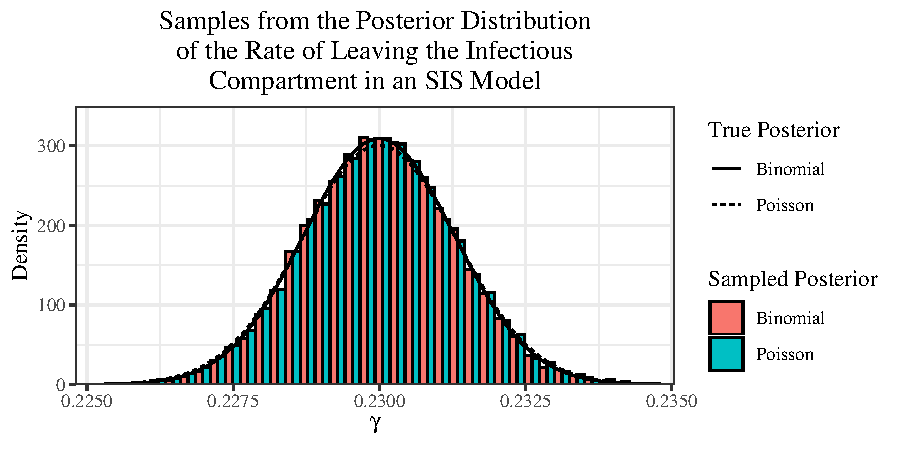
\includegraphics{SIS_gamma_pred.pdf}
    \caption{Using a basic SIS model, using incident changing likelihood function.}
    \label{fig:SIS_MH_R}
\end{figure}

\section{Gibb's Sampling}

For a multivariate case ($\mathbf{\Theta} = \{\theta_1, \theta_2, \dots, \theta_n\}$), it can be analytically or computationally intractable to calculate the posterior (or even something proportional to the posterior) distribution. In this case it may be possible to calculate $\Pr(\theta_i\in\diff\theta|\theta_1, \theta_2, \dots, \theta_{i - 1}, \theta_{i+1}, \theta_{i+2}, \dots, \theta_n, \mathrm{x})$ where $\mathrm{x}$ is the data we are fitting the parameters to.
\textcolor{red}{Prove Gibbs produces sample from the posterior distribution if this is in my final paper}

In this case we can use Gibbs sampling to sample from our posterior distribution. The basic algorithm is as follows:
\texttt{\\
    Initialise for $\mathbf{\Theta} = \{\theta_1, \theta_2, \dots, \theta_n\}$\\
    1. For $i\in\{1, 2, \dots, n\}$ sample $\theta_i^* \sim \theta_i|\theta_1^*, \theta_2^*, \dots, \theta_{i-1}^*, \theta_{i+1}, \dots, \theta_n, \mathbf{x}$\\
    2. Let $\mathbf{\Theta}^* = \{\theta_1^*, \theta_2^*, \dots, \theta_n^*\}$\\
    3. Append $\mathbf{\Theta}^*$ to the chain of parameters, and let $\mathbf{\Theta} := \mathbf{\Theta}^*$
}


\begin{figure}[htbp]
    \centering
    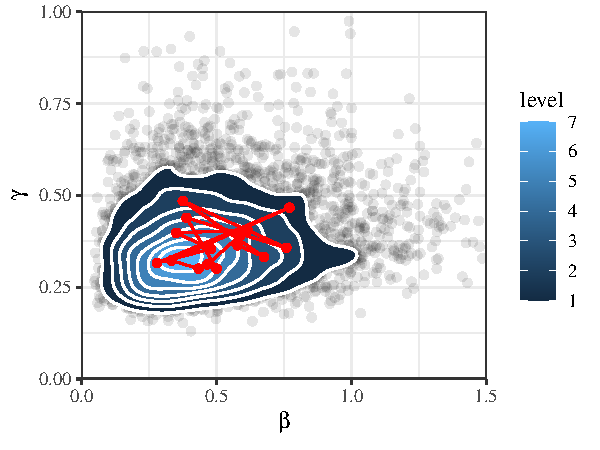
\includegraphics{SIS_gibbs.pdf}
    \caption{Using Gibbs on beta and gamma given an `$R_0$' observation}
    \label{fig:gibbs_R}
\end{figure}

\section{Diagnostics for Metropolis Hastings}
\textcolor{red}{include things like autoregression, thinning, burn-in etc.}
% % \chapter{Approximate Bayesian Computing}

The previous chapter assumes that the likelihood function is known. In reality as models become complicated, the likelihood function often has no closed form or becomes computationally intractable to derive. This is the motivation behind likelihood free techniques.

\section{Exact Likelihood Free Bayesian Computation}

Let $\bm{\theta} = (\theta_i)_{i\in \{1,\dots, n\}}$ be a set of parameters with prior distribution $\pi.$ Given a (random) function $f:$ and $(y_j)_{j\in \{1,\dots, m\}}$ be a set of realised data, generated using $(\theta_i)_{i\in \{1,\dots, n\}}$. The most basic Bayesian computation algorithm is such:
\texttt{\\
    1. Generate $(\hat{\theta_i})_{i\in \{1,\dots, n\}}\sim \pi$\\
    2. Using $(\theta_i)_{i\in \{1,\dots, n\}}$, regenerate the data $(\hat{x_j})_{j\in \{1,\dots, m\}}$ using the\\ parameter set $(\hat{\theta_i})_{i\in \{1,\dots, n\}}$\\
    3. If $(\hat{x_j})_{j\in \{1,\dots, m\}} = (x_j)_{j\in \{1,\dots, m\}}$, accept $(\hat{\theta_i})_{i\in \{1,\dots, n\}}$, else regenerate\\ $(\hat{\theta_i})_{i\in \{1,\dots, n\}}$ and go to step 2
}

For non-discrete cases

Generate parameter(s) from your prior.

Generate the data.

If it matches (or is close enough), add that parameter to your set of accepted parameters. This set will approximate the posterior distribution.

Drawbacks of this approach. Very difficult to estimate multiple parameters to the one outcome parameters. Or if you have a single parameter, generating multiple observations, unlikely to match all of them. Same with multiple parameters to multiple outputs

\begin{figure}[htbp]
    \centering
    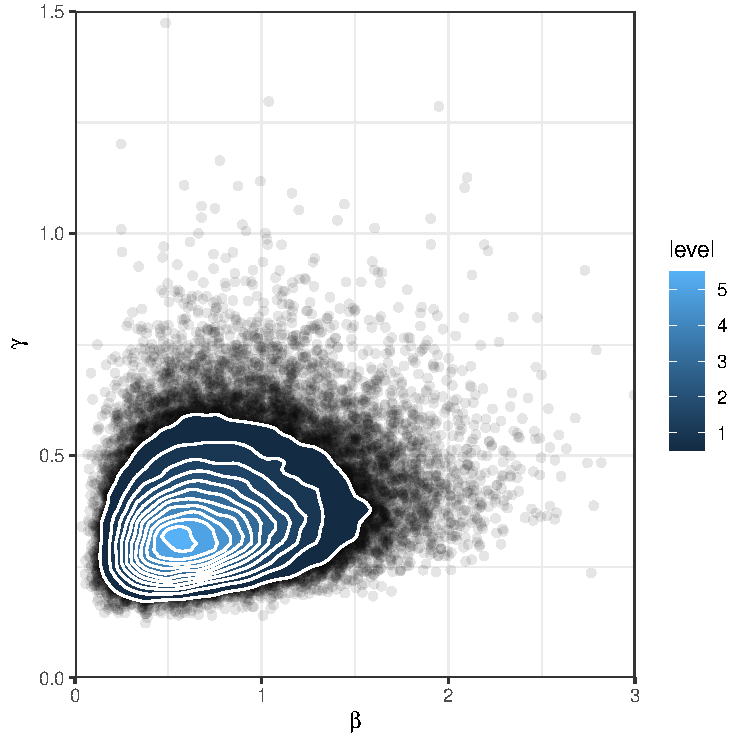
\includegraphics{SIS_ABC.pdf}
    \caption{Using a basic SIS model as in previous figure using ABC to generate from posterior beta, gamma}
    \label{fig:ABC_R}
\end{figure}

\section{Summary Statistics}

\subsection*{Distribution of summary statistic}

Should be relatively normally distributed

\section{Discrepency}

\subsection*{Distribution of discrepency}

|Normal - normal| or something so should be normalish?

\section{Estimating the likelihood from the summary statistic}

See handbook ABC 10 or so
% \chapter{Gaussian Processes}

\begin{itemize}
    \item Prove all pos-sem is cov
    \item expand on intro to motive the section
    \item prove exponential quad kern is pos semi-def
\end{itemize}

\section{Motivation and Preliminaries}

Fundamentally, approximate Bayesian computation is a form of Monte Carlo
integration, where sampling a discrepancy is sampling from the discrepancy
distribution at a given parameter. If we knew the distribution of the
discrepency function exactly, then in order to do approximate
Bayesian computation, we would not need to actually run the model in order to
obtain a `sample' discrepency. Instead we could draw from the distribution of the
discrepency function for a fixed $\bm\theta.$ Further, since acceptance
rejection sampling from our discrepency function approximates something
proportional to the likelihood, if our discrepency function approximation is
close to the actual distribution of the discrepency, we can create an excplicit
synthetic approximate likelihood $\LABC(\bm\theta)\propto \mathcal{L}(\theta)$
and use this directly to obtain posterior samples, or even just find maximimum
likelihood estimates.

To do this, we make the assumptions $\mu(\bm\theta) = \E(D(\bm\theta))$
(or $\E[\ln(D(\bm\theta))] = \mu(\bm\theta)$) is
continuous in theta, $\mathrm{var}(D(\bm\theta)) = \sigma^2$
(or $\mathrm{var}[\ln(D(\bm\theta))] = \sigma^2$) constant for all theta,
and $D(\bm\theta) \sim N(\mu(\bm\theta), \sigma^2)$ for fixed $\bm\theta.$

We consider a class of plausible functions for $\mu(\bm\theta)$, and assign
some underlying prior
probability to each of them. We can then directly simulate from our model to
return a discrepency for a fixed $\bm\theta$ that updates the probability of
each function being the `true' $\mu(\bm\theta)$
function. The class of function we consider are those generated by Gaussian
processes. \textcolor{red}{
    Further discussion on the `distribution' of Gaussian processes on an
    uncountably infinite support is in the appendices.
}

\begin{definition}[Gaussian Process]\label{def:gp}
    A collection of random variables $\{f(x)\}_{x\in\mathcal{X}}$
    (where $x$ may be a vector) is a \emph{Gaussian process} if any finite
    subset of the collection of random variables is multivariate normal
    distributed. That is, there is a function $m:\mathcal{X}\to\R$ and
    symmetric kernel $k:\mathcal{X}\times\mathcal{X}\to \R$ such that for all
    finite sets
    $\mathbf{x} :=\{x_1, x_2, \dots, x_n\} \subset \mathcal{J},$ with
    $f(\mathbf{x}) := [f(x_1), f(x_2), \dots, f(x_n)]^T$
    $$f(\mathbf{x}) \sim
        \MVN\left(\begin{bmatrix}
            m(x_1) \\ m(x_2)\\ \vdots\\ m(x_n)
        \end{bmatrix},\, \mathbf{K} = \begin{bmatrix}
            k(x_1, x_1) & k(x_1, x_2) & \dots  & k(x_1, x_n) \\
            k(x_2, x_1) & \ddots      &        & \vdots      \\
            \vdots      &             & \ddots & \vdots      \\
            k(x_n, x_1) & \cdots      & \cdots & k(x_n, x_n)
        \end{bmatrix}\right).$$
\end{definition}

\begin{definition}[Mean and Covariance Function]\label{def:mean_kernel}
    We define the \emph{mean function} and \emph{covariance kernels} as
    $$m(x_i) := \E\left[f(x_i)\right]$$ and
    $$k(x_{i}, x_{i^\prime}) := \cov\left(f(x_i), f(x_{i^\prime})\right).$$
\end{definition}

For the rest of the discussion, we assume $m \equiv 0,$ but there will be a
brief discussion on non-zero mean functions. Although on $\R^d$ Gaussian
processes are a collection of (uncountably infinite)
random variables, we consider kernels such that
$\mathrm{corr}(x, x^\prime) \to 1$ as $||x - x^\prime||\to 0$ for some norm,
all realisations of the Gaussian process will be continuous in $x$ almost
surely, hence we can consider these as realisations of continuous functions.
\textcolor{red}{(Should I prove this?)}

Some common examples of Gaussian processes include \begin{enumerate}
    \item Brownian motion on $\R$:
          $$m\equiv 0, \quad \text{and}\quad k(s, t) = \min(s, t)$$
    \item Ornstein Uhlenbeck process with parameters $\theta$ and $\sigma$:
          $$
              m\equiv 0, \quad \text{and}
              \quad k(s, t)
              = \frac{\sigma^2}{2\theta} \left(
              e^{-\theta|t - s|} - e^{-\theta(t + s)}
              \right)
          $$
\end{enumerate}

% \begin{definition}[Brownian Motion]
%     $B(t):\R^+ \to \R$ is a \emph{Brownian motion} on $\R$ if\begin{enumerate}
%         \item $B(0) = 0$ almost surely
%         \item $B(t_0), B(t_1) - B(t_0), \dots, B(t_n - t_{n-1})$ are
%               independent for all $t_0<t_1<t_2<\dots<t_n$
%         \item $B(t + s) - B(t)\sim N(0, s)$ for $s, t \geq 0$
%         \item $B(t)$ is continuous almost surely for $t>0.$
%     \end{enumerate}
% \end{definition}

The properties (such as smoothness and rate of fluctuation) of the
realised functions are determined by the class
covariance kernel $k,$ as well as any related hyperparameters. Before exploring
different kernel options, we begin by
\textcolor{red}{defining a valid kernel function, and} formalising `smoothness.'

\color{red}

\begin{definition}[Positive Semi-Definite Matrix]\label{def:pos_def_mat}
    An $n\times n$ matrix $\mathbf{A}$ is \emph{positive semi-definite} if
    $\mathbf{v}^T\mathbf{A}\mathbf{v} \geq 0$ for all $\mathbf{v}\in\R^n.$
\end{definition}

\begin{theorem}[Sufficient Condition for Positive Semi-Definite]
    A symmetric matrix $\mathbf{A}$ is positive semi-definite, if (and only if)
    it's eigenvalues are non-negative.
\end{theorem}
\begin{proof}
    % https://en.wikipedia.org/wiki/Definite_matrix#Eigenvalues
\end{proof}

\begin{definition}[Positive Semi-Definite Kernel]\label{def:pos_def_ker}
    A kernel $k:\mathcal{X}\times\mathcal{X}\to\R$ is
    \emph{positive semi-definite} if the matrix
    $$\mathbf{K} = \begin{bmatrix}
            k(x_1, x_1) & k(x_1, x_2) & \dots  & k(x_1, x_n) \\
            k(x_2, x_1) & \ddots      &        & \vdots      \\
            \vdots      &             & \ddots & \vdots      \\
            k(x_n, x_1) & \cdots      & \cdots & k(x_n, x_n)
        \end{bmatrix}$$
    is positive semi-definite for any collection of $x_i\in\mathcal{X}$
\end{definition}

\begin{theorem}
    All symmetric positive semi-definite matrices are covariance matrices for
    some set of random variables
\end{theorem}
\begin{proof}
    % https://www.fepress.org/wp-content/uploads/2014/06/ch7-iff-covariance_correlation_matrix.pdf
\end{proof}

\color{black}

\begin{definition}[Mean Square Continuous]
    A function $f:\R^d\to\R$ is \emph{mean square continuous} at $\mathbf{x}$
    in the $i$th direction at if
    $\E(|f(\mathbf{x} + h\mathbf{e}_i) - f(\mathbf{x})|^2)\to 0$ as $|h|\to 0,$
    where $\mathbf{e}_i$ is the unit vector with a 1 in the $i$th coordinate.
\end{definition}

\begin{definition}[Mean Square Differentiable]
    A function $f:\R^d\to\R$ is \emph{mean square differentiable} at
    $\mathbf{x}$ in the $i$th direction with derivative
    $\frac{\partial f(\mathbf{x})}{\partial x_i}$ if
    $$
        \E\left[
            \left|
            \frac{f(\mathbf{x} + h\mathbf{e}_i) - f(\mathbf{x})}{h}
            - \frac{\partial f(\mathbf{x})}{\partial x_i}
            \right|^2
            \right]\to 0
    $$ as $|h|\to 0,$ where $\mathbf{e}_i$ is the unit vector in the direction
    of the $i$th coordinate.
\end{definition}

The concept of mean square differentiability and continuity are analogous to
differentiability and continuity in the non-random function case.

\begin{theorem}
    Brownian motion is mean square continuous, but not mean square
    differentiable.
\end{theorem}
\begin{proof}
    $(B_{t + h} - B_t)^2 \sim (\sqrt{|h|}Z)^2$ where $Z\sim N(0,1).$ Therefore
    $(B_{t + h} - B_t)^2 \sim |h|\chi_1^2 \to 0$ almost surely as $|h|\to 0,$
    and hence $\E[(B_{t + h} - B_t)^2= 0]$. Since
    $\frac{B_{t + h} - B_t}{h} \sim N(0, 1/|h|),$ $\frac{B_{t + h} - B_t}{h}$
    does not converge to any valid probability distribution as $|h| \to 0,$ as
    the variance approaches $+\infty.$
\end{proof}

Some common

\color{red}

\begin{theorem}[Positive Semi-Definiteness of RBF]\label{thm:rbf_pos_def}
    The radial basis function
    $\frac{1}{\sigma^2}\exp(-\frac{(x - x^\prime)^2}{2\gamma^2})$ is a positive
    semi-definite kernel.
\end{theorem}

\begin{theorem}[Bochner's Theorem]
    Let $k$ be a stationary kernel function such that
    $k(x, x^\prime) = f(d)$. A function $k:\R^d\to\mathbb{C}$ is the covariance
    function of a weakly
    stationary mean square continuous complex-valued random process of $\R^d$
    if and only if it can be represented as
    $$k(\mathbf{\tau}) = \int_{\R^d} \exp(2\pi i \mathbf{s}\cdot\mathbf{\tau})$$
\end{theorem}

\parencite[82]{rasmussen_gaussian_2008}

\color{black}

\section{Classes of Kernel Function}

\subsection*{Mat\'{e}rn Class}

\begin{figure}
    \missingfigure{Multiple kernels}
\end{figure}

The Mat\'ern class of kernel gives flexibility over how many times mean square
differentiable the realised function is.

The Mat\'ern exponential kernel is of the form
$$k_\nu(x, x^\prime)
    = \sigma^2\frac{2^{1 - \nu}}{\Gamma(\nu)}
    \left(\frac{\sqrt{2\nu}||x - x^\prime||}{\ell}\right)^\nu
    K_\nu\left(-\frac{\sqrt{2\nu}||x - x^\prime||}{\ell}\right)$$
where $K_\nu$ is a modified Bessel function
(see \cite[374]{abramowitz_handbook_2013}). The general form is not very
insightful, but for the most common values of $\nu = 1/2, 3/2$ and $5/2,$ we
have the forms:
$$k_{1/2}(x, x^\prime)
    = \sigma^2\exp\left(-\frac{||x - x^\prime||}{\ell}\right)$$
$$k_{3/2}(x, x^\prime)
    = \sigma^2
    \left(1 + \frac{\sqrt{3}||x - x^\prime||}{\ell}\right)
    \exp\left(-\frac{\sqrt{3}||x - x^\prime||}{\ell}\right)$$
$$k_{5/2}(x, x^\prime)
    = \sigma^2
    \left(
    1 + \frac{\sqrt{5}||x - x^\prime||}{\ell} + \frac{5||x - x^\prime||}{3\ell^2}
    \right)
    \exp\left(-\frac{||x - x^\prime||^2}{2*\ell^2}\right)$$

Zero mean processes with a Mat\'ern kernel are $n$ times mean square
differentiable, for all $n < \nu.$ As $\nu\to\infty,$ with appropriate
rescaling, the limit of the Mat\'ern kernel is the squared exponential
kernel.\cite[85]{rasmussen_gaussian_2008}
\textcolor{red}{LOOK AT CHAPTER 4 SKOROKHOD STOCHASTIC I}

\subsection*{Squared Exponential}

The squared exponential kernel is of the form
$$
    k(x, x^\prime)
    = \sigma^2\exp\left(-\frac{||x - x^\prime||^2}{2\ell^2}\right)
$$

As the limit of Mat\'ern kernels, the squared exponential kernel is infinitely
mean square differentiable. Despite this being the `default' kernel in much of
the literature, infinite differentiability is a very strong condition on
functions.

\subsection*{Choosing an Appropriate Kernel}

The appropriate choice of kernel will depend on the properties behaviour of the
target function to approximate. In the case of estimating an extremely
stochastic distribution (such as the price of a stock over time), it is
unlikely to be smooth, so no mean square differentiability is required, and a
Mat\'ern 1/2 kernel would be appropriate. If it is known that our target
function is extremely smooth, such as a finite sum of infinitely differentiable
functions (such as polynomials, sin, cos etc.) then the choice of squared
exponential kernel is the most appropriate kernel. Realistically, the
smoothness of the function will not be known a priori, and hence some sort of
compromise (such as Mat\'ern 5/2) kernel allows for flexibility.

Many other kernels exist that induce varying behaviours, such as periodic
kernels \textcolor{red}{find periodic kernel}, and non-stationary kernels
(where the covariance is dependent on $x$ and $x^\prime$, not just
$|x - x^\prime|$)
\textcolor{red}{have i defined stationary?}.

\subsection*{Length and Amplitude Hyperparameters}

\begin{figure}
    \missingfigure{different lengths on exponential kernel}
    \caption{a figure about kernel lengths but generated from the same seed}
    \label{fig:no_reg_lengths}
\end{figure}

In both the Mat\'ern and squared quadratic kernels
(as well as most other common kernels), there is a choice of
hyperparameter $\ell,$ called
the length parameter. This value determines how close two points need to be to
be highly correlated. Larger value of $\ell$ generates functions with larger
degrees of local dependence, as seen in Figure \ref{fig:no_reg_lengths}. All kernels
also have an amplitude parameter $\sigma^2.$ The amplitude does not change size
of correlation between $x$ and $x^\prime,$ but just scales the correlation
matrix. In other words, larger $\sigma^2$ increase size but not rate of
fluctuations. This can be seen in Figure \ref{fig:no_reg_amps}.

\begin{figure}
    \missingfigure{GP differing amplitudes}
    \caption{Bunch of GPs generated from the same seed}
    \label{fig:no_reg_amps}
\end{figure}

\section{Gaussian Process Regression}

After choosing a set of prior distributions, given a set of observations, we
can condition our Gaussian process on these priors to update our distribution
of plausible functions. This is where beauty and simplicity in using Gaussian
processes shines through. A conditional multivariate normal distribution
is still multivariate normal, and so the distribution of unobserved points
reduces to elementary linear algebra.

Consider
$$
    \begin{bmatrix}
        f(\mathbf{x}_1) \\
        f(\mathbf{x}_2)
    \end{bmatrix} \sim \mathcal{N}\left(
    \begin{bmatrix}
            m(\mathbf{x}_1) \\
            m(\mathbf{x}_2)
        \end{bmatrix}, \begin{bmatrix}
            K_{11} & K_{12} \\
            K_{21} & K_{22}
        \end{bmatrix}
    \right)
$$


\begin{figure}
    \missingfigure{Progressing GP finding}
\end{figure}




\subsection*{Adding in observation variance}

\begin{figure}
    \missingfigure{GP differing mat\'ern $nu$s}
\end{figure}

New covariance function

\section{Differing mean functions}



\begin{figure}
    \missingfigure{GP mean functions}
\end{figure}


\section{Gaussian Process Regression}

Posterior mean

Posterior variance

\section{Bayesian Acquisition Functions}

\begin{itemize}
    \item Choosing the next point to sample
    \item $\argmin_{\bm{\theta}}A(\bm\theta)$ where A is an acquisition function.
    \item BOLFI paper uses $$\mu(\bm\theta) - \eta_t\sqrt{\mathrm{v}(\bm\theta)}$$ \begin{itemize}
              \item $\eta_t:= \sqrt{c + 2\ln(t^{d/2 + 2})},$ and $c$ can be chosen
              \item $\mu(\bm\theta)$ and $\mathrm{v}(\bm\theta)$ are the posterior mean and variance
          \end{itemize}

    \item Could use expected information
          $$
              (\mu_\text{min} - \mu(\bm\theta)) \varPhi \left(
              \frac{\mu_\text{min} - \mu(\bm\theta)}{\sqrt{\mathrm{v}(\bm\theta)}}
              \right)
              + \sqrt{\mathrm{v}(\bm\theta)}\phi\left(
              \frac{\mu_\text{min} - \mu(\bm\theta)}{\sqrt{\mathrm{v}(\bm\theta)}}
              \right)
          $$
          \begin{itemize}
              \item $\mu_\text{min} := \min_{\bm{\theta}} \mu(\bm\theta)$
              \item $\varPhi, \phi$ CDF and PDF of standard normal
          \end{itemize}
\end{itemize}

exploration parameter proven by \cite{srinivas_gaussian_2010}

% \part{Calibrating Parameters for a \emph{P. vivax} Model}
% \chapter{Methods}

\section{Creation of Synthetic Data}

\begin{figure}[htbp]
    \centering
    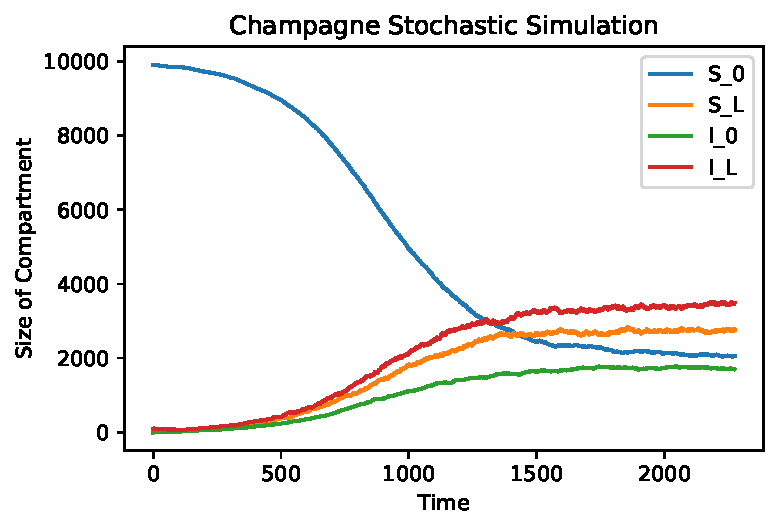
\includegraphics[width = \textwidth]{../champagne_GP_images/champagne_simulation.pdf}
    \caption{
        A Doob-Gillespie Simulation of the model described by
        \cite{champagne_using_2022} with $\alpha = 0.4,$ $\beta = 0.4,$
        $\gamma_L = 1 / 223,$ $\lambda = 0.04,$ $f = 1 / 72,$ $r = 1 / 60,$ and
        $\delta = 0.$ The population was 1000, with 10 initial infections
        (both blood and liver stage).
    }
    \label{fig:champ_doob}
\end{figure}

We investigated the model by \cite{champagne_using_2022} as described in
\ref{sec:champ_mod}. A malaria epidemic was simulated using the Doob-Gillepsie
algorithm (see Figure \ref{fig:champ_doob}), using a population
size of 1,000, and initial infected population of 10 (with both liver and blood
stage infection). The parameters used closely followed those reported in
\cite{champagne_using_2022}: \begin{itemize}
    \item effective blood stage treatment proportion $\alpha = 0.4,$
    \item effective liver stage treatment proportion $\beta = 0.4,$
    \item rate of liver stage disease clearance
          $\gamma_L = 1 / 223 \text{ days}^{-1},$
    \item importation rate $\delta = 0$ (assumed to be known),
    \item rate of infection $\lambda = 0.04 \text{ days}^{-1},$
    \item rate of relapse $f = 1 / 72 \text{ days}^{-1},$
    \item rate of blood stage disease clearance $r = 1 / 60 \text{ days}^{-1}.$
\end{itemize}

From intialisation, the simulation was run for 15,000 events
(with an event being anything that caused the size of any compartment to change
such as an infection, recovery, relapse etc.), after which, the model was
understood to have reached steady state behaviour.

The synthetic data (as summary statistics) measured from the steady state
were:
\begin{enumerate}
    \item $p_\text{obs}:$ the number of currently infected individuals at the
          end of simulated epidemic (steady state prevalence).
    \item $m_\text{obs}:$ the number of cases in the first week of the epidemic
          (first month incidence)
    \item $w_\text{obs}:$ the number of cases in the last week of the epidemic
          (steady state weekly incidence).
\end{enumerate}

New infections which instantly undergo radical cure don't change the size of
each compartment. The number of these `silent' incidences were calculated
between events using a Poisson distribution with rate
$\Delta t \times \alpha \beta \lambda (I_L + I_0) S_0 / N,$ where $\Delta t$ is
the time between events.

\section{Model Simulations and Discrepency Function}

New epidemics were simulated as above, with 15,000 events and at least 30
days (to allow for calculation of incidence in the first month of the
epidemic). For each model run steady state prevalence $p$,
first month incidence $m,$ and steady state weekly incidence $w$ were
calculated with the identical method to the synthetic data.

We defined the discrepency function to be $L_2$ norm of the relative
differences
$$
    \mathcal{D}(\alpha, \beta, \gamma_L, \lambda, f, r)
    := \sqrt{
        \left(\frac{p - p_\text{obs}}{p_\text{obs}}\right)^2
        + \left(\frac{m - m_\text{obs}}{m_\text{obs}}\right)^2
        + \left(\frac{w - w_\text{obs}}{w_\text{obs}}\right)^2
    }.
$$
Relative difference was chosen to limit the impact between the scale
differences of the summary statistics.

\section{Gaussian Process and Initialisation}

We used a Gaussian process $d_\mathcal{GP}(\bm{\theta})$ as a surrogate model for
$\E[\ln\mathcal{D}(\bm{\theta})].$ It was regressed on samples of
$\overline{\ln\mathcal{D}}(\bm{\theta}),$ where
$\overline{\ln\mathcal{D}}(\bm{\theta})$ is the sample mean of 30
$\ln\mathcal{D}(\bm{\theta})$ samples.
We used the kernel
$$
    k(\bm{\theta}_i, \bm{\theta}_i^\prime)
    = \sigma_k^2 (1 + z_i + \frac{z_i^2}{3})\exp(-z_i)
$$
where
$$
    z_i = \sqrt{
        5 \sum_{\theta\in \bm{\theta}}\left(
        \frac{\theta_i - \theta_i^\prime}{\ell_\theta}
        \right)^2
    };
$$ that is, a Mat\'ern kernel with $\nu = 5/2$ and automatic
relevance determination - i.e.\ each parameter $\theta\in\bm{\theta}$ was
scaled by $\ell_\theta.$ This can be seen as giving each parameter its own
length hyperparameter. The Gaussian process was constant mean $m_\mathcal{GP}$
with `observation' variance $\sigma^2_o.$ $\sigma^2_o$ is naturally
intepretable as the sample mean variance.

Modelling the mean of the (log) discrepancy function is theoretically more
sound than modelling the (log) discrepancy function itself, because
we were not able to find theoretically sound reasons to assume normality,
but the mean is asymptotically normal under reasonable conditions by the
central limit theorem. For example, even under the simplest case that the
discrepency is $L_2$ norm of $k$ differences $x_i$ where
$x_i\sim\mathcal{N}(0, 1),$ $\sqrt{\sum_{i=1}^k x_i^2}\sim\chi(k),$ a Chi
distribution with $k$ degrees of freedom.
\textcolor{red}{
    do I need to cite a reference for this distribution (wikipedia)
}

\begin{table}[htbp]
    \centering
    \begin{tabular}{c |c |c}
        Parameter                                                     & Upper Bound & Unit   \\
        \hline
        Proportion of treatment clearing blood stage disease $\alpha$ & 1           &        \\
        Proportion of treatment clearing liver stage disease $\beta$  & 1           &        \\
        Rate of liver stage disease clearance $\gamma_L$              & 1/30        & 1/days \\
        Rate of infection $\lambda$                                   & 1/10        & 1/days \\
        Rate of relapse $f$                                           & 1/14        & 1/days \\
        Rate of blood stage disease clearance $r$                     & 1/14        & 1/days
    \end{tabular}
    \caption{
        Conservative upper bounds for parameters to be calibrated.
        Values were informed by
        \cite{champagne_using_2022, white_variation_2016}. All lower bounds
        were zero.
    }
    \label{table:param_bounds}
\end{table}

All parameters to be calibrated were given conservative upper bounds after
considering values reported in the literature, which informed where to define
the Gaussian process. Parameter values outside this range were not considered.

Latin hypercube sampling was used to generate initialise 50 samples of the
parameter space (scaled to be between zero and the upper bounds described in
Table \ref{table:param_bounds}). For each set of parameters,
$\overline{\ln\mathcal{D}}(\bm{\theta})$ was generated. The hyper\-parameters
$m_\mathcal{GP},$ $\sigma_o^2, \sigma_a^2, \ell_\alpha,
    \ell_\beta, \ell_{\gamma_L}, \ell_\lambda, \ell_f,$
and $\ell_r$ were selected by leave one out cross validation.

\section{Bayesian Acquisition and Parameter Updates}

For 500 iterations, the next $\bm{\theta}$ to sample
$\overline{\ln\mathcal{D}}(\bm{\theta})$ from
at was found by maximising the expected information acquisition function
$\mathcal{A}_\text{EI}(\bm{\theta})$.
Let the current iteration be $t,$ and $d_\mathcal{GP}^{(i)}(\bm{\theta})$
be the Gaussian process regressed on the
simulated $\overline{\ln\mathcal{D}}(\bm{\theta})$s after $i$ iterations.

Each index of $\bm{\theta}$ was initialised randomly at either the
previous sample of $\bm{\theta}$
which minimised $\E(d_\mathcal{GP}^{(t-1)}(\bm{\theta})),$ or uniformly at
random between it's lower and upper bounds. In each iteration, there was a
$\min\left[1/5 + \exp(1 - t/4), 1 \right]$ probability that one of the
parameters (say $\theta^*$) in $\bm{\theta}$
was chosen, and $\overline{\ln\mathcal{D}}(\bm{\theta})$ was sampled at
$\bm{\theta}$ as well as at 11 evenly spaced values of
$\theta^*,$ with the other parameters fixed.
$1/5 + \exp(1 - t/4)>1$ for small $t,$ decaying to $1/5$ as $t$ is
large. This was to help initialise the Gaussian process model, as well as
optimise the $\ell_\theta$s. Every 50 iterations, the hyperparameters were
reoptimised using leave one out cross validation. Finally, the synthetic
likelihood was calculated using
$\hat{\mathcal{L}}(\bm{\theta}) := \Pr(d_\mathcal{N}(\bm{\theta}) < \epsilon),$
where
$d_\mathcal{N}
    \sim \mathcal{N}(\E[d_\mathcal{GP}^{(500)}(\bm{\theta})], 30^2\sigma_o^2)$

The Gaussian process and Gaussian process regression was implemented using
TensorFlow in Python \parencite{abadi_tensorflow_2015}.


% \chapter{Results and Discussion}

\section{Validation}

\begin{table}[htbp]
    \caption{
        Final Gaussian process hyperparameters
    }
    \label{tab:trained_hps}
    \centering
    \begin{tabular}{c|c}
        Hyperparameter    & Final value \\
        $\sigma_o^2$      & $0.07$      \\
        $\sigma_k^2$      & $0.707$     \\
        $\ell_\alpha$     & $0.324$     \\
        $\ell_\beta$      & $0.715$     \\
        $\ell_{\gamma_L}$ & $0.010$     \\
        $\ell_\lambda$    & $0.006$     \\
        $\ell_f$          & $0.016$     \\
        $\ell_r$          & $0.016$     \\
        $m_\GP$           & $0.879$
    \end{tabular}
\end{table}

\begin{figure}[htbp]
    \centering
    \begin{minipage}[b]{0.33\textwidth}
        \centering
        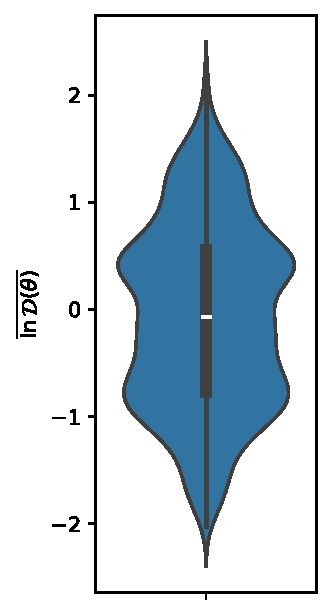
\includegraphics[width=\textwidth]{discreps_violin.pdf}
        \caption{$\smtheta$ violin plot}
        \label{fig:violin}
    \end{minipage}
    \begin{minipage}[b]{0.66\textwidth}
        \centering
        \begin{minipage}[b]{\textwidth}
            \centering
            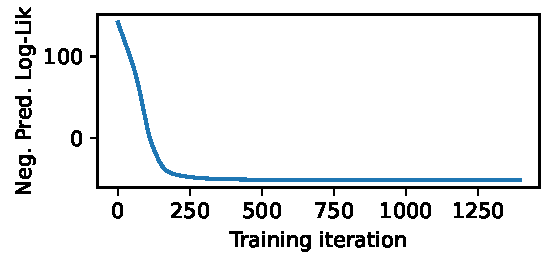
\includegraphics[width=\textwidth]{hyperparam_loss_log_discrep.pdf}
            \caption{Hyperparameter training}
            \label{fig:hyper_train}
        \end{minipage}
        \begin{minipage}[b]{\textwidth}
            \centering
            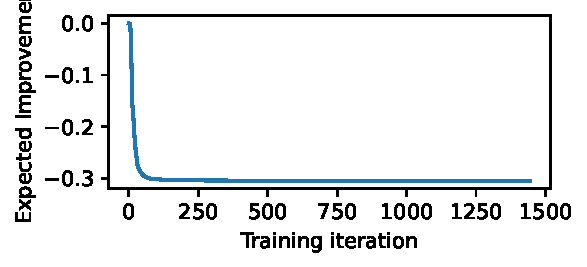
\includegraphics[width=\textwidth]{initial_EI_loss_training.pdf}
            \caption{Finding $\argmin_{\btheta}\A_\EI(\btheta)$}
            \label{fig:subEI}
        \end{minipage}
    \end{minipage}
    % \caption{
    %     Validation of the results from training the Gaussian process. The
    %     \textcolor{red}{something about the discrepancy values being spread}.
    %     }
    % \label{fig:validation}
\end{figure}

The hyperparameters, reported in Table \ref{tab:trained_hps}, and trained
using leave one out cross validation
and expected information acquisition function both
converge smoothly, as seen in Figures \ref{fig:hyper_train} and \ref{fig:subEI},
suggesting the gradient descent algorithm is well optimised.
The violin plot of discrepency function in Figure \ref{fig:violin}
is well dispersed suggesting a good
amount of exploration has been done, but the majority of samples are in the
low discrepency region. This suggests a good exploration exploitation trade-off.

\begin{figure}[htbp]
    \centering
    \begin{subfigure}[b]{0.5\textwidth}
        \centering
        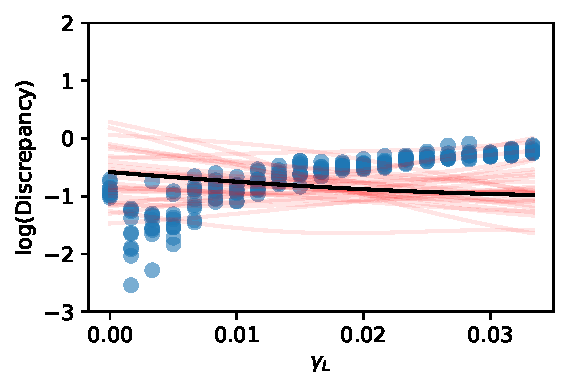
\includegraphics[width=\textwidth]{
            ../champagne_GP_images/initial_gamma_L_slice_log_discrep.pdf
        }
    \end{subfigure}%
    \hfill%
    \begin{subfigure}[b]{0.5\textwidth}
        \centering
        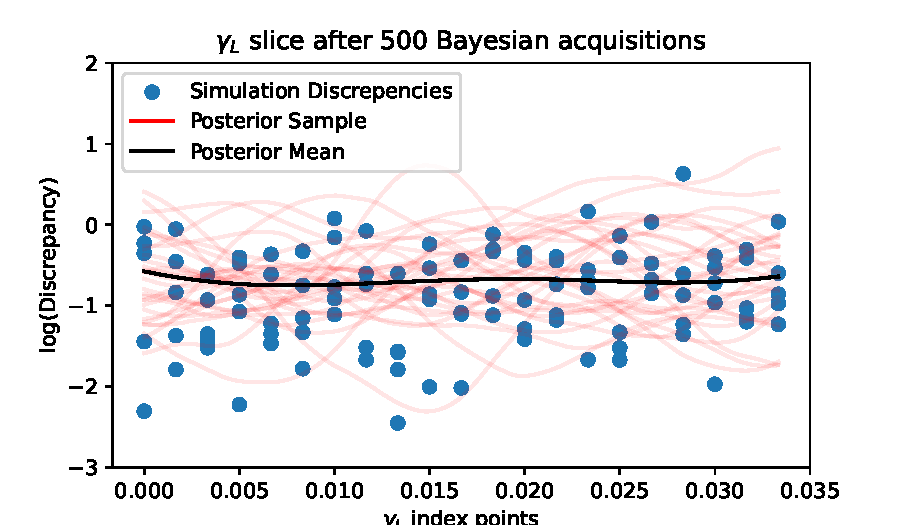
\includegraphics[width=\textwidth]{
            ../champagne_GP_images/gamma_L_slice_500_bolfi_updates_log_discrep.pdf
        }
    \end{subfigure}
    \hfill%
    \begin{subfigure}[b]{0.5\textwidth}
        \centering
        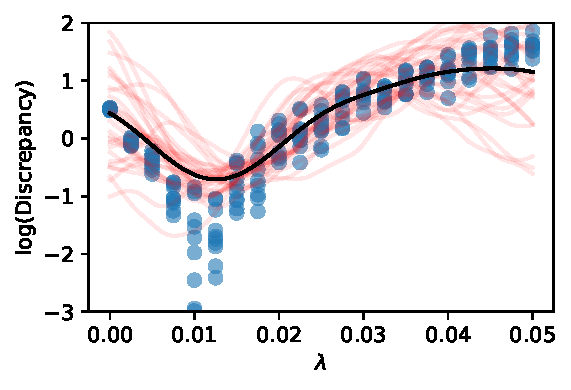
\includegraphics[width=\textwidth]{
            ../champagne_GP_images/initial_lambda_slice_log_discrep.pdf
        }
    \end{subfigure}%
    \hfill%
    \begin{subfigure}[b]{0.5\textwidth}
        \centering
        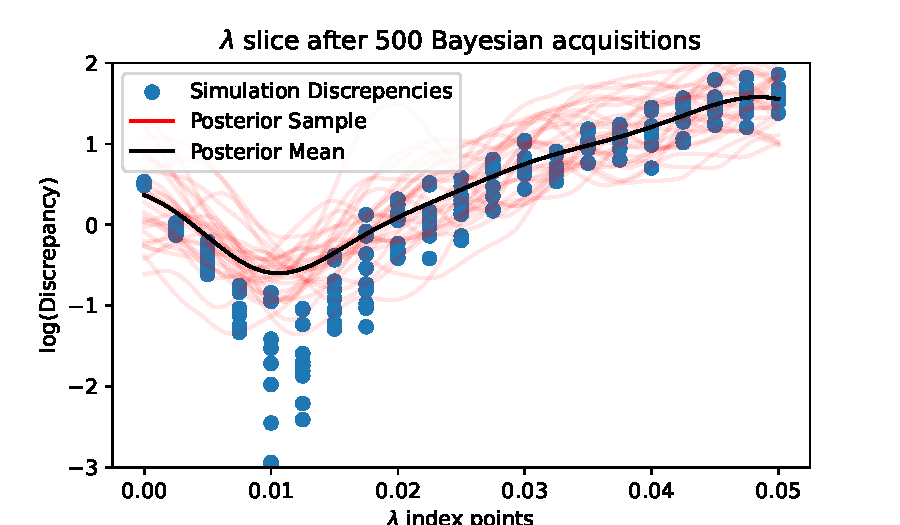
\includegraphics[width=\textwidth]{
            ../champagne_GP_images/lambda_slice_500_bolfi_updates_log_discrep.pdf
        }
    \end{subfigure}
    \begin{subfigure}[b]{0.5\textwidth}
        \centering
        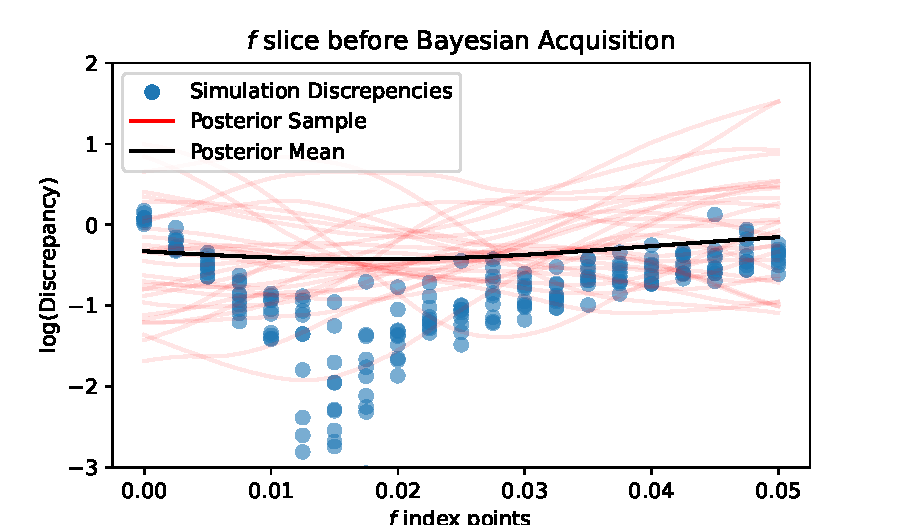
\includegraphics[width=\textwidth]{
            ../champagne_GP_images/initial_f_slice_log_discrep.pdf
        }
    \end{subfigure}%
    \hfill%
    \begin{subfigure}[b]{0.5\textwidth}
        \centering
        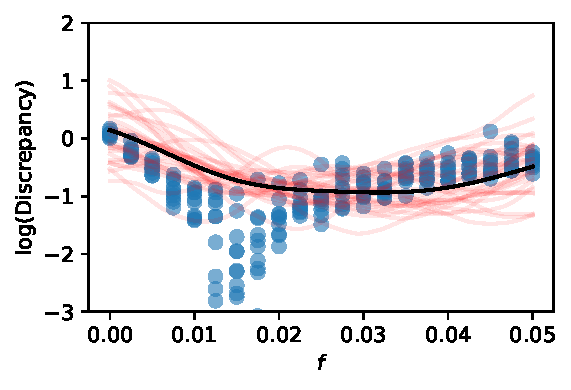
\includegraphics[width=\textwidth]{
            ../champagne_GP_images/f_slice_500_bolfi_updates_log_discrep.pdf
        }
    \end{subfigure}
    \hfill%
    \begin{subfigure}[b]{0.5\textwidth}
        \centering
        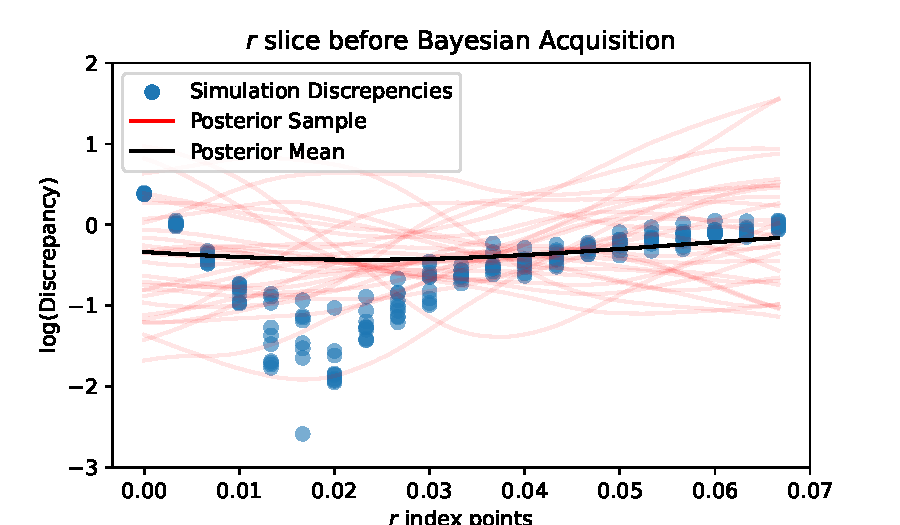
\includegraphics[width=\textwidth]{
            ../champagne_GP_images/initial_r_slice_log_discrep.pdf
        }
    \end{subfigure}%
    \hfill%
    \begin{subfigure}[b]{0.5\textwidth}
        \centering
        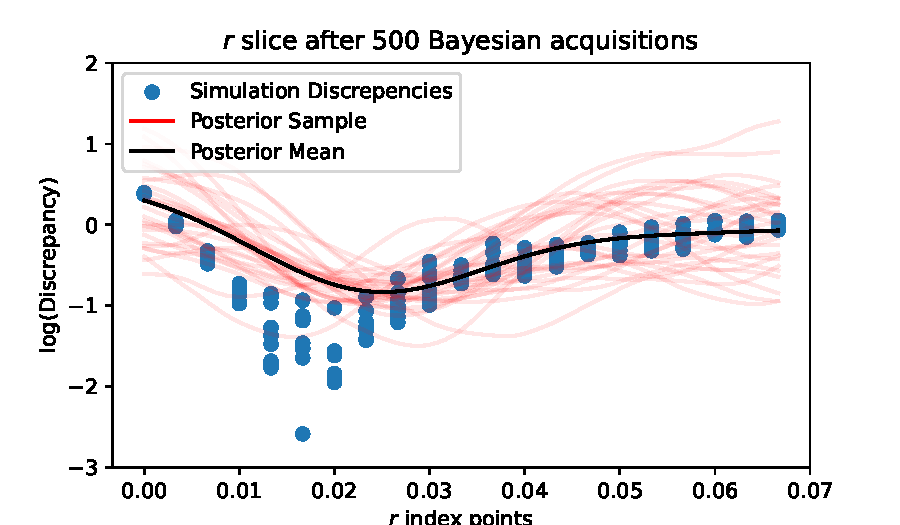
\includegraphics[width=\textwidth]{
            ../champagne_GP_images/r_slice_500_bolfi_updates_log_discrep.pdf
        }
    \end{subfigure}
    \caption{
        The left column of figures is the Gaussian process after initialisation
        $d_\GP^{(0)}(\btheta).$ The black line is $\E(d_\GP^{(0)}(\btheta)),$
        and the red lines are multiple realisations of
        $d_\GP^{(0)}(\btheta).$ The right column of figures is after 500
        sampling iterations, with the black line being
        $\E(d_\GP^{(500)}(\btheta)).$
        The blue dots are realisations of $\ln\mathcal{D}(\bm{\theta}),$ which
        $d_\GP$ approximates predict the mean of. The parameters are varied
        univariately, with all other parameters fixed at the true parameters.
    }
    \label{fig:improving_GP}
\end{figure}

\begin{figure}[htbp]
    \centering
    \begin{subfigure}[b]{0.5\textwidth}
        \centering
        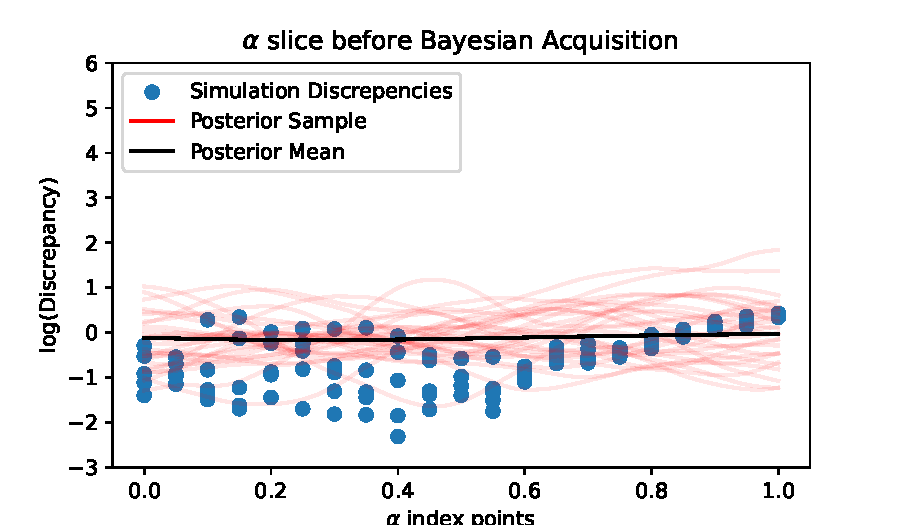
\includegraphics[width=\textwidth]{
            ../champagne_GP_images/initial_alpha_slice_log_discrep.pdf
        }
    \end{subfigure}%
    \hfill%
    \begin{subfigure}[b]{0.5\textwidth}
        \centering
        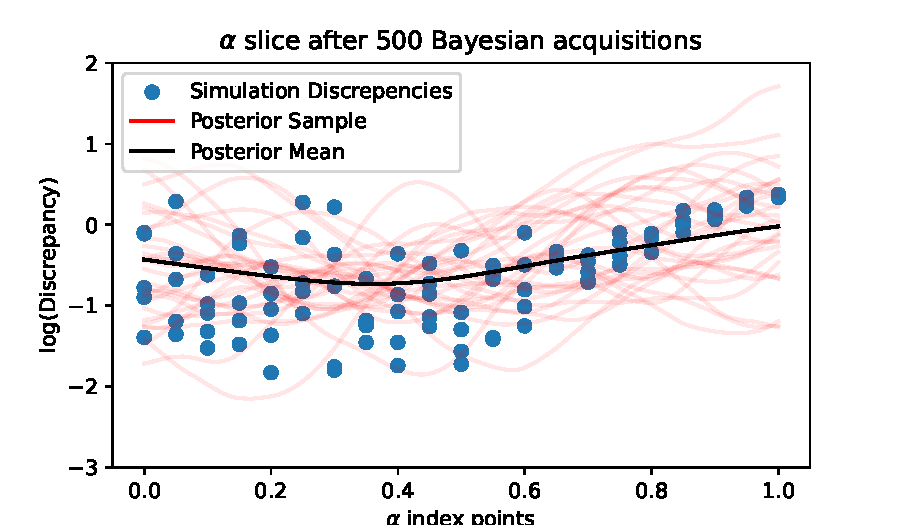
\includegraphics[width=\textwidth]{
            ../champagne_GP_images/alpha_slice_500_bolfi_updates_log_discrep.pdf
        }
    \end{subfigure}
    \hfill%
    \begin{subfigure}[b]{0.5\textwidth}
        \centering
        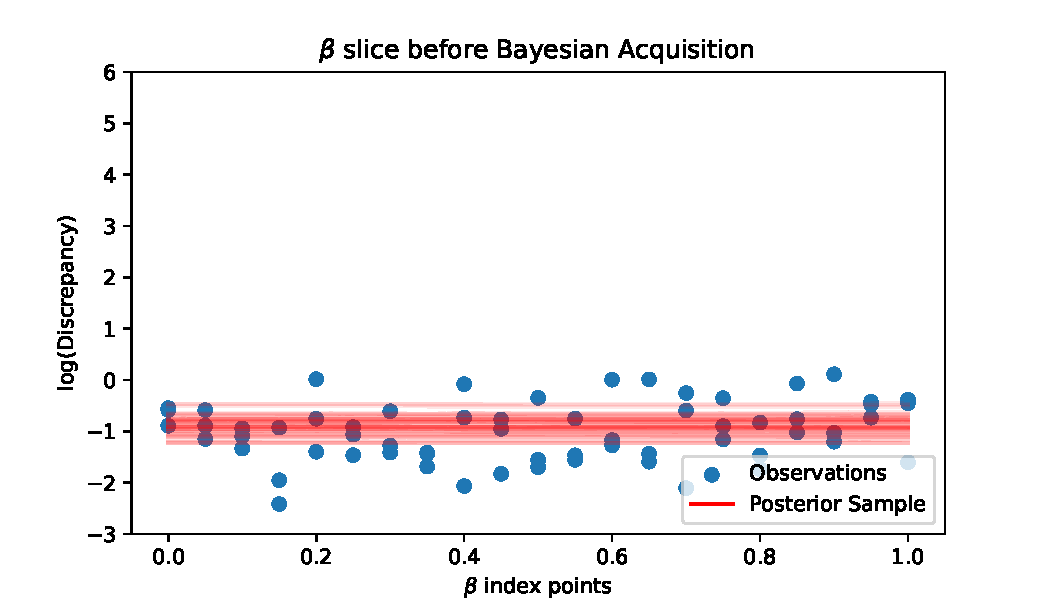
\includegraphics[width=\textwidth]{
            ../champagne_GP_images/initial_beta_slice_log_discrep.pdf
        }
    \end{subfigure}%
    \hfill%
    \begin{subfigure}[b]{0.5\textwidth}
        \centering
        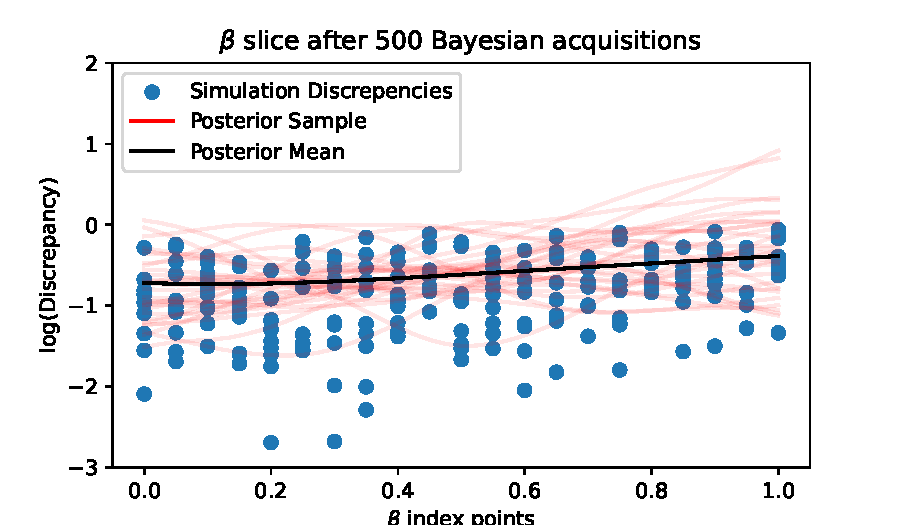
\includegraphics[width=\textwidth]{
            ../champagne_GP_images/beta_slice_500_bolfi_updates_log_discrep.pdf
        }
    \end{subfigure}
    \caption{
        Gaussian process approximations of the treatment parameters, as with
        Figure \ref{fig:improving_GP}
    }
    \label{fig:treatment_GP_fig}
\end{figure}

Figure \ref{fig:improving_GP} suggests that after 500 iterations
$d_\GP(\btheta)$ fits to $\E(\ln\D(\btheta))$ well.
The $\lambda$ slice has the sharpest minimum, whereas $\beta$
does not appear to have much impact on the discrepancy.
As the number of iterations increased, the Gaussian process visibly
improved at fitting to the mean. Interum iterations of $d^{(t)}_\GP(\btheta)$
can be seen in the appendix.

\section{Parameter estimation}

\begin{figure}[htbp]
    \centering
    \begin{subfigure}[b]{0.5\textwidth}
        \centering
        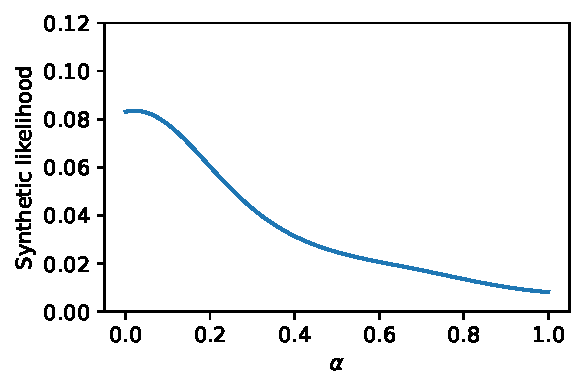
\includegraphics[width=\textwidth]{alpha_slice_synth_likelihood.pdf}
    \end{subfigure}%
    \hfill%
    \begin{subfigure}[b]{0.5\textwidth}
        \centering
        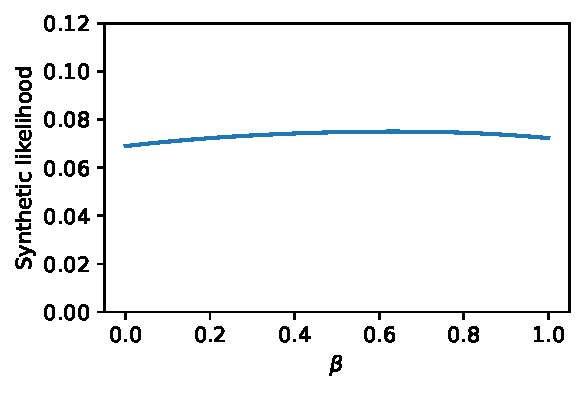
\includegraphics[width=\textwidth]{beta_slice_synth_likelihood.pdf}
    \end{subfigure}
    \begin{subfigure}[b]{0.5\textwidth}
        \centering
        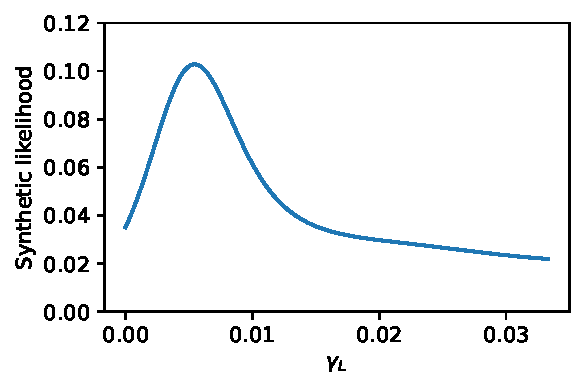
\includegraphics[width=\textwidth]{gamma_L_slice_synth_likelihood.pdf}
    \end{subfigure}%
    \hfill%
    \begin{subfigure}[b]{0.5\textwidth}
        \centering
        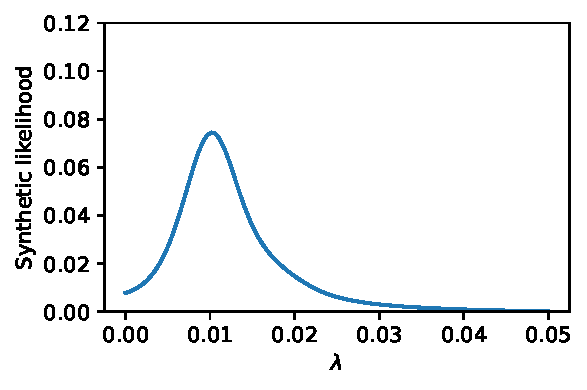
\includegraphics[width=\textwidth]{lambda_slice_synth_likelihood.pdf}
    \end{subfigure}
    \begin{subfigure}[b]{0.5\textwidth}
        \centering
        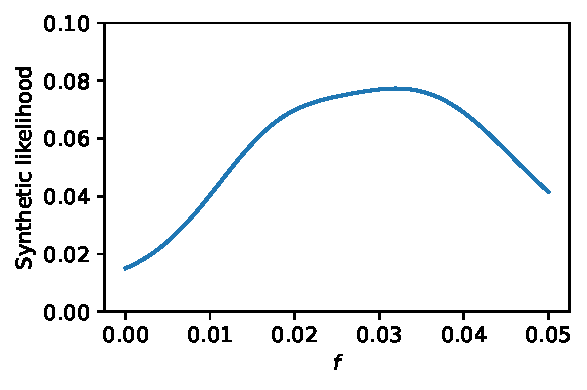
\includegraphics[width=\textwidth]{f_slice_synth_likelihood.pdf}
    \end{subfigure}%
    \hfill%
    \begin{subfigure}[b]{0.5\textwidth}
        \centering
        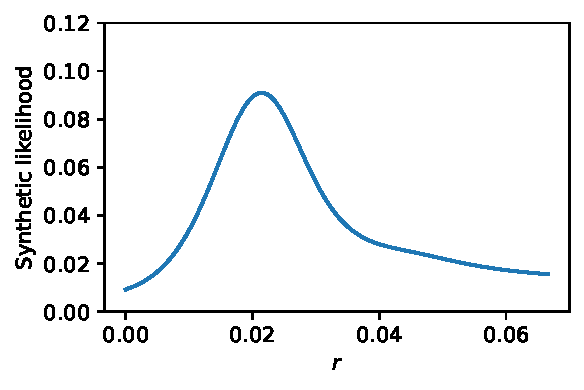
\includegraphics[width=\textwidth]{r_slice_synth_likelihood.pdf}
    \end{subfigure}%
    \caption{
        Final univariate synthetic likelihoods $\hat{L}(\bm{\theta})$ after
        500 sampling iterations. All values not shown were fixed at the true
        parameters.
    }
    \label{fig:final_synth_lik}
\end{figure}

\begin{table}[htbp]
    \caption{
        Estimates of our model parameters.
        The maximum likelihood estimate (MLE) of the true parameters using
        $\hat{L}.$ The maximum slice estimate was the one-dimensional
        maximum likelihood estimate where all other parameters are held
        constant at the true value.
    }
    \label{tab:param_est}
    \centering
    \begin{tabular}{c | c | c | c}
        Parameter  & True     & MLE     & ML Slice Estimate \\
        \hline
        $\alpha$   & $0.124$  & $0.153$ & $0.17$            \\
        $\beta $   & $0.429$  & $0.555$ & $0.52$            \\
        $\gamma_L$ & $0.0026$ & $0.006$ & $0.005$           \\
        $\lambda$  & $0.01$   & $0.01$  & $0.001$           \\
        $f$        & $0.014$  & $0.024$ & $0.02$            \\
        $r$        & $0.017$  & $0.023$ & $0.02$            \\
    \end{tabular}
\end{table}

The synthetic likelihood of each parameter can be seen in Figure
\ref{fig:final_synth_lik}. Unsurprisingly, $\lambda$ has the sharpest peak
in the likelihood function. All likelihoods were unimodal.
The maximum likelihood estimate for $\btheta$ as reported in Table
\ref{tab:param_est} is very close to the true values of the parameters after
500 iterations. This suggests that the synthetic likelihood approximates the
true likelihood well. The maximum likelihood slice estimates were the
univariate maximum likelihood
estimates holding all other parameters at the true value. These are the peaks
in Figure \ref{fig:final_synth_lik}.
Since the maximum likelihood estimate was close to the true parameters,
the maximum likelihood slice estimates were also close to the true values.

\section{Discussion and Future Work}

To our knowledge, the use of the synthetic likelihood as described above
has not been used to calibrate a malaria model before.
\Citeauthor{champagne_using_2022} calibrate the model we use
by find the ODE equilibrium, and fitting a single parameter $\lambda$ to
incidence data. Not only were we able to effectively
recover the true $\lambda$ from a synthetic run, we were able to recover
all model parameters simultaneously.
A similar method has
been set out for infectious diseases in \cite{gutmann_bayesian_2016}.

This methodology is very robust to both frequentist and Bayesian inference.
Under a Bayesian framework,
since we can evaluate the synthetic likelihood for any $\btheta,$
we can use a Metropolis Hasting sampler, to obtain samples from a distribution
approximately equal to the posterior distribution $\Pr(\btheta | \by^\obs).$
Alternatively, standard frequentist inference can also be used on our
synthetic likelihood $\hat{L}.$ For example, numerically approximating the
observed Fisher information matrix
$$
    F(\hat{\theta})
    = -\frac{\partial \ln\hat{L}}{\partial \btheta\partial \btheta^T}(\hat{\btheta})
$$
allows us to do hypothesis testing and construct confidence intervals,
since asymptotically $\hat{\btheta} \sim N(\btheta, F^{-1}(\hat{\btheta}))$
(see \cite{fahrmeir_multivariate_2013}).

Although the likelihood free procedure we outlined for this model closely
resembles \cite{gutmann_bayesian_2016}, there are a few significant changes
that improve on the method outlined in that manuscript.

The most significant change is the choice to model the sample mean as a noisy
Gaussian process, rather than modelling the discrepancy function as a noisy
Gaussian process. Doing this does not lock us in to a distributional assumption
with respect to $\D(\btheta).$ Once we have an approximation for the mean
as a function of $\btheta,$ we could then choose a distribution that scales
with the mean. This is analogous to the generalised linear modelling framework.
For example, it may be reasonable to assume that $\D(\btheta)$ follows a
Gamma distribution. Letting $\mu(\btheta) := \E[\D(\btheta)],$ we can
approximate $\D(\btheta)$ with
$
    \hat{\D}(\btheta)
    \sim \mathrm{Gamma}\left(\frac{\mu(\btheta)}{\phi}, \frac{1}{\phi}\right),
$
where $\frac{\mu(\btheta)}{\phi}, \frac{1}{\phi}$ are the shape and rate
parameters. Trivially
$$
    \E[\hat{\D}(\btheta)]
    = \frac{\mu(\btheta)}{\phi}/\frac{1}{\phi} = \mu(\btheta),
$$
and for a fixed $\phi,$ $\var[\D(\btheta)] = \phi\mu(\btheta),$ so the variance
scales linearly with the mean. If this behaviour is observed
empirically then such a choice will be preferable, since then
$\hat{L}(\btheta)$ will be a better approximation of the the
true likelihood. This can be done with any single parameter distribution with
fixed variance structure.

Alternatively the sample variance could also be modelled with a different
Gaussian process $s^2_\GP(\btheta)$.
Any two parameter distribution could be moment matched by
the two Gaussian processes to get a more accurate $\hat{L}(\btheta).$
Therefore if empirically we observe that $\D(\btheta)$ is approximately Gamma
distributed, then we could approximate $\D(\btheta)$ with
$$
    \hat{\D}(\btheta)
    \sim \mathrm{Gamma}\left(
    \frac{\mu^2(\btheta)}{\sigma^2(\btheta)},
    \frac{\mu(\btheta)}{\sigma^2(\btheta)}
    \right),
$$ where $\var[\hat{\D}(\btheta)] = \sigma^2(\btheta)$ and
$\E(\hat{\D}(\btheta)) =\mu(\btheta)$ as required.

The mean and variance don't have a linked structure in the discrepancy function
which we used for the Champagne model.
This can be seen particularly in the $\lambda$ slice in Figure
\ref{fig:improving_GP}.
For $\btheta$ with $\lambda < 0.03,$ $\var(\ln\D(\btheta))$, is small, and
$\E(\ln\D(\theta))\approx 0$. However for $\lambda \approx 0.02,$ we also have
$\E[\ln\D(\theta)] \approx 0,$ but the variance is observably larger. Therefore
if we had modelled the sample variance of our log discrepency as
as a noisy Gaussian process $s^2_\GP(\btheta)$ then we could have approximated
$\D(\btheta)$ with
$\hat{\D}(\theta) \sim \LN\left(\E(d_\GP(\btheta)), \sigma^2(\btheta)\right),$
where $\mu(\btheta) := \E(d_\GP(\btheta))$ and
$\sigma^2(\btheta) := \E(s^2_\GP(\btheta)).$

Empirically it is not surprising that the variance is not constant across the
parameter space, or even mean dependent. Disease model behaviour is heavily
dependent on the values of the parameters. For example around bifurcation points
a slight change in parameters may lead to a disease model that dies out some
of the time, but reaches equilibrium in other runs. Here we would expect that
$\var[\D(\btheta)]$ to be large. But when $\btheta$ is changed only a small
amount such that the disease consistently dies out, the $\var[\D(\btheta)]$
will be close to $0.$ Since the model
run will always end with a disease free population and the summary statistics
such as incidence or prevalence will always be $0.$ This is likely what is
happen for very small $\lambda$ in Figure \ref{fig:improving_GP}.

This highlights another problem. Around bifurcation points, it is expected that
$\E(\D(\btheta))$ behaves erratically. \cite{gutmann_bayesian_2016} use a
squared exponential kernel for their Gaussian process approximation of
cannot capture this behaviour without
making any length scales very large.
For an example, demonstrating the utility of the Mat\'ern
kernel over the squared exponential in the case of a non smooth function,
see \cite{jones_matern_2021}.
Another possible solution is to use a Student-$t$ process to approximate the
discrepancy, as it has heavier tails, so is more forgiving to sudden jumps.
The multivariate Student-$t$ distribution has some properties analogous to
the multivariate normal distribution. This includes an analytic solution
to the conditional distribution, similar to Theorem \ref{thm:cond_mvn}. For
more details see \cite{shah_studentt_2014}.

\cite{gutmann_bayesian_2016} use the lower confidence bound acquisition
function, where the
exploration parameter is the slowly increasing function
$$\eta_t:= \sqrt{2\ln\left(\frac{t^{2/d + 2}\pi^2}{3\varepsilon}\right)}.$$
This is chosen because under the exponentiated quadratic kernel, and compact
support, the lower confidence bound samples are shown to be no regret with high
probability. There are multiple issues with this. The first is that
\Citeauthor{gutmann_bayesian_2016} seem to have inherited this form from
\cite{brochu_tutorial_2010}. However the citation in
\cite{brochu_tutorial_2010} wrongly reproduces the result in
\cite{srinivas_gaussian_2010},
\footnote{
    One Python package that implements BOLFI notes this error, see:
    \url{
        https://github.com/elfi-dev/elfi/blob/dev/elfi/methods/bo/acquisition.py
    }
} which should be
$$\eta_t:= \sqrt{2\ln\left(\frac{t^{2d + 2}\pi^2}{3\varepsilon}\right)}.$$
When we tried both of these exploration parameters, the choice of
$\varepsilon$ between $(0, 1)$ largely lead to repeated sampling from the same
set of parameters, even for very small $\varepsilon.$ This is similar to the
behaviour reported in \cite{gutmann_bayesian_2016}. Secondly,
\Citeauthor{gelman_bayesian_2014} do not restrict the parameter space to
a compact subset of the space, and so theoretical guarantees of no regret are
not valid. Finally, \Citeauthor{srinivas_gaussian_2010} find this assuming
zero mean Gaussian processes. \Citeauthor{gutmann_bayesian_2016} assume
a quadratic mean prior.

Even though we do consider a compact subset of the parameter space,
we did not use a zero mean Gaussian process, and we used the Mat\'ern kernel,
therefore we did not want to use this formulation of the lower confidence bound,
and instead chose expected improvement.

The quadratic mean assumption in \cite{gutmann_bayesian_2016} is also
problematic. If the mean of the Gaussian process
is trained on a set of data which concave near a local
minimum, no matter which acquisition function is chosen, areas away from the
local minimum may not be sampled from, since the mean function will dominate
the predicted behaviour of $\D(\btheta),$ and so exploration will be minimal.
This also may explain the behaviour of the acquisition function sampling close
to the same point repeatedly.

Although we have validated this method on a relatively low dimensional
$\btheta,$ for models with high dimensionality, it is likely that construction
of a synthetic likelihood will have greater comparitive benefits
to other methods such as approximate Bayesian computation.
This is because as the dimensionality increases, the curse of dimensionality
means that randomly drawn points will be increasingly further away on average,
and so many more samples from the prior distribution function are likely to
produce $\D(\btheta) > \epsilon,$ particularly if $\D(\btheta)$ is small in
a small region. Optimising the acquisition function each time encourages
efficient sampling from areas that are likely to be beneficial to sample from.

One way to reduce the computational overhead of this method would be to reduce
the number of samples were used to calculate the sample mean. This paper used
30 to ensure convergence to the normal distribution, however less could be
taken with the trade off of a larger observation variance. The sample mean
can be calculated in parallel, so the rate limiting step is miminising the
acquisition function each iteration. Rather than sampling
uniformly across a single parameter, multivariate noise could be added to
$\btheta$ to sample multiple sample means at once.
Resources should be maximally allocated
to calculate as many $\D(\btheta)$ as feasible in one step, split between
multiple repeats for the sample mean, and multiple $\btheta$s for better
training of the Gaussian process approximation.
\chapter{Conclusion}

Malaria, a significant global health challenge, continues to burden the 
global health system. Mathematical disease models are increasingly being 
harnessed to alleviate this burden. This thesis explores ways to maximise 
the impact of epidemiological models by ensuring they accurately simulate 
public health scenarios, with a specific focus on the complex issue of 
\textit{P. vivax} malaria. 

The complicated lifecycle of \textit{P. vivax} poses a tough hurdle in 
disease modelling,
particularly with respect to asymptomatic cases and relapses.
This complexity is problematic during the parameter 
calibration stage, where traditional methods that rely on being about to 
compute a likelihood are not viable. Likelihood-free methods, while effective, 
come with a high computational cost due to repeated and inefficient model runs. 
This has led some researchers to calibrate models using deterministic 
approximations, failing to capture the stochastic models' uncertainty. 
There is an obvious need for a better calibration methodology.

This research used Gaussian processes to approximate the distribution of the 
discrepancy function used in approximate Bayesian computation for any set of 
parameters. The true likelihood function was approximated by using the 
Gaussian process to create a synthetic likelihood. Empirical evidence 
demonstrated that this methodology successfully recovered parameters of a 
\textit{P. vivax} model given simulated data while mitigating the 
computational overhead. Additionally, this thesis laid out possible further 
extensions to the methodology.

In conclusion, this thesis has demonstrated the plausibility of a new, 
more robust method of calibrating malaria models, particularly for 
\textit{P. vivax.} The use of Gaussian processes and synthetic likelihoods has 
proven effective in overcoming the infeasibility of traditional calibration 
methods and the computational cost of likelihood-free calibration methods. 
Future research should focus on refining these techniques and exploring their 
application to other infectious diseases. These advancements are crucial for 
developing more effective interventions and ultimately to help support 
achieving malaria eradication.

% %  references and appendix
% \addcontentsline{toc}{part}{Bibliography}
% \printbibliography

% \part{Appendices}

\chapter{Additional Theorems and Proofs}

\begin{theorem}[Sums of Independent Poisson Point Processes]\label{thm:sum_ppp}
    Given independent Poisson point processes $\{\N_1(t)\}_{t\geq0},
        \{\N_2(t)\}_{t\geq0}, \dots,  \{\N_n(t)\}_{t\geq0},$ with intensities
    $\lambda_1, \lambda_2, \dots, \lambda_n,$
    $$\{\N(t)\}_{t\geq0} := \{\N_1(t) + \N_2(t) + \dots + \N_n(t)\}_{t\geq0}$$ is a Poisson point process with intensity $\lambda_1 + \lambda_2 + \dots +
        \lambda_n.$
\end{theorem}

\begin{proof}
    We show that
    $\{\N(t) := \{\N_1(t) + \N_2(t) + \dots + \N_n(t)\}_{t\geq0}\}$ meets each
    component of Definition \ref{def:ppp}.
    \begin{enumerate}
        \item $\N(0) := \N_1(0) + \N_2(0) + \dots + \N_n(0) = 0$ since
              $\N_i(0) = 0$ by definition of a Poisson point process.
        \item We show that $\N(t_1) - \N(t_0), \N(t_2) - \N(t_1), \dots,
                  \N(t_n) - \N(t_{n - 1})$
              with $0 \leq t_0 < t_1 < \dots < t_n$ are independent.
              $$\N(t_i) - \N(t_{i - 1})
                  = \underset{X_{i1}}
                  {\underbrace{[\N_1(t_i) - \N_1(t_{i - 1})]}}
                  + \underset{X_{i2}}
                  {\underbrace{[\N_2(t_i) - \N_2(t_{i - 1})]}} + \dots
                  + \underset{X_{in}}
                  {\underbrace{[\N_n(t_i) - \N_n(t_{i - 1})]}}$$
              $X_{ik}$ is independent of $X_{j\ell}$ for $k \neq \ell$ since
              $\N_k$ and $\N_\ell$ are independent processes. $X_{ik}$ is
              independent of $X_{jk}$ for $i\neq j$ by the second property
              of Definition \ref{def:ppp}. Therefore all $X_{ik}$ are
              independent of $X_{j\ell}$ for $i\neq j,$ and all $j, k.$
              Hence
              $\N(t_1) - \N(t_0), \N(t_2) - \N(t_1), \dots,
                  \N(t_n) - \N(t_{n - 1})$
              with $0 \leq t_0 < t_1 < \dots < t_n$ are independent.
        \item For fixed $t_1 < t_2,$ and $i \in \{1, 2, \dots, n\},$
              $$\N_i(t_2) - \N_i(t_1) \sim \Pois((t_2 - t_1)\lambda_i).$$
              Consider the associated moment generating function of
              $\N_i(t_2) - \N_i(t_1),$
              $$M_i(z) := \exp(\lambda_i(t_2 - t_1)(\exp(z) - 1)).$$
              Therefore the moment generating function of
              $$\N(t_2) - \N(t_1) =
                  [\N_1(t_2) - \N_1(t_1)] + [\N_2(t_2) - \N_2(t_1)] + \dots
                  + [\N_n(t_2) - \N_n(t_1)]$$ is
              $$ M(z) := \prod_{i = 1}^n M_i(z) =
                  \exp[
                      (\lambda_1 (t_2 - t_1) + \lambda_2 (t_2 - t_1) + \dots
                      + \lambda_n (t_2 - t_1))
                      (\exp(z) - 1)
                  ].$$
              Therefore
              $\N_1(t) + \N_2(t) + \dots + \N_n(t) \sim
                  \Pois((\lambda_1 + \lambda_2 + \dots + \lambda_n) t)$
              by the uniqueness of the moment generating function.
    \end{enumerate}
\end{proof}

\begin{theorem}[Time to First Event in Poisson Point Process]
    \label{thm:next_pp_event}
    Given a Poisson point process $\{\N(t)\}_{t\geq 0}$ with intensity
    $\lambda,$ let $\tau = \inf\{t | \N(t_0 + t) - \N(t_0) = 1, t > 0\}$.
    $\tau \sim \Exp(\lambda)$ for $t_0 \geq 0$
\end{theorem}

\begin{proof}
    $$\Pr(\tau > x) = \Pr(\N(t_0 + x) - \N(t_0) = 0)
        = \frac{(\lambda x)^0e^{-\lambda x}}{0!} = e^{-\lambda x}$$
\end{proof}

\begin{theorem}[Probability of $i$th Poisson Process Generating the Next Event]
    \label{thm:which_ppp}
    Consider independent Poisson point processes
    $$\{\N_1(t)\}_{t\geq0},\, \{\N_2(t)\}_{t\geq0},\, \dots,\,
        \{\N_n(t)\}_{t\geq0}$$
    having intensities $\lambda_1, \lambda_2, \dots, \lambda_n.$ For fixed
    $t_0,$ let $\tau_i:=\inf\{t | \N(t_0 + t) - \N(t_0) = 1\}.$
    Then
    $$\Pr(\min_i{\tau_i} = \tau_j)
        = \frac{\lambda_j}{\sum_{i = 1}^n \lambda_i}.$$
\end{theorem}
\begin{proof}
    By Theorem \ref{thm:next_pp_event}, $\tau_i \sim \Exp(\lambda_i).$
    Therefore \begin{align*}
        \Pr(\min_i{\tau_i} = \tau_j) = & \int_0^\infty \Pr(\{\tau_i = x\} \cup \bigcup_{j\neq i}\{\tau_j > x\}) \diff x                    \\
        =                              & \int_0^\infty \Pr(\{\tau_i = x\} \cup \bigcup_{j\neq i}\{\tau_j > x\}) \diff x                    \\
        =                              & \int_0^\infty \Pr(\tau_i = x)\times \prod_{j\neq i}\Pr(\tau_j > x) \diff x\tag{by independence}   \\
        =                              & \int_0^\infty \lambda_i\exp(-\lambda_i x) \times \prod_{j\neq i}\exp(-\lambda_j x) \diff x        \\
        =                              & \lambda_i\int_0^\infty \exp(-(\sum_{i = 1}^n\lambda_j) x) \diff x                                 \\
        =                              & \lambda_i\left[\frac{\exp(-(\sum_{i = 1}^n\lambda_j) x)}{\sum_{i = 1}^n\lambda_j}\right]_0^\infty \\
        =                              & \frac{\lambda_i}{\sum_{i = 1}^n\lambda_j}
    \end{align*}
\end{proof}

\chapter{Additional Results}

\begin{figure}[htbp]
    \centering
    \begin{subfigure}[b]{0.5\textwidth}
        \centering
        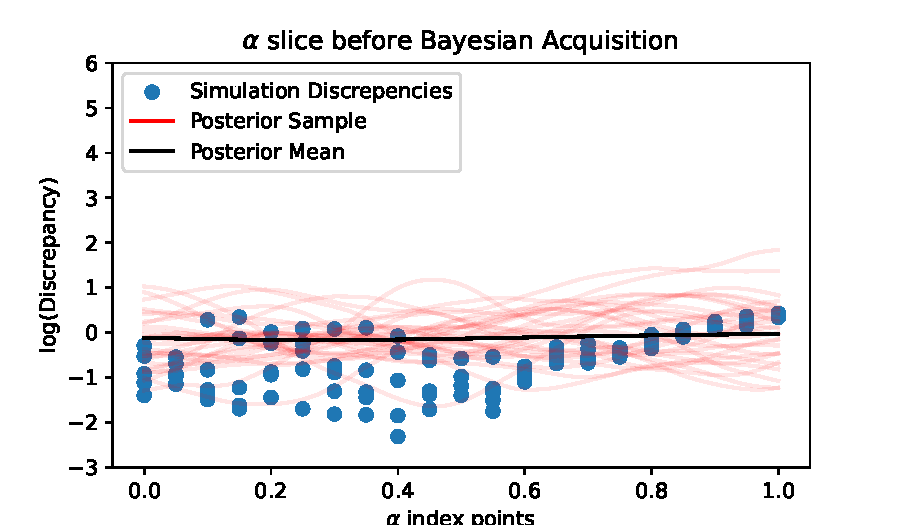
\includegraphics[width=\textwidth]{
            ../champagne_GP_images/initial_alpha_slice_log_discrep.pdf
        }
    \end{subfigure}%
    \hfill%
    \begin{subfigure}[b]{0.5\textwidth}
        \centering
        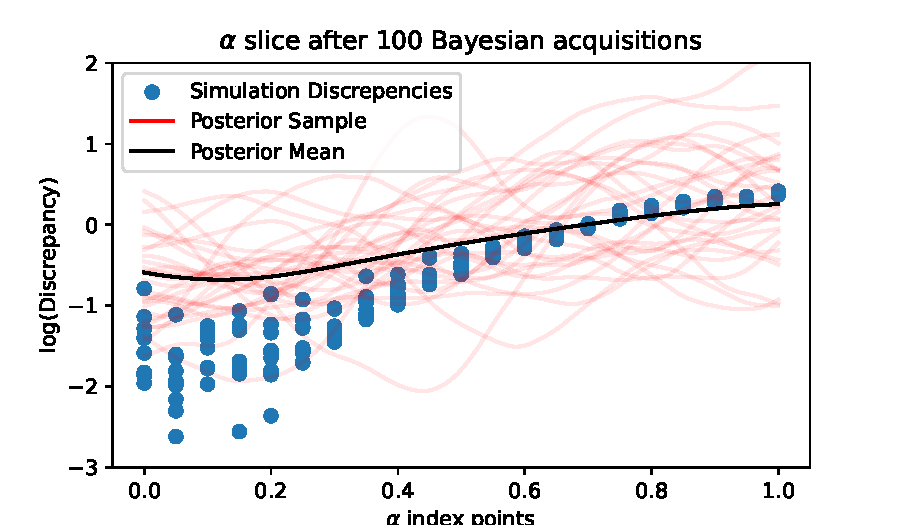
\includegraphics[width=\textwidth]{
            ../champagne_GP_images/alpha_slice_100_bolfi_updates_log_discrep.pdf
        }
    \end{subfigure}
    \hfill%
    \begin{subfigure}[b]{0.5\textwidth}
        \centering
        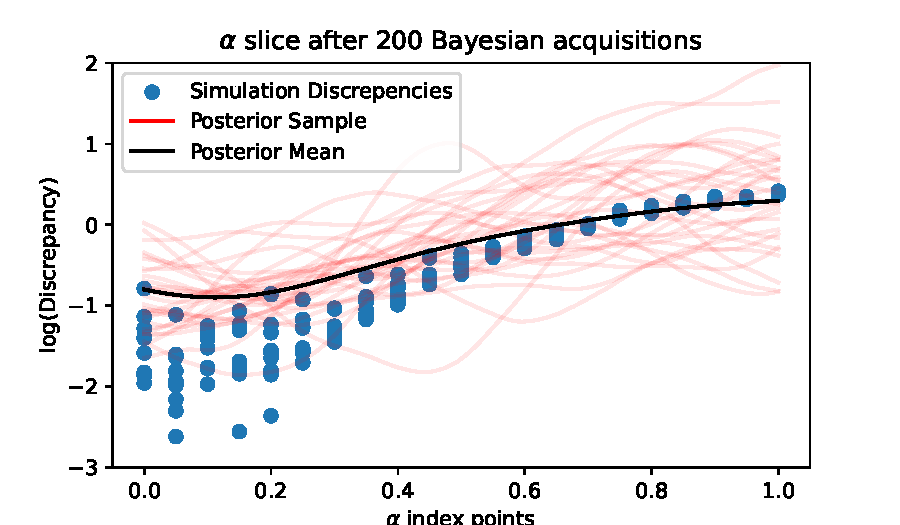
\includegraphics[width=\textwidth]{
            ../champagne_GP_images/alpha_slice_200_bolfi_updates_log_discrep.pdf
        }
    \end{subfigure}%
    \hfill%
    \begin{subfigure}[b]{0.5\textwidth}
        \centering
        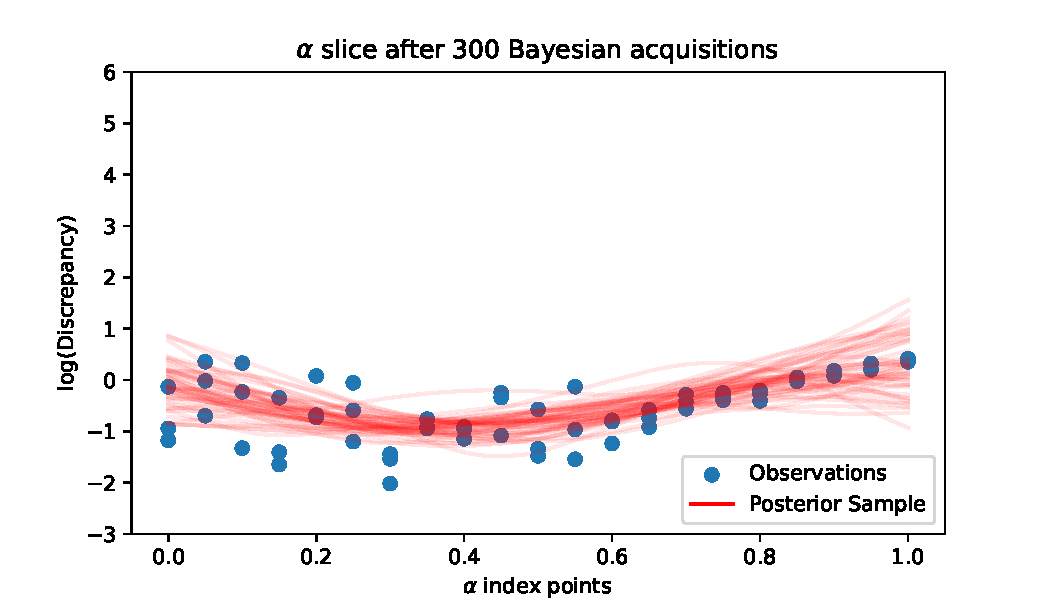
\includegraphics[width=\textwidth]{
            ../champagne_GP_images/alpha_slice_300_bolfi_updates_log_discrep.pdf
        }
    \end{subfigure}%
    \hfill%
    \begin{subfigure}[b]{0.5\textwidth}
        \centering
        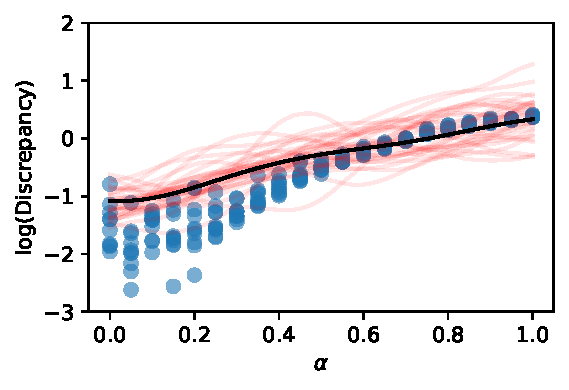
\includegraphics[width=\textwidth]{
            ../champagne_GP_images/alpha_slice_400_bolfi_updates_log_discrep.pdf
        }
    \end{subfigure}
    \caption[{
        Gaussian process regression on $\alpha$ over time
    }]{
        $d_\GP^{(t)}(\btheta)$ approximation of $\E(\ln\D(\btheta)),$ 
        for $t= 0$, $100$, $200$, $300$, and $400.$ Only $\alpha$ was 
        varied. All other parameters were fixed at the true values. Black line 
        is
        $\E(d^{(i)}(\btheta)).$
        Blue dots are realisations from $\ln\D(\btheta).$
    }
\end{figure}

\begin{figure}[htbp]
    \centering
    \begin{subfigure}[b]{0.5\textwidth}
        \centering
        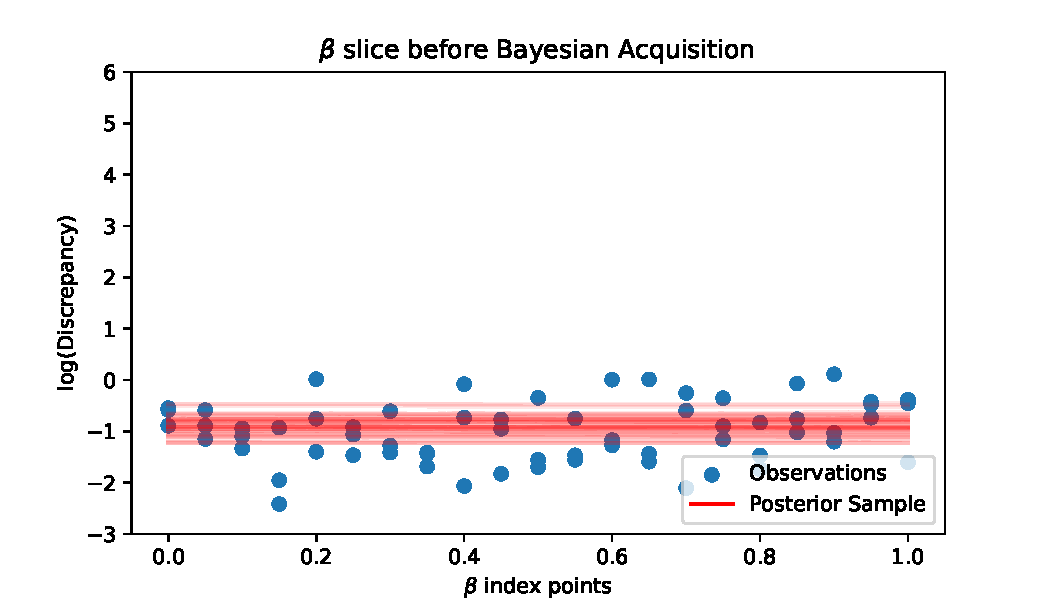
\includegraphics[width=\textwidth]{
            ../champagne_GP_images/initial_beta_slice_log_discrep.pdf
        }
    \end{subfigure}%
    \hfill%
    \begin{subfigure}[b]{0.5\textwidth}
        \centering
        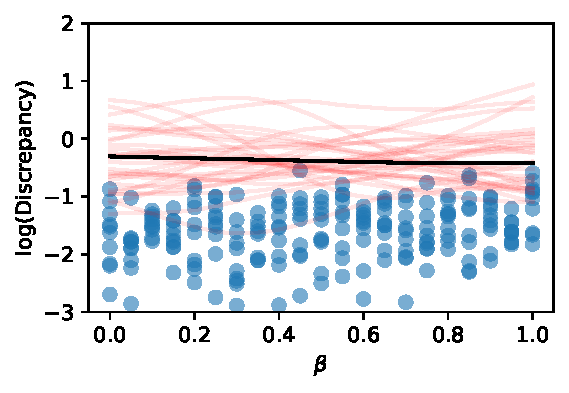
\includegraphics[width=\textwidth]{
            ../champagne_GP_images/beta_slice_100_bolfi_updates_log_discrep.pdf
        }
    \end{subfigure}
    \hfill%
    \begin{subfigure}[b]{0.5\textwidth}
        \centering
        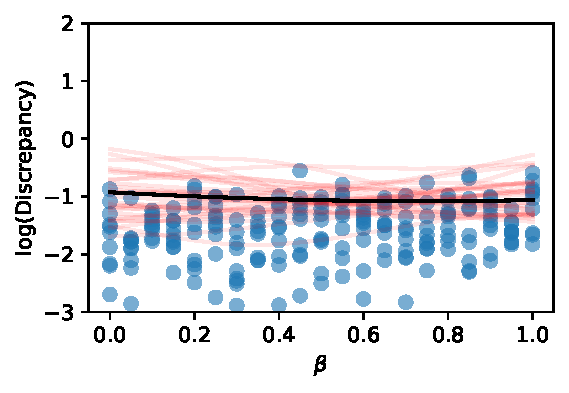
\includegraphics[width=\textwidth]{
            ../champagne_GP_images/beta_slice_200_bolfi_updates_log_discrep.pdf
        }
    \end{subfigure}%
    \hfill%
    \begin{subfigure}[b]{0.5\textwidth}
        \centering
        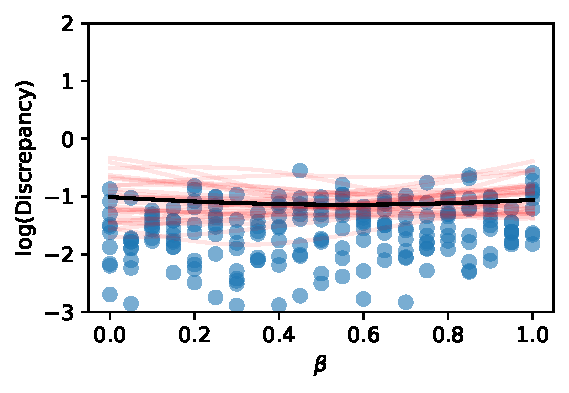
\includegraphics[width=\textwidth]{
            ../champagne_GP_images/beta_slice_300_bolfi_updates_log_discrep.pdf
        }
    \end{subfigure}%
    \hfill%
    \begin{subfigure}[b]{0.5\textwidth}
        \centering
        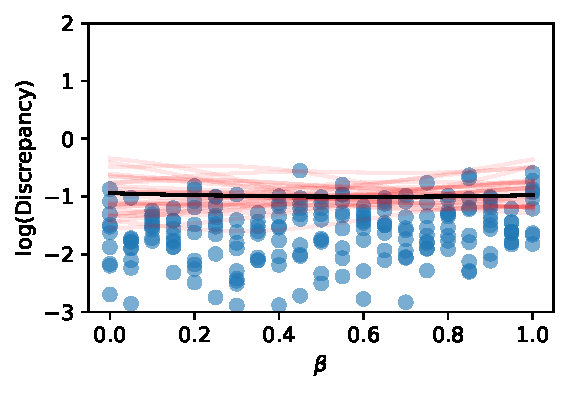
\includegraphics[width=\textwidth]{
            ../champagne_GP_images/beta_slice_400_bolfi_updates_log_discrep.pdf
        }
    \end{subfigure}
    \caption[{
        Gaussian process regression on $\beta$ over time
    }]{
        $d_\GP^{(t)}(\btheta)$ approximation of $\E(\ln\D(\btheta)),$ 
        for $t= 0$, $100$, $200$, $300$, and $400.$ Only $\beta$ was 
        varied. All other parameters were fixed at the true values. Black line 
        is
        $\E(d^{(i)}(\btheta)).$
        Blue dots are realisations from $\ln\D(\btheta).$
    }
\end{figure}

\begin{figure}[htbp]
    \centering
    \begin{subfigure}[b]{0.5\textwidth}
        \centering
        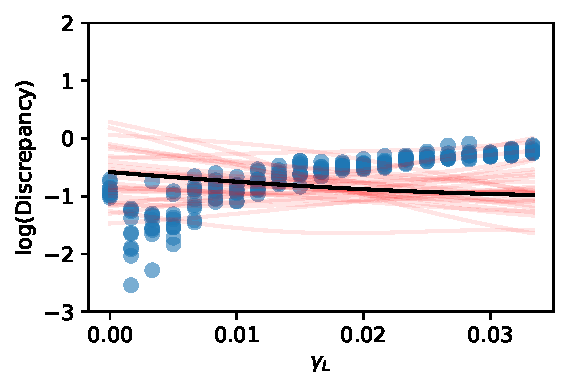
\includegraphics[width=\textwidth]{
            ../champagne_GP_images/initial_gamma_L_slice_log_discrep.pdf
        }
    \end{subfigure}%
    \hfill%
    \begin{subfigure}[b]{0.5\textwidth}
        \centering
        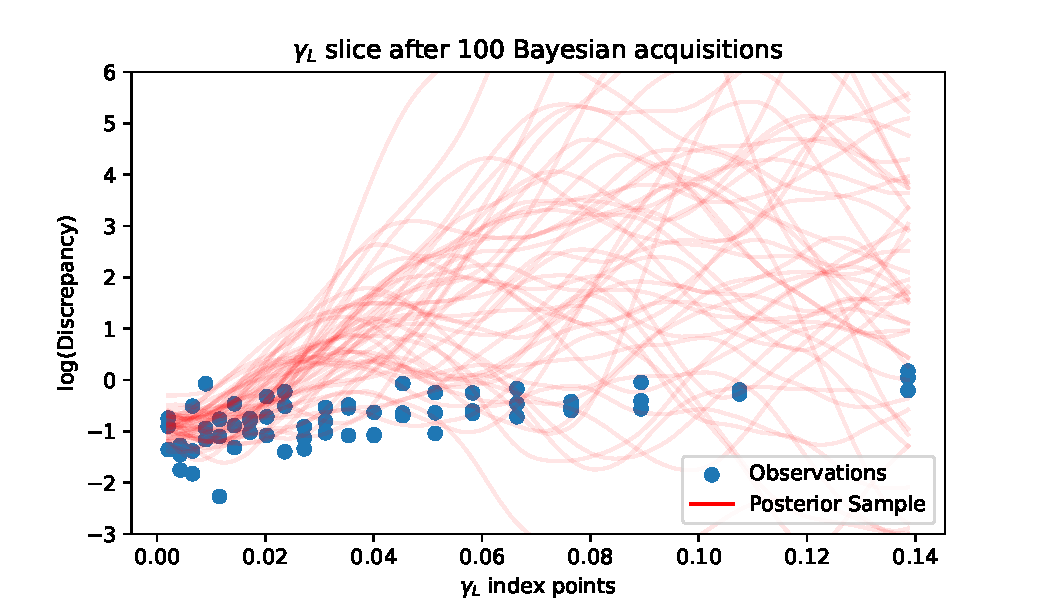
\includegraphics[width=\textwidth]{
            ../champagne_GP_images/gamma_L_slice_100_bolfi_updates_log_discrep.pdf
        }
    \end{subfigure}
    \hfill%
    \begin{subfigure}[b]{0.5\textwidth}
        \centering
        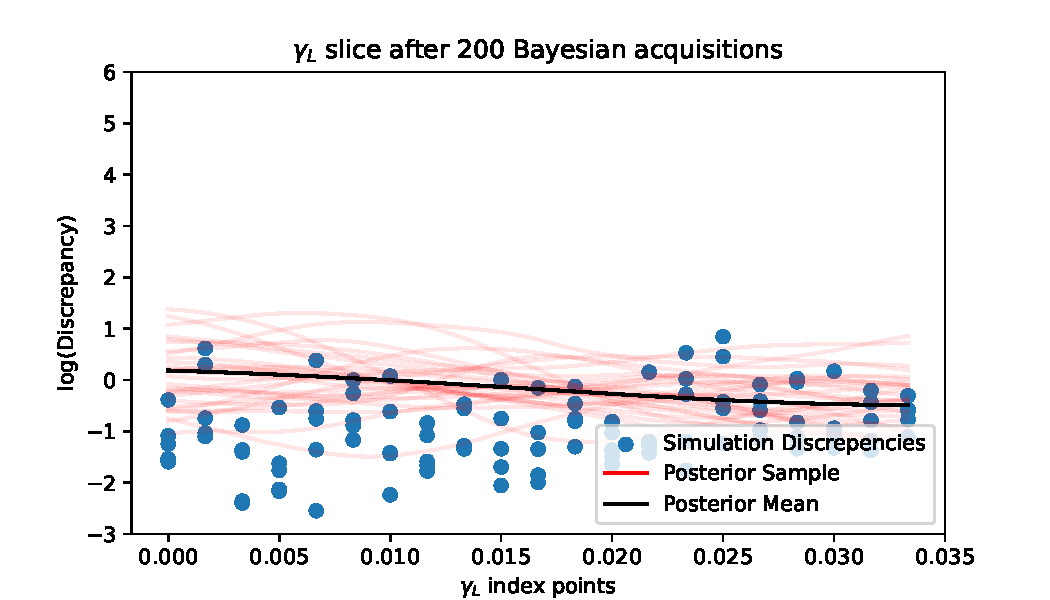
\includegraphics[width=\textwidth]{
            ../champagne_GP_images/gamma_L_slice_200_bolfi_updates_log_discrep.pdf
        }
    \end{subfigure}%
    \hfill%
    \begin{subfigure}[b]{0.5\textwidth}
        \centering
        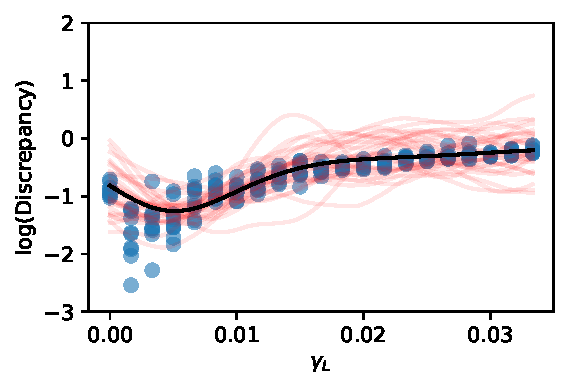
\includegraphics[width=\textwidth]{
            ../champagne_GP_images/gamma_L_slice_300_bolfi_updates_log_discrep.pdf
        }
    \end{subfigure}%
    \hfill%
    \begin{subfigure}[b]{0.5\textwidth}
        \centering
        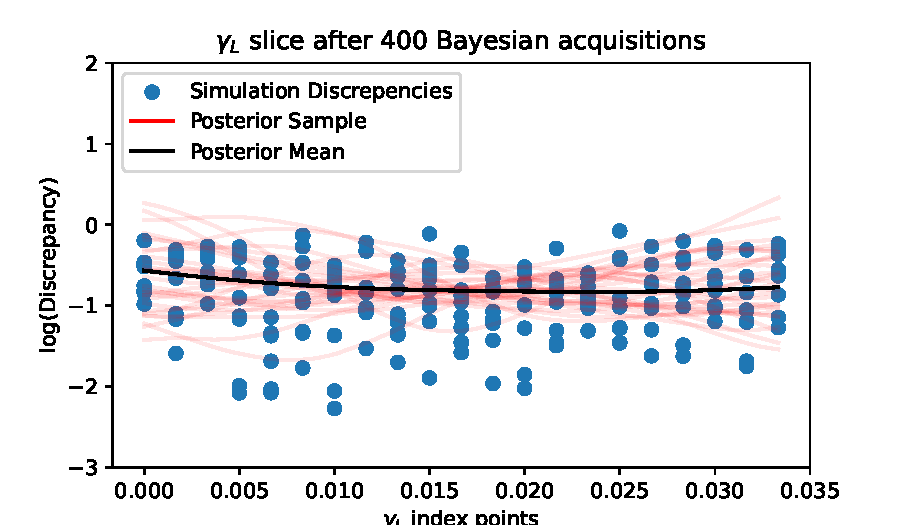
\includegraphics[width=\textwidth]{
            ../champagne_GP_images/gamma_L_slice_400_bolfi_updates_log_discrep.pdf
        }
    \end{subfigure}
    \caption[{
        Gaussian process regression on $\gamma_L$ over time
    }]{
        $d_\GP^{(t)}(\btheta)$ approximation of $\E(\ln\D(\btheta)),$ 
        for $t= 0$, $100$, $200$, $300$, and $400.$ Only $\gamma_L$ was 
        varied. All other parameters were fixed at the true values. Black line 
        is
        $\E(d^{(i)}(\btheta)).$
        Blue dots are realisations from $\ln\D(\btheta).$
    }
\end{figure}

\begin{figure}[htbp]
    \centering
    \begin{subfigure}[b]{0.5\textwidth}
        \centering
        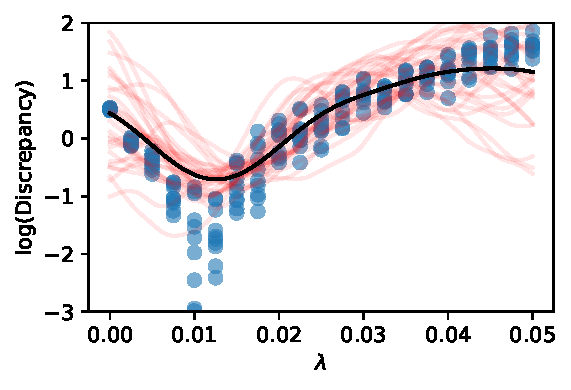
\includegraphics[width=\textwidth]{
            ../champagne_GP_images/initial_lambda_slice_log_discrep.pdf
        }
    \end{subfigure}%
    \hfill%
    \begin{subfigure}[b]{0.5\textwidth}
        \centering
        \includegraphics[width=\textwidth]{
            ../champagne_GP_images/lambda_slice_100_bolfi_updates_log_discrep.pdf
        }
    \end{subfigure}
    \hfill%
    \begin{subfigure}[b]{0.5\textwidth}
        \centering
        \includegraphics[width=\textwidth]{
            ../champagne_GP_images/lambda_slice_200_bolfi_updates_log_discrep.pdf
        }
    \end{subfigure}%
    \hfill%
    \begin{subfigure}[b]{0.5\textwidth}
        \centering
        \includegraphics[width=\textwidth]{
            ../champagne_GP_images/lambda_slice_300_bolfi_updates_log_discrep.pdf
        }
    \end{subfigure}%
    \hfill%
    \begin{subfigure}[b]{0.5\textwidth}
        \centering
        \includegraphics[width=\textwidth]{
            ../champagne_GP_images/lambda_slice_400_bolfi_updates_log_discrep.pdf
        }
    \end{subfigure}
    \caption[{
        Gaussian process regression on $\lambda$ over time
    }]{
        $d_\GP^{(t)}(\btheta)$ approximation of $\E(\ln\D(\btheta)),$ 
        for $t= 0$, $100$, $200$, $300$, and $400.$ Only $\lambda$ was 
        varied. All other parameters were fixed at the true values. Black line 
        is
        $\E(d^{(i)}(\btheta)).$
        Blue dots are realisations from $\ln\D(\btheta).$
    }
\end{figure}

\begin{figure}[htbp]
    \centering
    \begin{subfigure}[b]{0.5\textwidth}
        \centering
        \includegraphics[width=\textwidth]{
            ../champagne_GP_images/initial_f_slice_log_discrep.pdf
        }
    \end{subfigure}%
    \hfill%
    \begin{subfigure}[b]{0.5\textwidth}
        \centering
        \includegraphics[width=\textwidth]{
            ../champagne_GP_images/f_slice_100_bolfi_updates_log_discrep.pdf
        }
    \end{subfigure}
    \hfill%
    \begin{subfigure}[b]{0.5\textwidth}
        \centering
        \includegraphics[width=\textwidth]{
            ../champagne_GP_images/f_slice_200_bolfi_updates_log_discrep.pdf
        }
    \end{subfigure}%
    \hfill%
    \begin{subfigure}[b]{0.5\textwidth}
        \centering
        \includegraphics[width=\textwidth]{
            ../champagne_GP_images/f_slice_300_bolfi_updates_log_discrep.pdf
        }
    \end{subfigure}%
    \hfill%
    \begin{subfigure}[b]{0.5\textwidth}
        \centering
        \includegraphics[width=\textwidth]{
            ../champagne_GP_images/f_slice_400_bolfi_updates_log_discrep.pdf
        }
    \end{subfigure}
    \caption[{
        Gaussian process regression on $f$ over time
    }]{
        $d_\GP^{(t)}(\btheta)$ approximation of $\E(\ln\D(\btheta)),$ 
        for $t= 0$, $100$, $200$, $300$, and $400.$ Only $f$ was 
        varied. All other parameters were fixed at the true values. Black line 
        is
        $\E(d^{(i)}(\btheta)).$
        Blue dots are realisations from $\ln\D(\btheta).$
    }
\end{figure}

\begin{figure}[htbp]
    \centering
    \begin{subfigure}[b]{0.5\textwidth}
        \centering
        \includegraphics[width=\textwidth]{
            ../champagne_GP_images/initial_r_slice_log_discrep.pdf
        }
    \end{subfigure}%
    \hfill%
    \begin{subfigure}[b]{0.5\textwidth}
        \centering
        \includegraphics[width=\textwidth]{
            ../champagne_GP_images/r_slice_100_bolfi_updates_log_discrep.pdf
        }
    \end{subfigure}
    \hfill%
    \begin{subfigure}[b]{0.5\textwidth}
        \centering
        \includegraphics[width=\textwidth]{
            ../champagne_GP_images/r_slice_200_bolfi_updates_log_discrep.pdf
        }
    \end{subfigure}%
    \hfill%
    \begin{subfigure}[b]{0.5\textwidth}
        \centering
        \includegraphics[width=\textwidth]{
            ../champagne_GP_images/r_slice_300_bolfi_updates_log_discrep.pdf
        }
    \end{subfigure}%
    \hfill%
    \begin{subfigure}[b]{0.5\textwidth}
        \centering
        \includegraphics[width=\textwidth]{
            ../champagne_GP_images/r_slice_400_bolfi_updates_log_discrep.pdf
        }
    \end{subfigure}
    \caption[{
        Gaussian process regression on $r$ over time
    }]{
        $d_\GP^{(t)}(\btheta)$ approximation of $\E(\ln\D(\btheta)),$ 
        for $t= 0$, $100$, $200$, $300$, and $400.$ Only $r$ was 
        varied. All other parameters were fixed at the true values. Black line 
        is
        $\E(d^{(i)}(\btheta)).$
        Blue dots are realisations from $\ln\D(\btheta).$
    }
\end{figure}
\end{document}